\documentclass[twoside]{book}

% Packages required by doxygen
\usepackage{fixltx2e}
\usepackage{calc}
\usepackage{doxygen}
\usepackage[export]{adjustbox} % also loads graphicx
\usepackage{graphicx}
\usepackage[utf8]{inputenc}
\usepackage{makeidx}
\usepackage{multicol}
\usepackage{multirow}
\PassOptionsToPackage{warn}{textcomp}
\usepackage{textcomp}
\usepackage[nointegrals]{wasysym}
\usepackage[table]{xcolor}

% Font selection
\usepackage[T1]{fontenc}
\usepackage[scaled=.90]{helvet}
\usepackage{courier}
\usepackage{amssymb}
\usepackage{sectsty}
\renewcommand{\familydefault}{\sfdefault}
\allsectionsfont{%
  \fontseries{bc}\selectfont%
  \color{darkgray}%
}
\renewcommand{\DoxyLabelFont}{%
  \fontseries{bc}\selectfont%
  \color{darkgray}%
}
\newcommand{\+}{\discretionary{\mbox{\scriptsize$\hookleftarrow$}}{}{}}

% Page & text layout
\usepackage{geometry}
\geometry{%
  a4paper,%
  top=2.5cm,%
  bottom=2.5cm,%
  left=2.5cm,%
  right=2.5cm%
}
\tolerance=750
\hfuzz=15pt
\hbadness=750
\setlength{\emergencystretch}{15pt}
\setlength{\parindent}{0cm}
\setlength{\parskip}{0.2cm}
\makeatletter
\renewcommand{\paragraph}{%
  \@startsection{paragraph}{4}{0ex}{-1.0ex}{1.0ex}{%
    \normalfont\normalsize\bfseries\SS@parafont%
  }%
}
\renewcommand{\subparagraph}{%
  \@startsection{subparagraph}{5}{0ex}{-1.0ex}{1.0ex}{%
    \normalfont\normalsize\bfseries\SS@subparafont%
  }%
}
\makeatother

% Headers & footers
\usepackage{fancyhdr}
\pagestyle{fancyplain}
\fancyhead[LE]{\fancyplain{}{\bfseries\thepage}}
\fancyhead[CE]{\fancyplain{}{}}
\fancyhead[RE]{\fancyplain{}{\bfseries\leftmark}}
\fancyhead[LO]{\fancyplain{}{\bfseries\rightmark}}
\fancyhead[CO]{\fancyplain{}{}}
\fancyhead[RO]{\fancyplain{}{\bfseries\thepage}}
\fancyfoot[LE]{\fancyplain{}{}}
\fancyfoot[CE]{\fancyplain{}{}}
\fancyfoot[RE]{\fancyplain{}{\bfseries\scriptsize Generated on Wed May 13 2015 18\+:44\+:21 for Irrigation test system 1 by Doxygen }}
\fancyfoot[LO]{\fancyplain{}{\bfseries\scriptsize Generated on Wed May 13 2015 18\+:44\+:21 for Irrigation test system 1 by Doxygen }}
\fancyfoot[CO]{\fancyplain{}{}}
\fancyfoot[RO]{\fancyplain{}{}}
\renewcommand{\footrulewidth}{0.4pt}
\renewcommand{\chaptermark}[1]{%
  \markboth{#1}{}%
}
\renewcommand{\sectionmark}[1]{%
  \markright{\thesection\ #1}%
}

% Indices & bibliography
\usepackage{natbib}
\usepackage[titles]{tocloft}
\setcounter{tocdepth}{3}
\setcounter{secnumdepth}{5}
\makeindex

% Hyperlinks (required, but should be loaded last)
\usepackage{ifpdf}
\ifpdf
  \usepackage[pdftex,pagebackref=true]{hyperref}
\else
  \usepackage[ps2pdf,pagebackref=true]{hyperref}
\fi
\hypersetup{%
  colorlinks=true,%
  linkcolor=blue,%
  citecolor=blue,%
  unicode%
}

% Custom commands
\newcommand{\clearemptydoublepage}{%
  \newpage{\pagestyle{empty}\cleardoublepage}%
}


%===== C O N T E N T S =====

\begin{document}

% Titlepage & ToC
\hypersetup{pageanchor=false,
             bookmarks=true,
             bookmarksnumbered=true,
             pdfencoding=unicode
            }
\pagenumbering{roman}
\begin{titlepage}
\vspace*{7cm}
\begin{center}%
{\Large Irrigation test system 1 }\\
\vspace*{1cm}
{\large Generated by Doxygen 1.8.9.1}\\
\vspace*{0.5cm}
{\small Wed May 13 2015 18:44:21}\\
\end{center}
\end{titlepage}
\clearemptydoublepage
\tableofcontents
\clearemptydoublepage
\pagenumbering{arabic}
\hypersetup{pageanchor=true}

%--- Begin generated contents ---
\chapter{Todo List}
\label{todo}
\hypertarget{todo}{}

\begin{DoxyRefList}
\item[\label{todo__todo000001}%
\hypertarget{todo__todo000001}{}%
File \hyperlink{hw_8h}{hw.h} ]There is some stuff not belonging to this file in here, it should be moved 
\item[\label{todo__todo000002}%
\hypertarget{todo__todo000002}{}%
global\+Scope$>$ Member \hyperlink{hw_8h_a3c02952100e7d051b77cdf060ca0ba9ba45012c00c17031e71a4f60ada04df07d}{H\+W\+\_\+\+I\+N\+I\+T\+\_\+\+P\+R\+E\+\_\+\+N\+V\+I\+C} ]Implement the default value thing  
\item[\label{todo__todo000004}%
\hypertarget{todo__todo000004}{}%
Member \hyperlink{structirrigation__controller__status_ab795e232c4e2d405b11e24312a6163c3}{irrigation\+\_\+controller\+\_\+status\+:\+:last\+\_\+hot\+\_\+sample} ]Clean up unused stuff here  
\item[\label{todo__todo000005}%
\hypertarget{todo__todo000005}{}%
File \hyperlink{main_8c}{main.c} ]systick, adc, moisture sensor, pwm output, filter 
\item[\label{todo__todo000003}%
\hypertarget{todo__todo000003}{}%
global\+Scope$>$ Member \hyperlink{irrigation_8h_a9891f6b3b37611d2aebdb8601acdf6c6a4460d045ceb966a377b72d2825606fbd}{moisture\+\_\+sensor\+\_\+t1} ]t1 and t2 are not used for the moment 
\end{DoxyRefList}
\chapter{Module Index}
\section{Modules}
Here is a list of all modules\+:\begin{DoxyCompactList}
\item \contentsline{section}{Initial state}{\pageref{group__state__init}}{}
\item \contentsline{section}{Sensor validation state}{\pageref{group__state__validate}}{}
\item \contentsline{section}{Reboot state}{\pageref{group__state__reboot}}{}
\item \contentsline{section}{This state makes the actual soil measure}{\pageref{group__state__measure}}{}
\item \contentsline{section}{The main state machine}{\pageref{group__state__machine}}{}
\item \contentsline{section}{Where the hardware is controlled}{\pageref{group__hardware__control}}{}
\end{DoxyCompactList}

\chapter{Hierarchical Index}
\section{Class Hierarchy}
This inheritance list is sorted roughly, but not completely, alphabetically\+:\begin{DoxyCompactList}
\item \contentsline{section}{adc}{\pageref{structadc}}{}
\item \contentsline{section}{adc\+\_\+config}{\pageref{structadc__config}}{}
\item \contentsline{section}{v3.\+box3}{\pageref{classv3_1_1box3}}{}
\item \contentsline{section}{colour.\+C\+\_\+\+H\+E\+X}{\pageref{classcolour_1_1C__HEX}}{}
\item \contentsline{section}{colour.\+C\+\_\+\+R\+G\+B}{\pageref{classcolour_1_1C__RGB}}{}
\item \contentsline{section}{lampa4.\+cball}{\pageref{classlampa4_1_1cball}}{}
\item \contentsline{section}{lampa\+\_\+searchlight.\+cball}{\pageref{classlampa__searchlight_1_1cball}}{}
\item \contentsline{section}{lampa3.\+cball}{\pageref{classlampa3_1_1cball}}{}
\item \contentsline{section}{color}{\pageref{structcolor}}{}
\item \contentsline{section}{filter\+\_\+rms}{\pageref{structfilter__rms}}{}
\item \contentsline{section}{filter\+\_\+sample\+\_\+range}{\pageref{structfilter__sample__range}}{}
\item \contentsline{section}{gpio\+\_\+pin}{\pageref{structgpio__pin}}{}
\item \contentsline{section}{gpio\+\_\+pin\+\_\+config}{\pageref{structgpio__pin__config}}{}
\item \contentsline{section}{gpio\+\_\+port}{\pageref{structgpio__port}}{}
\item \contentsline{section}{gpio\+\_\+port\+\_\+config}{\pageref{structgpio__port__config}}{}
\item \contentsline{section}{colour.\+H\+S\+L}{\pageref{classcolour_1_1HSL}}{}
\item \contentsline{section}{irrigation\+\_\+controller}{\pageref{structirrigation__controller}}{}
\item \contentsline{section}{irrigation\+\_\+controller\+\_\+status}{\pageref{structirrigation__controller__status}}{}
\item \contentsline{section}{irrigation\+\_\+events}{\pageref{structirrigation__events}}{}
\item \contentsline{section}{irrigation\+\_\+temperature\+\_\+sample}{\pageref{structirrigation__temperature__sample}}{}
\item \contentsline{section}{test\+\_\+lamp\+\_\+2.\+L\+E\+D}{\pageref{classtest__lamp__2_1_1LED}}{}
\item object\begin{DoxyCompactList}
\item \contentsline{section}{colour.\+Color}{\pageref{classcolour_1_1Color}}{}
\end{DoxyCompactList}
\item \contentsline{section}{sample\+\_\+range}{\pageref{structsample__range}}{}
\item \contentsline{section}{state}{\pageref{structstate}}{}
\item \contentsline{section}{sw\+\_\+timer\+\_\+system\+\_\+time}{\pageref{structsw__timer__system__time}}{}
\item \contentsline{section}{systick}{\pageref{structsystick}}{}
\item \contentsline{section}{systick\+\_\+config}{\pageref{structsystick__config}}{}
\item \contentsline{section}{timer}{\pageref{structtimer}}{}
\item \contentsline{section}{timer\+\_\+ccr}{\pageref{structtimer__ccr}}{}
\item \contentsline{section}{timer\+\_\+ccr\+\_\+config}{\pageref{structtimer__ccr__config}}{}
\item \contentsline{section}{timer\+\_\+config}{\pageref{structtimer__config}}{}
\item \contentsline{section}{tm}{\pageref{structtm}}{}
\item \contentsline{section}{usart}{\pageref{structusart}}{}
\item \contentsline{section}{usart\+\_\+config}{\pageref{structusart__config}}{}
\item \contentsline{section}{v3.\+vec3}{\pageref{classv3_1_1vec3}}{}
\item \contentsline{section}{ws2812}{\pageref{structws2812}}{}
\item \contentsline{section}{ws2812\+\_\+config}{\pageref{structws2812__config}}{}
\item \contentsline{section}{ws2812\+\_\+rgb}{\pageref{structws2812__rgb}}{}
\end{DoxyCompactList}

\chapter{Class Index}
\section{Class List}
Here are the classes, structs, unions and interfaces with brief descriptions\+:\begin{DoxyCompactList}
\item\contentsline{section}{\hyperlink{structadc}{adc} }{\pageref{structadc}}{}
\item\contentsline{section}{\hyperlink{structadc__config}{adc\+\_\+config} }{\pageref{structadc__config}}{}
\item\contentsline{section}{\hyperlink{classv3_1_1box3}{v3.\+box3} }{\pageref{classv3_1_1box3}}{}
\item\contentsline{section}{\hyperlink{classcolour_1_1C__HEX}{colour.\+C\+\_\+\+H\+E\+X} }{\pageref{classcolour_1_1C__HEX}}{}
\item\contentsline{section}{\hyperlink{classcolour_1_1C__RGB}{colour.\+C\+\_\+\+R\+G\+B} }{\pageref{classcolour_1_1C__RGB}}{}
\item\contentsline{section}{\hyperlink{classlampa4_1_1cball}{lampa4.\+cball} }{\pageref{classlampa4_1_1cball}}{}
\item\contentsline{section}{\hyperlink{classlampa__searchlight_1_1cball}{lampa\+\_\+searchlight.\+cball} }{\pageref{classlampa__searchlight_1_1cball}}{}
\item\contentsline{section}{\hyperlink{classlampa3_1_1cball}{lampa3.\+cball} }{\pageref{classlampa3_1_1cball}}{}
\item\contentsline{section}{\hyperlink{classcolour_1_1Color}{colour.\+Color} \\*All purpose object }{\pageref{classcolour_1_1Color}}{}
\item\contentsline{section}{\hyperlink{structcolor}{color} }{\pageref{structcolor}}{}
\item\contentsline{section}{\hyperlink{structfilter__rms}{filter\+\_\+rms} }{\pageref{structfilter__rms}}{}
\item\contentsline{section}{\hyperlink{structfilter__sample__range}{filter\+\_\+sample\+\_\+range} }{\pageref{structfilter__sample__range}}{}
\item\contentsline{section}{\hyperlink{structgpio__pin}{gpio\+\_\+pin} }{\pageref{structgpio__pin}}{}
\item\contentsline{section}{\hyperlink{structgpio__pin__config}{gpio\+\_\+pin\+\_\+config} }{\pageref{structgpio__pin__config}}{}
\item\contentsline{section}{\hyperlink{structgpio__port}{gpio\+\_\+port} }{\pageref{structgpio__port}}{}
\item\contentsline{section}{\hyperlink{structgpio__port__config}{gpio\+\_\+port\+\_\+config} }{\pageref{structgpio__port__config}}{}
\item\contentsline{section}{\hyperlink{classcolour_1_1HSL}{colour.\+H\+S\+L} }{\pageref{classcolour_1_1HSL}}{}
\item\contentsline{section}{\hyperlink{structirrigation__controller}{irrigation\+\_\+controller} \\*Holds everything related to the irrigation controller }{\pageref{structirrigation__controller}}{}
\item\contentsline{section}{\hyperlink{structirrigation__controller__status}{irrigation\+\_\+controller\+\_\+status} }{\pageref{structirrigation__controller__status}}{}
\item\contentsline{section}{\hyperlink{structirrigation__events}{irrigation\+\_\+events} \\*The event callback functions for the irrigation controller core }{\pageref{structirrigation__events}}{}
\item\contentsline{section}{\hyperlink{structirrigation__temperature__sample}{irrigation\+\_\+temperature\+\_\+sample} \\*This is a timestamped temperature sample }{\pageref{structirrigation__temperature__sample}}{}
\item\contentsline{section}{\hyperlink{classtest__lamp__2_1_1LED}{test\+\_\+lamp\+\_\+2.\+L\+E\+D} }{\pageref{classtest__lamp__2_1_1LED}}{}
\item\contentsline{section}{\hyperlink{structsample__range}{sample\+\_\+range} }{\pageref{structsample__range}}{}
\item\contentsline{section}{\hyperlink{structstate}{state} }{\pageref{structstate}}{}
\item\contentsline{section}{\hyperlink{structsw__timer__system__time}{sw\+\_\+timer\+\_\+system\+\_\+time} }{\pageref{structsw__timer__system__time}}{}
\item\contentsline{section}{\hyperlink{structsystick}{systick} }{\pageref{structsystick}}{}
\item\contentsline{section}{\hyperlink{structsystick__config}{systick\+\_\+config} }{\pageref{structsystick__config}}{}
\item\contentsline{section}{\hyperlink{structtimer}{timer} }{\pageref{structtimer}}{}
\item\contentsline{section}{\hyperlink{structtimer__ccr}{timer\+\_\+ccr} }{\pageref{structtimer__ccr}}{}
\item\contentsline{section}{\hyperlink{structtimer__ccr__config}{timer\+\_\+ccr\+\_\+config} }{\pageref{structtimer__ccr__config}}{}
\item\contentsline{section}{\hyperlink{structtimer__config}{timer\+\_\+config} }{\pageref{structtimer__config}}{}
\item\contentsline{section}{\hyperlink{structtm}{tm} }{\pageref{structtm}}{}
\item\contentsline{section}{\hyperlink{structusart}{usart} }{\pageref{structusart}}{}
\item\contentsline{section}{\hyperlink{structusart__config}{usart\+\_\+config} }{\pageref{structusart__config}}{}
\item\contentsline{section}{\hyperlink{classv3_1_1vec3}{v3.\+vec3} }{\pageref{classv3_1_1vec3}}{}
\item\contentsline{section}{\hyperlink{structws2812}{ws2812} }{\pageref{structws2812}}{}
\item\contentsline{section}{\hyperlink{structws2812__config}{ws2812\+\_\+config} }{\pageref{structws2812__config}}{}
\item\contentsline{section}{\hyperlink{structws2812__rgb}{ws2812\+\_\+rgb} }{\pageref{structws2812__rgb}}{}
\end{DoxyCompactList}

\chapter{File Index}
\section{File List}
Here is a list of all documented files with brief descriptions\+:\begin{DoxyCompactList}
\item\contentsline{section}{src/{\bfseries adc.\+h} }{\pageref{adc_8h}}{}
\item\contentsline{section}{src/{\bfseries color.\+h} }{\pageref{color_8h}}{}
\item\contentsline{section}{src/{\bfseries common.\+h} }{\pageref{common_8h}}{}
\item\contentsline{section}{src/{\bfseries dma.\+h} }{\pageref{dma_8h}}{}
\item\contentsline{section}{src/{\bfseries filter.\+h} }{\pageref{filter_8h}}{}
\item\contentsline{section}{src/{\bfseries gpio.\+h} }{\pageref{gpio_8h}}{}
\item\contentsline{section}{src/{\bfseries gpio\+\_\+macro.\+h} }{\pageref{gpio__macro_8h}}{}
\item\contentsline{section}{src/\hyperlink{hw_8h}{hw.\+h} \\*Hardware abstraction layer include file }{\pageref{hw_8h}}{}
\item\contentsline{section}{src/\hyperlink{irrigation_8h}{irrigation.\+h} \\*Irrigation main include file }{\pageref{irrigation_8h}}{}
\item\contentsline{section}{src/{\bfseries led.\+h} }{\pageref{led_8h}}{}
\item\contentsline{section}{src/{\bfseries led\+\_\+macro.\+h} }{\pageref{led__macro_8h}}{}
\item\contentsline{section}{src/\hyperlink{main_8c}{main.\+c} \\*Irrigation controller main file }{\pageref{main_8c}}{}
\item\contentsline{section}{src/{\bfseries math.\+h} }{\pageref{math_8h}}{}
\item\contentsline{section}{src/{\bfseries moisture\+\_\+sensor.\+h} }{\pageref{moisture__sensor_8h}}{}
\item\contentsline{section}{src/{\bfseries msg.\+h} }{\pageref{msg_8h}}{}
\item\contentsline{section}{src/{\bfseries pump.\+h} }{\pageref{pump_8h}}{}
\item\contentsline{section}{src/\hyperlink{state__init_8c}{state\+\_\+init.\+c} \\*Initial state }{\pageref{state__init_8c}}{}
\item\contentsline{section}{src/\hyperlink{state__measure_8c}{state\+\_\+measure.\+c} \\*Measurement state }{\pageref{state__measure_8c}}{}
\item\contentsline{section}{src/\hyperlink{state__reboot_8c}{state\+\_\+reboot.\+c} \\*Rebooting state }{\pageref{state__reboot_8c}}{}
\item\contentsline{section}{src/\hyperlink{state__validate_8c}{state\+\_\+validate.\+c} \\*Sensor validation state }{\pageref{state__validate_8c}}{}
\item\contentsline{section}{src/{\bfseries systick.\+h} }{\pageref{systick_8h}}{}
\item\contentsline{section}{src/{\bfseries time.\+h} }{\pageref{time_8h}}{}
\item\contentsline{section}{src/{\bfseries timer.\+h} }{\pageref{timer_8h}}{}
\item\contentsline{section}{src/{\bfseries timer\+\_\+macro.\+h} }{\pageref{timer__macro_8h}}{}
\item\contentsline{section}{src/{\bfseries uart.\+h} }{\pageref{uart_8h}}{}
\item\contentsline{section}{src/{\bfseries usart\+\_\+macro.\+h} }{\pageref{usart__macro_8h}}{}
\item\contentsline{section}{src/{\bfseries ws2812.\+h} }{\pageref{ws2812_8h}}{}
\item\contentsline{section}{src/{\bfseries ws2812\+\_\+macro.\+h} }{\pageref{ws2812__macro_8h}}{}
\end{DoxyCompactList}

\chapter{Module Documentation}
\hypertarget{group__state__init}{}\section{Initial state}
\label{group__state__init}\index{Initial state@{Initial state}}
\subsection*{Functions}
\begin{DoxyCompactItemize}
\item 
void \hyperlink{group__state__init_gaeca2f683660bf42f5258acd6aac353d0}{state\+\_\+init\+\_\+enter} (struct \hyperlink{structirrigation__controller}{irrigation\+\_\+controller} $\ast$controller)
\begin{DoxyCompactList}\small\item\em Reset all variables in the controller this state uses. \end{DoxyCompactList}\item 
void \hyperlink{group__state__init_ga5b5f5a7ec8534a643fb599efdee6ed4f}{state\+\_\+init\+\_\+run} (struct \hyperlink{structirrigation__controller}{irrigation\+\_\+controller} $\ast$controller)
\begin{DoxyCompactList}\small\item\em We will make a heart beat ramp for the status L\+E\+D while we wait for initial delay to complete. \end{DoxyCompactList}\item 
void \hyperlink{group__state__init_ga52863e306edb45d15c12acdecb7e5555}{state\+\_\+init\+\_\+exit} (struct \hyperlink{structirrigation__controller}{irrigation\+\_\+controller} $\ast$controller)
\begin{DoxyCompactList}\small\item\em Nothing has do be done before we leave this state. \end{DoxyCompactList}\end{DoxyCompactItemize}


\subsection{Detailed Description}


\subsection{Function Documentation}
\hypertarget{group__state__init_gaeca2f683660bf42f5258acd6aac353d0}{}\index{Initial state@{Initial state}!state\+\_\+init\+\_\+enter@{state\+\_\+init\+\_\+enter}}
\index{state\+\_\+init\+\_\+enter@{state\+\_\+init\+\_\+enter}!Initial state@{Initial state}}
\subsubsection[{state\+\_\+init\+\_\+enter}]{\setlength{\rightskip}{0pt plus 5cm}void state\+\_\+init\+\_\+enter (
\begin{DoxyParamCaption}
\item[{struct {\bf irrigation\+\_\+controller} $\ast$}]{controller}
\end{DoxyParamCaption}
)}\label{group__state__init_gaeca2f683660bf42f5258acd6aac353d0}


Reset all variables in the controller this state uses. 

\hypertarget{group__state__init_ga52863e306edb45d15c12acdecb7e5555}{}\index{Initial state@{Initial state}!state\+\_\+init\+\_\+exit@{state\+\_\+init\+\_\+exit}}
\index{state\+\_\+init\+\_\+exit@{state\+\_\+init\+\_\+exit}!Initial state@{Initial state}}
\subsubsection[{state\+\_\+init\+\_\+exit}]{\setlength{\rightskip}{0pt plus 5cm}void state\+\_\+init\+\_\+exit (
\begin{DoxyParamCaption}
\item[{struct {\bf irrigation\+\_\+controller} $\ast$}]{controller}
\end{DoxyParamCaption}
)}\label{group__state__init_ga52863e306edb45d15c12acdecb7e5555}


Nothing has do be done before we leave this state. 

\hypertarget{group__state__init_ga5b5f5a7ec8534a643fb599efdee6ed4f}{}\index{Initial state@{Initial state}!state\+\_\+init\+\_\+run@{state\+\_\+init\+\_\+run}}
\index{state\+\_\+init\+\_\+run@{state\+\_\+init\+\_\+run}!Initial state@{Initial state}}
\subsubsection[{state\+\_\+init\+\_\+run}]{\setlength{\rightskip}{0pt plus 5cm}void state\+\_\+init\+\_\+run (
\begin{DoxyParamCaption}
\item[{struct {\bf irrigation\+\_\+controller} $\ast$}]{controller}
\end{DoxyParamCaption}
)}\label{group__state__init_ga5b5f5a7ec8534a643fb599efdee6ed4f}


We will make a heart beat ramp for the status L\+E\+D while we wait for initial delay to complete. 


\hypertarget{group__state__validate}{}\section{Sensor validation state}
\label{group__state__validate}\index{Sensor validation state@{Sensor validation state}}
\subsection*{Functions}
\begin{DoxyCompactItemize}
\item 
void \hyperlink{group__state__validate_gac0d41d4685bd461b3a613f6320405b79}{state\+\_\+validate\+\_\+enter} (struct \hyperlink{structirrigation__controller}{irrigation\+\_\+controller} $\ast$controller)
\begin{DoxyCompactList}\small\item\em We set up the validation timer and init the maximum and minim temperatured. \end{DoxyCompactList}\item 
void \hyperlink{group__state__validate_gaec38509b93f8a850919aa7a36e543ed5}{state\+\_\+validate\+\_\+run} (struct \hyperlink{structirrigation__controller}{irrigation\+\_\+controller} $\ast$controller)
\begin{DoxyCompactList}\small\item\em We have the heart beat L\+E\+D status and we update the minimum and maximum values while we continue to sample sensor data. \end{DoxyCompactList}\item 
void \hyperlink{group__state__validate_gac480e756742ffd9acd9bd21ac1e8885c}{state\+\_\+validate\+\_\+exit} (struct \hyperlink{structirrigation__controller}{irrigation\+\_\+controller} $\ast$controller)
\begin{DoxyCompactList}\small\item\em Nothing has to be done when we exit this state. \end{DoxyCompactList}\end{DoxyCompactItemize}


\subsection{Detailed Description}


\subsection{Function Documentation}
\hypertarget{group__state__validate_gac0d41d4685bd461b3a613f6320405b79}{}\index{Sensor validation state@{Sensor validation state}!state\+\_\+validate\+\_\+enter@{state\+\_\+validate\+\_\+enter}}
\index{state\+\_\+validate\+\_\+enter@{state\+\_\+validate\+\_\+enter}!Sensor validation state@{Sensor validation state}}
\subsubsection[{state\+\_\+validate\+\_\+enter}]{\setlength{\rightskip}{0pt plus 5cm}void state\+\_\+validate\+\_\+enter (
\begin{DoxyParamCaption}
\item[{struct {\bf irrigation\+\_\+controller} $\ast$}]{controller}
\end{DoxyParamCaption}
)}\label{group__state__validate_gac0d41d4685bd461b3a613f6320405b79}


We set up the validation timer and init the maximum and minim temperatured. 

We also check that we have current sensor data availble \hypertarget{group__state__validate_gac480e756742ffd9acd9bd21ac1e8885c}{}\index{Sensor validation state@{Sensor validation state}!state\+\_\+validate\+\_\+exit@{state\+\_\+validate\+\_\+exit}}
\index{state\+\_\+validate\+\_\+exit@{state\+\_\+validate\+\_\+exit}!Sensor validation state@{Sensor validation state}}
\subsubsection[{state\+\_\+validate\+\_\+exit}]{\setlength{\rightskip}{0pt plus 5cm}void state\+\_\+validate\+\_\+exit (
\begin{DoxyParamCaption}
\item[{struct {\bf irrigation\+\_\+controller} $\ast$}]{controller}
\end{DoxyParamCaption}
)}\label{group__state__validate_gac480e756742ffd9acd9bd21ac1e8885c}


Nothing has to be done when we exit this state. 

\hypertarget{group__state__validate_gaec38509b93f8a850919aa7a36e543ed5}{}\index{Sensor validation state@{Sensor validation state}!state\+\_\+validate\+\_\+run@{state\+\_\+validate\+\_\+run}}
\index{state\+\_\+validate\+\_\+run@{state\+\_\+validate\+\_\+run}!Sensor validation state@{Sensor validation state}}
\subsubsection[{state\+\_\+validate\+\_\+run}]{\setlength{\rightskip}{0pt plus 5cm}void state\+\_\+validate\+\_\+run (
\begin{DoxyParamCaption}
\item[{struct {\bf irrigation\+\_\+controller} $\ast$}]{controller}
\end{DoxyParamCaption}
)}\label{group__state__validate_gaec38509b93f8a850919aa7a36e543ed5}


We have the heart beat L\+E\+D status and we update the minimum and maximum values while we continue to sample sensor data. 

When timeout is reached we verify that the sensor data span is reasonable 
\hypertarget{group__state__reboot}{}\section{Reboot state}
\label{group__state__reboot}\index{Reboot state@{Reboot state}}


This state makes sure the systems exits in a nice way before it starts up again.  


\subsection*{Functions}
\begin{DoxyCompactItemize}
\item 
\hypertarget{group__state__reboot_gab0e3409fa69ff96792cb5a768928a545}{}void {\bfseries state\+\_\+reboot\+\_\+enter} (struct \hyperlink{structirrigation__controller}{irrigation\+\_\+controller} $\ast$controller)\label{group__state__reboot_gab0e3409fa69ff96792cb5a768928a545}

\item 
\hypertarget{group__state__reboot_ga23cf1ecfb670c7c6c253a40705aa5caf}{}void {\bfseries state\+\_\+reboot\+\_\+run} (struct \hyperlink{structirrigation__controller}{irrigation\+\_\+controller} $\ast$controller)\label{group__state__reboot_ga23cf1ecfb670c7c6c253a40705aa5caf}

\item 
\hypertarget{group__state__reboot_gafbcdeb4b017f4350fb6ff51df410228b}{}void {\bfseries state\+\_\+reboot\+\_\+exit} (struct \hyperlink{structirrigation__controller}{irrigation\+\_\+controller} $\ast$controller)\label{group__state__reboot_gafbcdeb4b017f4350fb6ff51df410228b}

\end{DoxyCompactItemize}


\subsection{Detailed Description}
This state makes sure the systems exits in a nice way before it starts up again. 


\hypertarget{group__state__measure}{}\section{This state makes the actual soil measure}
\label{group__state__measure}\index{This state makes the actual soil measure@{This state makes the actual soil measure}}
\subsection*{Functions}
\begin{DoxyCompactItemize}
\item 
\hypertarget{group__state__measure_ga24a42892ba25be220bff68fc151e0be7}{}void {\bfseries state\+\_\+measure\+\_\+enter} (struct \hyperlink{structirrigation__controller}{irrigation\+\_\+controller} $\ast$controller)\label{group__state__measure_ga24a42892ba25be220bff68fc151e0be7}

\item 
\hypertarget{group__state__measure_ga410776694bde81bde92a0b6b178ac015}{}void {\bfseries state\+\_\+measure\+\_\+run} (struct \hyperlink{structirrigation__controller}{irrigation\+\_\+controller} $\ast$controller)\label{group__state__measure_ga410776694bde81bde92a0b6b178ac015}

\item 
\hypertarget{group__state__measure_ga0f85f8645f5311e776e85a3697517266}{}void {\bfseries state\+\_\+measure\+\_\+exit} (struct \hyperlink{structirrigation__controller}{irrigation\+\_\+controller} $\ast$controller)\label{group__state__measure_ga0f85f8645f5311e776e85a3697517266}

\end{DoxyCompactItemize}


\subsection{Detailed Description}

\hypertarget{group__state__machine}{}\section{The main state machine}
\label{group__state__machine}\index{The main state machine@{The main state machine}}

\hypertarget{group__hardware__control}{}\section{Where the hardware is controlled}
\label{group__hardware__control}\index{Where the hardware is controlled@{Where the hardware is controlled}}
\}@
\chapter{Class Documentation}
\hypertarget{structadc}{}\section{adc Struct Reference}
\label{structadc}\index{adc@{adc}}


Collaboration diagram for adc\+:\nopagebreak
\begin{figure}[H]
\begin{center}
\leavevmode
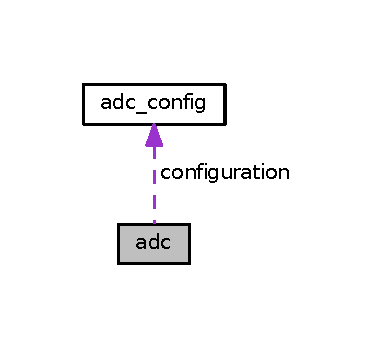
\includegraphics[width=180pt]{structadc__coll__graph}
\end{center}
\end{figure}
\subsection*{Public Attributes}
\begin{DoxyCompactItemize}
\item 
\hypertarget{structadc_aaecb8053d6389a045fd2fd05b3b2f584}{}struct \hyperlink{structadc__config}{adc\+\_\+config} $\ast$ {\bfseries configuration}\label{structadc_aaecb8053d6389a045fd2fd05b3b2f584}

\item 
\hypertarget{structadc_a18f6e4c34b612060add403c39b12c44a}{}uint16\+\_\+t $\ast$ {\bfseries adc\+\_\+buffer}\label{structadc_a18f6e4c34b612060add403c39b12c44a}

\item 
\hypertarget{structadc_a83e9b544b8780ab70e5c193a4b5d8ef8}{}bool {\bfseries sampling\+\_\+done}\label{structadc_a83e9b544b8780ab70e5c193a4b5d8ef8}

\end{DoxyCompactItemize}


The documentation for this struct was generated from the following file\+:\begin{DoxyCompactItemize}
\item 
src/adc.\+h\end{DoxyCompactItemize}

\hypertarget{structadc__config}{}\section{adc\+\_\+config Struct Reference}
\label{structadc__config}\index{adc\+\_\+config@{adc\+\_\+config}}
\subsection*{Public Attributes}
\begin{DoxyCompactItemize}
\item 
\hypertarget{structadc__config_a7f7cc3ba237533dd943faddca7555430}{}uint8\+\_\+t $\ast$ {\bfseries channel\+\_\+map}\label{structadc__config_a7f7cc3ba237533dd943faddca7555430}

\item 
\hypertarget{structadc__config_a33bd54712a72f2dcbd6c3d6d53b776ea}{}int {\bfseries channel\+\_\+count}\label{structadc__config_a33bd54712a72f2dcbd6c3d6d53b776ea}

\end{DoxyCompactItemize}


The documentation for this struct was generated from the following file\+:\begin{DoxyCompactItemize}
\item 
src/adc.\+h\end{DoxyCompactItemize}

\hypertarget{classv3_1_1box3}{}\section{v3.\+box3 Class Reference}
\label{classv3_1_1box3}\index{v3.\+box3@{v3.\+box3}}
\subsection*{Public Member Functions}
\begin{DoxyCompactItemize}
\item 
\hypertarget{classv3_1_1box3_ae0e11ebcc68853135cec1a43454f9ef1}{}def {\bfseries \+\_\+\+\_\+init\+\_\+\+\_\+}\label{classv3_1_1box3_ae0e11ebcc68853135cec1a43454f9ef1}

\item 
\hypertarget{classv3_1_1box3_a42acf62d0f06b489743510649aa63ced}{}def {\bfseries update} (self, pos)\label{classv3_1_1box3_a42acf62d0f06b489743510649aa63ced}

\item 
\hypertarget{classv3_1_1box3_ac6a0cad2aa288c495e5b4339042feb94}{}def {\bfseries bounce} (self, pos, dr)\label{classv3_1_1box3_ac6a0cad2aa288c495e5b4339042feb94}

\item 
\hypertarget{classv3_1_1box3_a62969f1b236a1c75d54f85167b638bc8}{}def {\bfseries grow} (self, amount)\label{classv3_1_1box3_a62969f1b236a1c75d54f85167b638bc8}

\end{DoxyCompactItemize}
\subsection*{Public Attributes}
\begin{DoxyCompactItemize}
\item 
\hypertarget{classv3_1_1box3_a3da80dabc2342f95060a71a67cae5b3c}{}{\bfseries low}\label{classv3_1_1box3_a3da80dabc2342f95060a71a67cae5b3c}

\item 
\hypertarget{classv3_1_1box3_abad1e1f596392a30606ad8d56e9bd4ee}{}{\bfseries high}\label{classv3_1_1box3_abad1e1f596392a30606ad8d56e9bd4ee}

\end{DoxyCompactItemize}


The documentation for this class was generated from the following file\+:\begin{DoxyCompactItemize}
\item 
python\+\_\+scripts/v3.\+py\end{DoxyCompactItemize}

\hypertarget{classcolour_1_1C__HEX}{}\section{colour.\+C\+\_\+\+H\+E\+X Class Reference}
\label{classcolour_1_1C__HEX}\index{colour.\+C\+\_\+\+H\+E\+X@{colour.\+C\+\_\+\+H\+E\+X}}
\subsection*{Public Member Functions}
\begin{DoxyCompactItemize}
\item 
\hypertarget{classcolour_1_1C__HEX_adb239df1b02b06e34849cbd4b30af9f1}{}def {\bfseries \+\_\+\+\_\+getattr\+\_\+\+\_\+} (self, value)\label{classcolour_1_1C__HEX_adb239df1b02b06e34849cbd4b30af9f1}

\end{DoxyCompactItemize}


\subsection{Detailed Description}
\begin{DoxyVerb}RGB colors container

Provides a quick color access.

>>> from colour import HEX

>>> HEX.WHITE
'#fff'
>>> HEX.BLUE
'#00f'

>>> HEX.DONOTEXISTS  # doctest: +ELLIPSIS
Traceback (most recent call last):
...
AttributeError: ... has no attribute 'DONOTEXISTS'\end{DoxyVerb}
 

The documentation for this class was generated from the following file\+:\begin{DoxyCompactItemize}
\item 
python\+\_\+scripts/colour.\+py\end{DoxyCompactItemize}

\hypertarget{classcolour_1_1C__RGB}{}\section{colour.\+C\+\_\+\+R\+G\+B Class Reference}
\label{classcolour_1_1C__RGB}\index{colour.\+C\+\_\+\+R\+G\+B@{colour.\+C\+\_\+\+R\+G\+B}}
\subsection*{Public Member Functions}
\begin{DoxyCompactItemize}
\item 
\hypertarget{classcolour_1_1C__RGB_a043e1602da9fe5ee431a063f0011b3a8}{}def {\bfseries \+\_\+\+\_\+getattr\+\_\+\+\_\+} (self, value)\label{classcolour_1_1C__RGB_a043e1602da9fe5ee431a063f0011b3a8}

\end{DoxyCompactItemize}


\subsection{Detailed Description}
\begin{DoxyVerb}RGB colors container

Provides a quick color access.

>>> from colour import RGB

>>> RGB.WHITE
(1.0, 1.0, 1.0)
>>> RGB.BLUE
(0.0, 0.0, 1.0)

>>> RGB.DONOTEXISTS  # doctest: +ELLIPSIS
Traceback (most recent call last):
...
AttributeError: ... has no attribute 'DONOTEXISTS'\end{DoxyVerb}
 

The documentation for this class was generated from the following file\+:\begin{DoxyCompactItemize}
\item 
python\+\_\+scripts/colour.\+py\end{DoxyCompactItemize}

\hypertarget{classlampa4_1_1cball}{}\section{lampa4.\+cball Class Reference}
\label{classlampa4_1_1cball}\index{lampa4.\+cball@{lampa4.\+cball}}
\subsection*{Public Member Functions}
\begin{DoxyCompactItemize}
\item 
\hypertarget{classlampa4_1_1cball_a95e7de64434c4aba7d6a17060d3a276c}{}def {\bfseries \+\_\+\+\_\+init\+\_\+\+\_\+}\label{classlampa4_1_1cball_a95e7de64434c4aba7d6a17060d3a276c}

\end{DoxyCompactItemize}
\subsection*{Public Attributes}
\begin{DoxyCompactItemize}
\item 
\hypertarget{classlampa4_1_1cball_af268dd90a6c7d1d8175d9ce391af9303}{}{\bfseries pos}\label{classlampa4_1_1cball_af268dd90a6c7d1d8175d9ce391af9303}

\item 
\hypertarget{classlampa4_1_1cball_ab65c346ab6d4871e7776f26ee7ce072a}{}{\bfseries dir}\label{classlampa4_1_1cball_ab65c346ab6d4871e7776f26ee7ce072a}

\item 
\hypertarget{classlampa4_1_1cball_a0cdb91e2a6093e469aad7fb6876c3806}{}{\bfseries color}\label{classlampa4_1_1cball_a0cdb91e2a6093e469aad7fb6876c3806}

\item 
\hypertarget{classlampa4_1_1cball_a7bbf2f00f17d07a52b090055433c720a}{}{\bfseries radius}\label{classlampa4_1_1cball_a7bbf2f00f17d07a52b090055433c720a}

\end{DoxyCompactItemize}


The documentation for this class was generated from the following file\+:\begin{DoxyCompactItemize}
\item 
python\+\_\+scripts/lampa4.\+py\end{DoxyCompactItemize}

\hypertarget{classlampa__searchlight_1_1cball}{}\section{lampa\+\_\+searchlight.\+cball Class Reference}
\label{classlampa__searchlight_1_1cball}\index{lampa\+\_\+searchlight.\+cball@{lampa\+\_\+searchlight.\+cball}}
\subsection*{Public Member Functions}
\begin{DoxyCompactItemize}
\item 
\hypertarget{classlampa__searchlight_1_1cball_a2528956a998c545b51eb13731afea862}{}def {\bfseries \+\_\+\+\_\+init\+\_\+\+\_\+} (self, \hyperlink{structcolor}{color})\label{classlampa__searchlight_1_1cball_a2528956a998c545b51eb13731afea862}

\end{DoxyCompactItemize}
\subsection*{Public Attributes}
\begin{DoxyCompactItemize}
\item 
\hypertarget{classlampa__searchlight_1_1cball_a3e8093b62dddbe8870a529212b883998}{}{\bfseries pos}\label{classlampa__searchlight_1_1cball_a3e8093b62dddbe8870a529212b883998}

\item 
\hypertarget{classlampa__searchlight_1_1cball_af75f99867f287e260a098a8dc531b326}{}{\bfseries dir}\label{classlampa__searchlight_1_1cball_af75f99867f287e260a098a8dc531b326}

\item 
\hypertarget{classlampa__searchlight_1_1cball_af462f24599212a23ea24755056411c9d}{}{\bfseries color}\label{classlampa__searchlight_1_1cball_af462f24599212a23ea24755056411c9d}

\item 
\hypertarget{classlampa__searchlight_1_1cball_ac788a56d2a2abdc72149844f00b2fa8a}{}{\bfseries radius}\label{classlampa__searchlight_1_1cball_ac788a56d2a2abdc72149844f00b2fa8a}

\end{DoxyCompactItemize}


The documentation for this class was generated from the following file\+:\begin{DoxyCompactItemize}
\item 
python\+\_\+scripts/lampa\+\_\+searchlight.\+py\end{DoxyCompactItemize}

\hypertarget{classlampa3_1_1cball}{}\section{lampa3.\+cball Class Reference}
\label{classlampa3_1_1cball}\index{lampa3.\+cball@{lampa3.\+cball}}
\subsection*{Public Member Functions}
\begin{DoxyCompactItemize}
\item 
\hypertarget{classlampa3_1_1cball_a07991d683ccb1f1f86f1117b7507f6c3}{}def {\bfseries \+\_\+\+\_\+init\+\_\+\+\_\+} (self, \hyperlink{structcolor}{color})\label{classlampa3_1_1cball_a07991d683ccb1f1f86f1117b7507f6c3}

\end{DoxyCompactItemize}
\subsection*{Public Attributes}
\begin{DoxyCompactItemize}
\item 
\hypertarget{classlampa3_1_1cball_a9107f79e11da1bdfd757221b1f5de6bc}{}{\bfseries pos}\label{classlampa3_1_1cball_a9107f79e11da1bdfd757221b1f5de6bc}

\item 
\hypertarget{classlampa3_1_1cball_a8bd7b85a3efa502302651ba6f2e6ba52}{}{\bfseries dir}\label{classlampa3_1_1cball_a8bd7b85a3efa502302651ba6f2e6ba52}

\item 
\hypertarget{classlampa3_1_1cball_a1c63ffd2499a64b785636149398010fb}{}{\bfseries color}\label{classlampa3_1_1cball_a1c63ffd2499a64b785636149398010fb}

\item 
\hypertarget{classlampa3_1_1cball_a6af41e5c82a7caccd638fc14e3caf3f9}{}{\bfseries radius}\label{classlampa3_1_1cball_a6af41e5c82a7caccd638fc14e3caf3f9}

\end{DoxyCompactItemize}


The documentation for this class was generated from the following file\+:\begin{DoxyCompactItemize}
\item 
python\+\_\+scripts/lampa3.\+py\end{DoxyCompactItemize}

\hypertarget{classcolour_1_1Color}{}\section{colour.\+Color Class Reference}
\label{classcolour_1_1Color}\index{colour.\+Color@{colour.\+Color}}


All purpose object.  




Inheritance diagram for colour.\+Color\+:\nopagebreak
\begin{figure}[H]
\begin{center}
\leavevmode
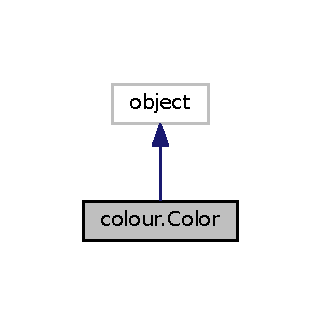
\includegraphics[width=154pt]{classcolour_1_1Color__inherit__graph}
\end{center}
\end{figure}


Collaboration diagram for colour.\+Color\+:\nopagebreak
\begin{figure}[H]
\begin{center}
\leavevmode
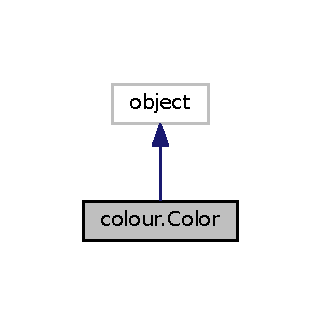
\includegraphics[width=154pt]{classcolour_1_1Color__coll__graph}
\end{center}
\end{figure}
\subsection*{Public Member Functions}
\begin{DoxyCompactItemize}
\item 
\hypertarget{classcolour_1_1Color_acaacc23a6538d6bb8e5327a178bd8ed6}{}def {\bfseries \+\_\+\+\_\+init\+\_\+\+\_\+} (self, \hyperlink{structcolor}{color}=None, pick\+\_\+for=None, picker=R\+G\+B\+\_\+color\+\_\+picker, pick\+\_\+key=hash\+\_\+or\+\_\+str, kwargs)\label{classcolour_1_1Color_acaacc23a6538d6bb8e5327a178bd8ed6}

\item 
\hypertarget{classcolour_1_1Color_a8fff35bebd9fece5a01a7906bd69094e}{}def {\bfseries \+\_\+\+\_\+getattr\+\_\+\+\_\+} (self, label)\label{classcolour_1_1Color_a8fff35bebd9fece5a01a7906bd69094e}

\item 
\hypertarget{classcolour_1_1Color_a63b6606a491b081da36dd350f181870e}{}def {\bfseries \+\_\+\+\_\+setattr\+\_\+\+\_\+} (self, label, value)\label{classcolour_1_1Color_a63b6606a491b081da36dd350f181870e}

\item 
def \hyperlink{classcolour_1_1Color_aa1d8e0def73bf271d12f964609c1eba3}{get\+\_\+hsl} (self)
\begin{DoxyCompactList}\small\item\em Get. \end{DoxyCompactList}\item 
\hypertarget{classcolour_1_1Color_ad8bfc766aa83c37bd115d66f9dce8ffa}{}def {\bfseries get\+\_\+hex} (self)\label{classcolour_1_1Color_ad8bfc766aa83c37bd115d66f9dce8ffa}

\item 
\hypertarget{classcolour_1_1Color_abfdd0669ccebcb69919d21686ab072ab}{}def {\bfseries get\+\_\+hex\+\_\+l} (self)\label{classcolour_1_1Color_abfdd0669ccebcb69919d21686ab072ab}

\item 
\hypertarget{classcolour_1_1Color_a914307dd0d4427bd99a30a888849b42e}{}def {\bfseries get\+\_\+rgb} (self)\label{classcolour_1_1Color_a914307dd0d4427bd99a30a888849b42e}

\item 
\hypertarget{classcolour_1_1Color_a4dd18006c4139d055c2ced25fd9d6dea}{}def {\bfseries get\+\_\+hue} (self)\label{classcolour_1_1Color_a4dd18006c4139d055c2ced25fd9d6dea}

\item 
\hypertarget{classcolour_1_1Color_a1014bb52287cb2916f26c6dec1819710}{}def {\bfseries get\+\_\+saturation} (self)\label{classcolour_1_1Color_a1014bb52287cb2916f26c6dec1819710}

\item 
\hypertarget{classcolour_1_1Color_ae2fdc716be22587cad20486512a8d44b}{}def {\bfseries get\+\_\+luminance} (self)\label{classcolour_1_1Color_ae2fdc716be22587cad20486512a8d44b}

\item 
\hypertarget{classcolour_1_1Color_aa29a66e211aa55ebc21873dc4f472daa}{}def {\bfseries get\+\_\+red} (self)\label{classcolour_1_1Color_aa29a66e211aa55ebc21873dc4f472daa}

\item 
\hypertarget{classcolour_1_1Color_a963f35ade87fb248b23eae30ba90bf82}{}def {\bfseries get\+\_\+green} (self)\label{classcolour_1_1Color_a963f35ade87fb248b23eae30ba90bf82}

\item 
\hypertarget{classcolour_1_1Color_a794cbda47ea884aa2660ea13d96db024}{}def {\bfseries get\+\_\+blue} (self)\label{classcolour_1_1Color_a794cbda47ea884aa2660ea13d96db024}

\item 
\hypertarget{classcolour_1_1Color_ae309c720af12b0eb121feae3e4fb91b4}{}def {\bfseries get\+\_\+web} (self)\label{classcolour_1_1Color_ae309c720af12b0eb121feae3e4fb91b4}

\item 
def \hyperlink{classcolour_1_1Color_afbdfbd7d9c552b56e3532979a1d836a3}{set\+\_\+hsl} (self, value)
\begin{DoxyCompactList}\small\item\em Set. \end{DoxyCompactList}\item 
\hypertarget{classcolour_1_1Color_a8b9b88c7127ceeea8de9f0bf32be4e0e}{}def {\bfseries set\+\_\+rgb} (self, value)\label{classcolour_1_1Color_a8b9b88c7127ceeea8de9f0bf32be4e0e}

\item 
\hypertarget{classcolour_1_1Color_af833ace6170db118a905768147f3bc8e}{}def {\bfseries set\+\_\+hue} (self, value)\label{classcolour_1_1Color_af833ace6170db118a905768147f3bc8e}

\item 
\hypertarget{classcolour_1_1Color_add3ad1b01460b7eeefb4636732c229f5}{}def {\bfseries set\+\_\+saturation} (self, value)\label{classcolour_1_1Color_add3ad1b01460b7eeefb4636732c229f5}

\item 
\hypertarget{classcolour_1_1Color_a5513aae8884037a00bbbaf650c6dcf92}{}def {\bfseries set\+\_\+luminance} (self, value)\label{classcolour_1_1Color_a5513aae8884037a00bbbaf650c6dcf92}

\item 
\hypertarget{classcolour_1_1Color_adee1e689ef93e123576b4e94466bda50}{}def {\bfseries set\+\_\+red} (self, value)\label{classcolour_1_1Color_adee1e689ef93e123576b4e94466bda50}

\item 
\hypertarget{classcolour_1_1Color_ade592872aa8565175e18635a325c57d0}{}def {\bfseries set\+\_\+green} (self, value)\label{classcolour_1_1Color_ade592872aa8565175e18635a325c57d0}

\item 
\hypertarget{classcolour_1_1Color_a2e7a9bae7490ad8475271451041a5e60}{}def {\bfseries set\+\_\+blue} (self, value)\label{classcolour_1_1Color_a2e7a9bae7490ad8475271451041a5e60}

\item 
\hypertarget{classcolour_1_1Color_afa560b9bbcd6ed6bab43260d7860b8f3}{}def {\bfseries set\+\_\+hex} (self, value)\label{classcolour_1_1Color_afa560b9bbcd6ed6bab43260d7860b8f3}

\item 
\hypertarget{classcolour_1_1Color_adca9792fbdce8955d42e9587e071e644}{}def {\bfseries set\+\_\+web} (self, value)\label{classcolour_1_1Color_adca9792fbdce8955d42e9587e071e644}

\item 
def \hyperlink{classcolour_1_1Color_ae3b7a2f7e394802b48ab802fc0795dc5}{range\+\_\+to} (self, value, steps)
\begin{DoxyCompactList}\small\item\em range of color generation \end{DoxyCompactList}\item 
def \hyperlink{classcolour_1_1Color_a31490cb718c0bbd2ae068f94a54545f6}{\+\_\+\+\_\+str\+\_\+\+\_\+} (self)
\begin{DoxyCompactList}\small\item\em Convenience. \end{DoxyCompactList}\item 
\hypertarget{classcolour_1_1Color_aa87bc250985ce54e7ef8c62e343d2e28}{}def {\bfseries \+\_\+\+\_\+repr\+\_\+\+\_\+} (self)\label{classcolour_1_1Color_aa87bc250985ce54e7ef8c62e343d2e28}

\item 
\hypertarget{classcolour_1_1Color_accaec9208b414902d19b88640fe361cb}{}def {\bfseries \+\_\+\+\_\+eq\+\_\+\+\_\+} (self, other)\label{classcolour_1_1Color_accaec9208b414902d19b88640fe361cb}

\end{DoxyCompactItemize}
\subsection*{Public Attributes}
\begin{DoxyCompactItemize}
\item 
\hypertarget{classcolour_1_1Color_a2345c712c9865e6c6a1dbc58bef3d223}{}{\bfseries web}\label{classcolour_1_1Color_a2345c712c9865e6c6a1dbc58bef3d223}

\item 
\hypertarget{classcolour_1_1Color_a5c45a3d98d5c07caf3c5c62000f333c2}{}{\bfseries equality}\label{classcolour_1_1Color_a5c45a3d98d5c07caf3c5c62000f333c2}

\item 
\hypertarget{classcolour_1_1Color_a6beed3d9dcd875668583747c8e3391c6}{}{\bfseries hsl}\label{classcolour_1_1Color_a6beed3d9dcd875668583747c8e3391c6}

\item 
\hypertarget{classcolour_1_1Color_a673b09c77450396516798614b6c8d319}{}{\bfseries rgb}\label{classcolour_1_1Color_a673b09c77450396516798614b6c8d319}

\item 
\hypertarget{classcolour_1_1Color_a15a66e3ea70ace2c23e560f5bb22e49e}{}{\bfseries hex}\label{classcolour_1_1Color_a15a66e3ea70ace2c23e560f5bb22e49e}

\end{DoxyCompactItemize}
\subsection*{Static Public Attributes}
\begin{DoxyCompactItemize}
\item 
\hypertarget{classcolour_1_1Color_a3e7d503337f6c4c7b0395220b02f8bc7}{}{\bfseries set\+\_\+hex\+\_\+l} = set\+\_\+hex\label{classcolour_1_1Color_a3e7d503337f6c4c7b0395220b02f8bc7}

\end{DoxyCompactItemize}
\subsection*{Static Private Attributes}
\begin{DoxyCompactItemize}
\item 
\hypertarget{classcolour_1_1Color_abfa3f6a36a1e85f30908b3733d9e0957}{}{\bfseries \+\_\+hsl} = None\label{classcolour_1_1Color_abfa3f6a36a1e85f30908b3733d9e0957}

\end{DoxyCompactItemize}


\subsection{Detailed Description}
All purpose object. 

\begin{DoxyVerb}Abstraction of a color object

Color object keeps information of a color. It can input/output to different
format (HSL, RGB, HEX, WEB) and their partial representation.

    >>> from colour import Color, HSL

    >>> b = Color()
    >>> b.hsl = HSL.BLUE

Access values
-------------

    >>> b.hue  # doctest: +ELLIPSIS
    0.66...
    >>> b.saturation
    1.0
    >>> b.luminance
    0.5

    >>> b.red
    0.0
    >>> b.blue
    1.0
    >>> b.green
    0.0

    >>> b.rgb
    (0.0, 0.0, 1.0)
    >>> b.hsl  # doctest: +ELLIPSIS
    (0.66..., 1.0, 0.5)
    >>> b.hex
    '#00f'

Change values
-------------

Let's change Hue toward red tint:

    >>> b.hue = 0.0
    >>> b.hex
    '#f00'

    >>> b.hue = 2.0/3
    >>> b.hex
    '#00f'

In the other way round:

    >>> b.hex = '#f00'
    >>> b.hsl
    (0.0, 1.0, 0.5)

Long hex can be accessed directly:

    >>> b.hex_l = '#123456'
    >>> b.hex_l
    '#123456'
    >>> b.hex
    '#123456'

    >>> b.hex_l = '#ff0000'
    >>> b.hex_l
    '#ff0000'
    >>> b.hex
    '#f00'

Convenience
-----------

    >>> c = Color('blue')
    >>> c
    <Color blue>
    >>> c.hue = 0
    >>> c
    <Color red>

    >>> c.saturation = 0.0
    >>> c.hsl  # doctest: +ELLIPSIS
    (..., 0.0, 0.5)
    >>> c.rgb
    (0.5, 0.5, 0.5)
    >>> c.hex
    '#7f7f7f'
    >>> c
    <Color #7f7f7f>

    >>> c.luminance = 0.0
    >>> c
    <Color black>

    >>> c.hex
    '#000'

    >>> c.green = 1.0
    >>> c.blue = 1.0
    >>> c.hex
    '#0ff'
    >>> c
    <Color cyan>

    >>> c = Color('blue', luminance=0.75)
    >>> c
    <Color #7f7fff>

    >>> c = Color('red', red=0.5)
    >>> c
    <Color #7f0000>

    >>> print(c)
    #7f0000

You can try to query unexisting attributes:

    >>> c.lightness  # doctest: +ELLIPSIS
    Traceback (most recent call last):
    ...
    AttributeError: 'lightness' not found

TODO: could add HSV, CMYK, YUV conversion.

#     >>> b.hsv
#     >>> b.value
#     >>> b.cyan
#     >>> b.magenta
#     >>> b.yellow
#     >>> b.key
#     >>> b.cmyk


Recursive init
--------------

To support blind convertion of web strings (or already converted object),
the Color object supports instantiation with another Color object.

    >>> Color(Color(Color('red')))
    <Color red>

Equality support
----------------

Default equality is RGB hex comparison:

    >>> Color('red') == Color('blue')
    False

But this can be changed:

    >>> saturation_equality = lambda c1, c2: c1.luminance == c2.luminance
    >>> Color('red', equality=saturation_equality) == Color('blue')
    True\end{DoxyVerb}
 

\subsection{Member Function Documentation}
\hypertarget{classcolour_1_1Color_a31490cb718c0bbd2ae068f94a54545f6}{}\index{colour\+::\+Color@{colour\+::\+Color}!\+\_\+\+\_\+str\+\_\+\+\_\+@{\+\_\+\+\_\+str\+\_\+\+\_\+}}
\index{\+\_\+\+\_\+str\+\_\+\+\_\+@{\+\_\+\+\_\+str\+\_\+\+\_\+}!colour\+::\+Color@{colour\+::\+Color}}
\subsubsection[{\+\_\+\+\_\+str\+\_\+\+\_\+}]{\setlength{\rightskip}{0pt plus 5cm}def colour.\+Color.\+\_\+\+\_\+str\+\_\+\+\_\+ (
\begin{DoxyParamCaption}
\item[{}]{self}
\end{DoxyParamCaption}
)}\label{classcolour_1_1Color_a31490cb718c0bbd2ae068f94a54545f6}


Convenience. 

\hypertarget{classcolour_1_1Color_aa1d8e0def73bf271d12f964609c1eba3}{}\index{colour\+::\+Color@{colour\+::\+Color}!get\+\_\+hsl@{get\+\_\+hsl}}
\index{get\+\_\+hsl@{get\+\_\+hsl}!colour\+::\+Color@{colour\+::\+Color}}
\subsubsection[{get\+\_\+hsl}]{\setlength{\rightskip}{0pt plus 5cm}def colour.\+Color.\+get\+\_\+hsl (
\begin{DoxyParamCaption}
\item[{}]{self}
\end{DoxyParamCaption}
)}\label{classcolour_1_1Color_aa1d8e0def73bf271d12f964609c1eba3}


Get. 

\hypertarget{classcolour_1_1Color_ae3b7a2f7e394802b48ab802fc0795dc5}{}\index{colour\+::\+Color@{colour\+::\+Color}!range\+\_\+to@{range\+\_\+to}}
\index{range\+\_\+to@{range\+\_\+to}!colour\+::\+Color@{colour\+::\+Color}}
\subsubsection[{range\+\_\+to}]{\setlength{\rightskip}{0pt plus 5cm}def colour.\+Color.\+range\+\_\+to (
\begin{DoxyParamCaption}
\item[{}]{self, }
\item[{}]{value, }
\item[{}]{steps}
\end{DoxyParamCaption}
)}\label{classcolour_1_1Color_ae3b7a2f7e394802b48ab802fc0795dc5}


range of color generation 

\hypertarget{classcolour_1_1Color_afbdfbd7d9c552b56e3532979a1d836a3}{}\index{colour\+::\+Color@{colour\+::\+Color}!set\+\_\+hsl@{set\+\_\+hsl}}
\index{set\+\_\+hsl@{set\+\_\+hsl}!colour\+::\+Color@{colour\+::\+Color}}
\subsubsection[{set\+\_\+hsl}]{\setlength{\rightskip}{0pt plus 5cm}def colour.\+Color.\+set\+\_\+hsl (
\begin{DoxyParamCaption}
\item[{}]{self, }
\item[{}]{value}
\end{DoxyParamCaption}
)}\label{classcolour_1_1Color_afbdfbd7d9c552b56e3532979a1d836a3}


Set. 



The documentation for this class was generated from the following file\+:\begin{DoxyCompactItemize}
\item 
python\+\_\+scripts/colour.\+py\end{DoxyCompactItemize}

\hypertarget{structcolor}{}\section{color Struct Reference}
\label{structcolor}\index{color@{color}}
\subsection*{Public Attributes}
\begin{DoxyCompactItemize}
\item 
\hypertarget{structcolor_a7293811e057a838135d916809d231b05}{}uint8\+\_\+t {\bfseries r}\label{structcolor_a7293811e057a838135d916809d231b05}

\item 
\hypertarget{structcolor_ae81805dcec6033d1efa8e2721baee60e}{}uint8\+\_\+t {\bfseries g}\label{structcolor_ae81805dcec6033d1efa8e2721baee60e}

\item 
\hypertarget{structcolor_a883efd73bb99d3727eceb8bfdd620bc8}{}uint8\+\_\+t {\bfseries b}\label{structcolor_a883efd73bb99d3727eceb8bfdd620bc8}

\end{DoxyCompactItemize}


The documentation for this struct was generated from the following file\+:\begin{DoxyCompactItemize}
\item 
src/led.\+h\end{DoxyCompactItemize}

\hypertarget{structfilter__rms}{}\section{filter\+\_\+rms Struct Reference}
\label{structfilter__rms}\index{filter\+\_\+rms@{filter\+\_\+rms}}


Collaboration diagram for filter\+\_\+rms\+:\nopagebreak
\begin{figure}[H]
\begin{center}
\leavevmode
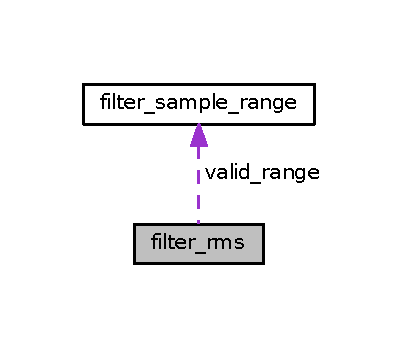
\includegraphics[width=194pt]{structfilter__rms__coll__graph}
\end{center}
\end{figure}
\subsection*{Public Attributes}
\begin{DoxyCompactItemize}
\item 
\hypertarget{structfilter__rms_a54520c4d0cb0f9441f4c57eacf5bfd78}{}volatile uint32\+\_\+t $\ast$ {\bfseries buffer}\label{structfilter__rms_a54520c4d0cb0f9441f4c57eacf5bfd78}

\item 
\hypertarget{structfilter__rms_a8581be35641ea200e6bf23ce48f76196}{}uint32\+\_\+t {\bfseries size}\label{structfilter__rms_a8581be35641ea200e6bf23ce48f76196}

\item 
\hypertarget{structfilter__rms_a85d467406ed373c2ad1a134860fd24bd}{}int {\bfseries pos}\label{structfilter__rms_a85d467406ed373c2ad1a134860fd24bd}

\item 
\hypertarget{structfilter__rms_a42976cc476c577216f312bcd496eb79b}{}uint32\+\_\+t {\bfseries count}\label{structfilter__rms_a42976cc476c577216f312bcd496eb79b}

\item 
\hypertarget{structfilter__rms_a902e6aa671bf468ba0506ef5848f51cf}{}uint32\+\_\+t {\bfseries sqsum}\label{structfilter__rms_a902e6aa671bf468ba0506ef5848f51cf}

\item 
\hypertarget{structfilter__rms_a00a96dc7cf61e9c2643fdefc3d558ff2}{}int {\bfseries invalid\+\_\+samples\+\_\+streak}\label{structfilter__rms_a00a96dc7cf61e9c2643fdefc3d558ff2}

\item 
\hypertarget{structfilter__rms_abcd2a21aa49c2abb148493265da1efa5}{}struct \hyperlink{structfilter__sample__range}{filter\+\_\+sample\+\_\+range} {\bfseries valid\+\_\+range}\label{structfilter__rms_abcd2a21aa49c2abb148493265da1efa5}

\end{DoxyCompactItemize}


The documentation for this struct was generated from the following file\+:\begin{DoxyCompactItemize}
\item 
src/filter.\+h\end{DoxyCompactItemize}

\hypertarget{structfilter__sample__range}{}\section{filter\+\_\+sample\+\_\+range Struct Reference}
\label{structfilter__sample__range}\index{filter\+\_\+sample\+\_\+range@{filter\+\_\+sample\+\_\+range}}
\subsection*{Public Attributes}
\begin{DoxyCompactItemize}
\item 
\hypertarget{structfilter__sample__range_a304ee67b1a15b4a0f36ca190a56a38c7}{}int {\bfseries min}\label{structfilter__sample__range_a304ee67b1a15b4a0f36ca190a56a38c7}

\item 
\hypertarget{structfilter__sample__range_a0a29f8303981c999d499070d0a05e05d}{}int {\bfseries max}\label{structfilter__sample__range_a0a29f8303981c999d499070d0a05e05d}

\end{DoxyCompactItemize}


The documentation for this struct was generated from the following file\+:\begin{DoxyCompactItemize}
\item 
src/filter.\+h\end{DoxyCompactItemize}

\hypertarget{structgpio__pin}{}\section{gpio\+\_\+pin Struct Reference}
\label{structgpio__pin}\index{gpio\+\_\+pin@{gpio\+\_\+pin}}


Collaboration diagram for gpio\+\_\+pin\+:\nopagebreak
\begin{figure}[H]
\begin{center}
\leavevmode
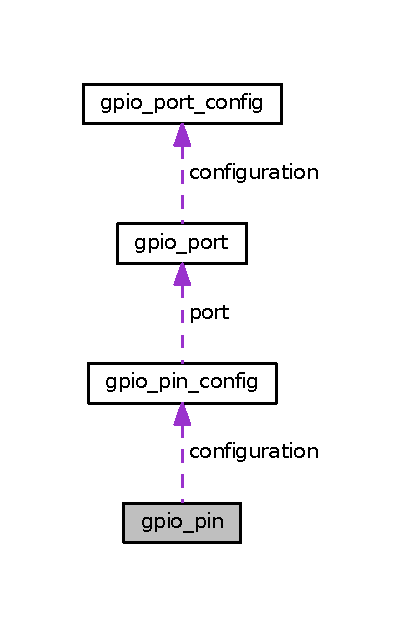
\includegraphics[width=194pt]{structgpio__pin__coll__graph}
\end{center}
\end{figure}
\subsection*{Public Attributes}
\begin{DoxyCompactItemize}
\item 
\hypertarget{structgpio__pin_acb6a2426999aa0f3e40d37a02f791e75}{}struct \hyperlink{structgpio__pin__config}{gpio\+\_\+pin\+\_\+config} $\ast$ {\bfseries configuration}\label{structgpio__pin_acb6a2426999aa0f3e40d37a02f791e75}

\item 
\hypertarget{structgpio__pin_a4d4c7f491d051331985524f88f81fa58}{}enum \hyperlink{hw_8h_a3c02952100e7d051b77cdf060ca0ba9b}{hw\+\_\+init\+\_\+state} {\bfseries state}\label{structgpio__pin_a4d4c7f491d051331985524f88f81fa58}

\end{DoxyCompactItemize}


The documentation for this struct was generated from the following file\+:\begin{DoxyCompactItemize}
\item 
src/gpio.\+h\end{DoxyCompactItemize}

\hypertarget{structgpio__pin__config}{}\section{gpio\+\_\+pin\+\_\+config Struct Reference}
\label{structgpio__pin__config}\index{gpio\+\_\+pin\+\_\+config@{gpio\+\_\+pin\+\_\+config}}


Collaboration diagram for gpio\+\_\+pin\+\_\+config\+:\nopagebreak
\begin{figure}[H]
\begin{center}
\leavevmode
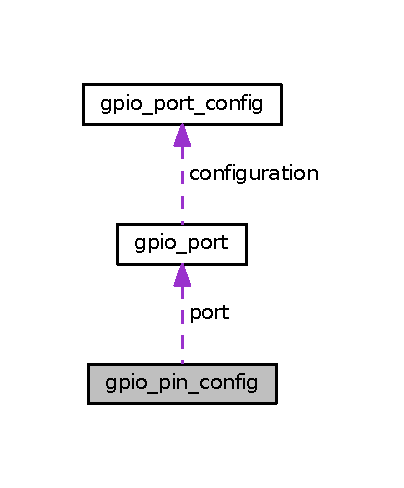
\includegraphics[width=194pt]{structgpio__pin__config__coll__graph}
\end{center}
\end{figure}
\subsection*{Public Attributes}
\begin{DoxyCompactItemize}
\item 
\hypertarget{structgpio__pin__config_a72fc1227f3fab0d1e2485d8f4bed6dbc}{}struct \hyperlink{structgpio__port}{gpio\+\_\+port} $\ast$ {\bfseries port}\label{structgpio__pin__config_a72fc1227f3fab0d1e2485d8f4bed6dbc}

\item 
\hypertarget{structgpio__pin__config_afb9b5bbf5c85e22120e7ef67964b621a}{}uint32\+\_\+t {\bfseries pin}\label{structgpio__pin__config_afb9b5bbf5c85e22120e7ef67964b621a}

\item 
\hypertarget{structgpio__pin__config_a799cc96abd94ffdc23f888a9ed1556ca}{}uint32\+\_\+t {\bfseries mode}\label{structgpio__pin__config_a799cc96abd94ffdc23f888a9ed1556ca}

\item 
\hypertarget{structgpio__pin__config_a1ba8ae193e2164dd8c4238c81d9200e4}{}uint32\+\_\+t {\bfseries configuration}\label{structgpio__pin__config_a1ba8ae193e2164dd8c4238c81d9200e4}

\item 
\hypertarget{structgpio__pin__config_a195076654c4665c2dae2702f4bce5dfd}{}int {\bfseries initial}\label{structgpio__pin__config_a195076654c4665c2dae2702f4bce5dfd}

\end{DoxyCompactItemize}


The documentation for this struct was generated from the following file\+:\begin{DoxyCompactItemize}
\item 
src/gpio.\+h\end{DoxyCompactItemize}

\hypertarget{structgpio__port}{}\section{gpio\+\_\+port Struct Reference}
\label{structgpio__port}\index{gpio\+\_\+port@{gpio\+\_\+port}}


Collaboration diagram for gpio\+\_\+port\+:\nopagebreak
\begin{figure}[H]
\begin{center}
\leavevmode
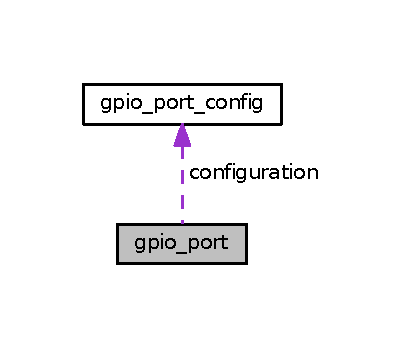
\includegraphics[width=194pt]{structgpio__port__coll__graph}
\end{center}
\end{figure}
\subsection*{Public Attributes}
\begin{DoxyCompactItemize}
\item 
\hypertarget{structgpio__port_ad67106287ff2c5d84c528b731374d5e8}{}struct \hyperlink{structgpio__port__config}{gpio\+\_\+port\+\_\+config} $\ast$ {\bfseries configuration}\label{structgpio__port_ad67106287ff2c5d84c528b731374d5e8}

\item 
\hypertarget{structgpio__port_acc0ba075ca33d19af55b06b16edd7ac6}{}enum \hyperlink{hw_8h_a3c02952100e7d051b77cdf060ca0ba9b}{hw\+\_\+init\+\_\+state} {\bfseries state}\label{structgpio__port_acc0ba075ca33d19af55b06b16edd7ac6}

\end{DoxyCompactItemize}


The documentation for this struct was generated from the following file\+:\begin{DoxyCompactItemize}
\item 
src/gpio.\+h\end{DoxyCompactItemize}

\hypertarget{structgpio__port__config}{}\section{gpio\+\_\+port\+\_\+config Struct Reference}
\label{structgpio__port__config}\index{gpio\+\_\+port\+\_\+config@{gpio\+\_\+port\+\_\+config}}
\subsection*{Public Attributes}
\begin{DoxyCompactItemize}
\item 
\hypertarget{structgpio__port__config_a37f5f40d14a183161a8dd4fd9ede9d05}{}uint32\+\_\+t {\bfseries port}\label{structgpio__port__config_a37f5f40d14a183161a8dd4fd9ede9d05}

\item 
\hypertarget{structgpio__port__config_a00cb058b3750f38e4b3c5be01e9b0f25}{}uint32\+\_\+t {\bfseries rcc}\label{structgpio__port__config_a00cb058b3750f38e4b3c5be01e9b0f25}

\end{DoxyCompactItemize}


The documentation for this struct was generated from the following file\+:\begin{DoxyCompactItemize}
\item 
src/gpio.\+h\end{DoxyCompactItemize}

\hypertarget{classcolour_1_1HSL}{}\section{colour.\+H\+S\+L Class Reference}
\label{classcolour_1_1HSL}\index{colour.\+H\+S\+L@{colour.\+H\+S\+L}}
\subsection*{Static Public Attributes}
\begin{DoxyCompactItemize}
\item 
\hypertarget{classcolour_1_1HSL_a126535ecb96c65c30fe3e45a15047877}{}tuple {\bfseries B\+L\+A\+C\+K} = (0.\+0 , 0.\+0, 0.\+0)\label{classcolour_1_1HSL_a126535ecb96c65c30fe3e45a15047877}

\item 
\hypertarget{classcolour_1_1HSL_a58cd85479743c70f8dc3655057b3dfda}{}tuple {\bfseries W\+H\+I\+T\+E} = (0.\+0 , 0.\+0, 1.\+0)\label{classcolour_1_1HSL_a58cd85479743c70f8dc3655057b3dfda}

\item 
\hypertarget{classcolour_1_1HSL_aeeb08d5ae80e34d8e7dcbd4e8df43ace}{}tuple {\bfseries R\+E\+D} = (0.\+0 , 1.\+0, 0.\+5)\label{classcolour_1_1HSL_aeeb08d5ae80e34d8e7dcbd4e8df43ace}

\item 
\hypertarget{classcolour_1_1HSL_af8bd1775a12264c0dc5d721fc9334575}{}tuple {\bfseries G\+R\+E\+E\+N} = (1.\+0/3, 1.\+0, 0.\+5)\label{classcolour_1_1HSL_af8bd1775a12264c0dc5d721fc9334575}

\item 
\hypertarget{classcolour_1_1HSL_af331e70dfb1f8dd5679b71e33dfd2827}{}tuple {\bfseries B\+L\+U\+E} = (2.\+0/3, 1.\+0, 0.\+5)\label{classcolour_1_1HSL_af331e70dfb1f8dd5679b71e33dfd2827}

\item 
\hypertarget{classcolour_1_1HSL_abe816fe43dce26a94ab583a1b4f4ea47}{}tuple {\bfseries G\+R\+A\+Y} = (0.\+0 , 0.\+0, 0.\+5)\label{classcolour_1_1HSL_abe816fe43dce26a94ab583a1b4f4ea47}

\end{DoxyCompactItemize}


The documentation for this class was generated from the following file\+:\begin{DoxyCompactItemize}
\item 
python\+\_\+scripts/colour.\+py\end{DoxyCompactItemize}

\hypertarget{structirrigation__controller}{}\section{irrigation\+\_\+controller Struct Reference}
\label{structirrigation__controller}\index{irrigation\+\_\+controller@{irrigation\+\_\+controller}}


Holds everything related to the irrigation controller.  




{\ttfamily \#include $<$irrigation.\+h$>$}



Collaboration diagram for irrigation\+\_\+controller\+:\nopagebreak
\begin{figure}[H]
\begin{center}
\leavevmode
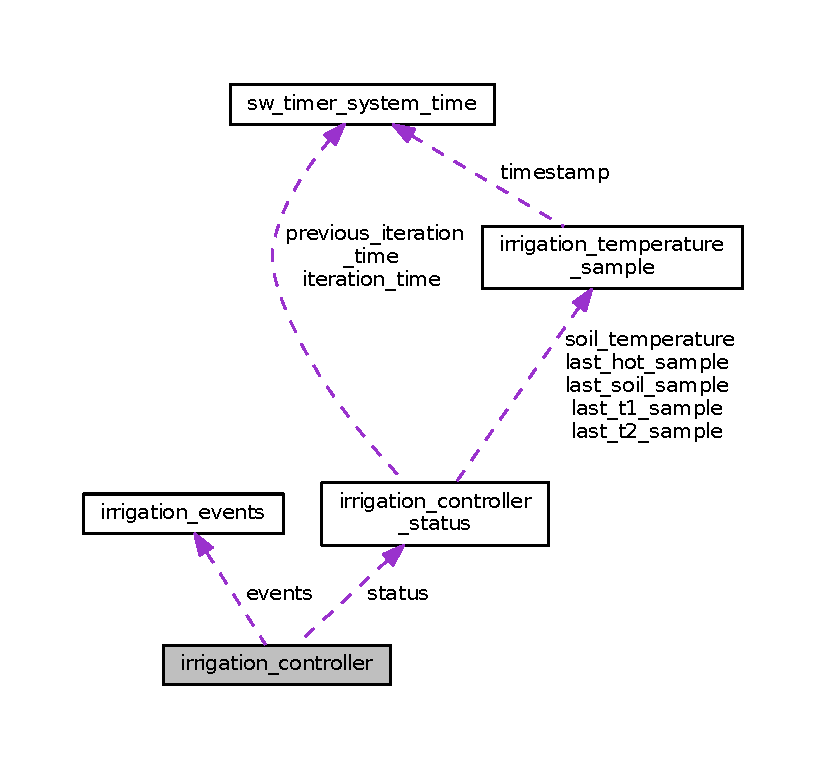
\includegraphics[width=350pt]{structirrigation__controller__coll__graph}
\end{center}
\end{figure}
\subsection*{Public Attributes}
\begin{DoxyCompactItemize}
\item 
struct \hyperlink{structirrigation__controller__status}{irrigation\+\_\+controller\+\_\+status} \hyperlink{structirrigation__controller_a68a854df15c9234d24f2ad36b990bfa8}{status}
\begin{DoxyCompactList}\small\item\em Status and measurements. \end{DoxyCompactList}\item 
enum \hyperlink{irrigation_8h_ac40bd72ec6942e213e454ebcacc92dc7}{irrigation\+\_\+status} \hyperlink{structirrigation__controller_a80bec16de2d6f98564ed1487dee041c5}{current\+\_\+state}
\begin{DoxyCompactList}\small\item\em Current state in the \hyperlink{group__state__machine}{The main state machine}. \end{DoxyCompactList}\item 
enum \hyperlink{irrigation_8h_ac40bd72ec6942e213e454ebcacc92dc7}{irrigation\+\_\+status} \hyperlink{structirrigation__controller_a7e1c5689983d2b8aae434c2d5442c935}{pending\+\_\+state}
\begin{DoxyCompactList}\small\item\em Pending state in the \hyperlink{group__state__machine}{The main state machine}. \end{DoxyCompactList}\item 
\hypertarget{structirrigation__controller_a4ae62413005c2121bee0ac25a0119cbc}{}struct \hyperlink{structirrigation__events}{irrigation\+\_\+events} {\bfseries events}\label{structirrigation__controller_a4ae62413005c2121bee0ac25a0119cbc}

\item 
\hypertarget{structirrigation__controller_a94cb4b4c26de9f40543f06335afa036c}{}int {\bfseries heater}\label{structirrigation__controller_a94cb4b4c26de9f40543f06335afa036c}

\item 
\hypertarget{structirrigation__controller_a38217da0082898392465f4ee2901f73b}{}int {\bfseries pump}\label{structirrigation__controller_a38217da0082898392465f4ee2901f73b}

\end{DoxyCompactItemize}


\subsection{Detailed Description}
Holds everything related to the irrigation controller. 

\subsection{Member Data Documentation}
\hypertarget{structirrigation__controller_a80bec16de2d6f98564ed1487dee041c5}{}\index{irrigation\+\_\+controller@{irrigation\+\_\+controller}!current\+\_\+state@{current\+\_\+state}}
\index{current\+\_\+state@{current\+\_\+state}!irrigation\+\_\+controller@{irrigation\+\_\+controller}}
\subsubsection[{current\+\_\+state}]{\setlength{\rightskip}{0pt plus 5cm}enum {\bf irrigation\+\_\+status} irrigation\+\_\+controller\+::current\+\_\+state}\label{structirrigation__controller_a80bec16de2d6f98564ed1487dee041c5}


Current state in the \hyperlink{group__state__machine}{The main state machine}. 

\hypertarget{structirrigation__controller_a7e1c5689983d2b8aae434c2d5442c935}{}\index{irrigation\+\_\+controller@{irrigation\+\_\+controller}!pending\+\_\+state@{pending\+\_\+state}}
\index{pending\+\_\+state@{pending\+\_\+state}!irrigation\+\_\+controller@{irrigation\+\_\+controller}}
\subsubsection[{pending\+\_\+state}]{\setlength{\rightskip}{0pt plus 5cm}enum {\bf irrigation\+\_\+status} irrigation\+\_\+controller\+::pending\+\_\+state}\label{structirrigation__controller_a7e1c5689983d2b8aae434c2d5442c935}


Pending state in the \hyperlink{group__state__machine}{The main state machine}. 

\hypertarget{structirrigation__controller_a68a854df15c9234d24f2ad36b990bfa8}{}\index{irrigation\+\_\+controller@{irrigation\+\_\+controller}!status@{status}}
\index{status@{status}!irrigation\+\_\+controller@{irrigation\+\_\+controller}}
\subsubsection[{status}]{\setlength{\rightskip}{0pt plus 5cm}struct {\bf irrigation\+\_\+controller\+\_\+status} irrigation\+\_\+controller\+::status}\label{structirrigation__controller_a68a854df15c9234d24f2ad36b990bfa8}


Status and measurements. 



The documentation for this struct was generated from the following file\+:\begin{DoxyCompactItemize}
\item 
src/\hyperlink{irrigation_8h}{irrigation.\+h}\end{DoxyCompactItemize}

\hypertarget{structirrigation__controller__status}{}\section{irrigation\+\_\+controller\+\_\+status Struct Reference}
\label{structirrigation__controller__status}\index{irrigation\+\_\+controller\+\_\+status@{irrigation\+\_\+controller\+\_\+status}}


Collaboration diagram for irrigation\+\_\+controller\+\_\+status\+:\nopagebreak
\begin{figure}[H]
\begin{center}
\leavevmode
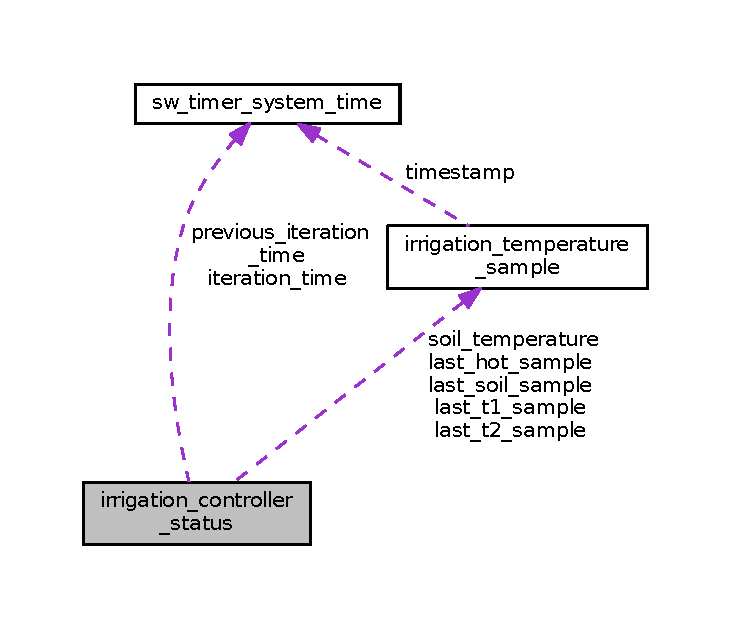
\includegraphics[width=350pt]{structirrigation__controller__status__coll__graph}
\end{center}
\end{figure}
\subsection*{Public Attributes}
\begin{DoxyCompactItemize}
\item 
float \hyperlink{structirrigation__controller__status_a0a4447a8aa2200bacf97bd7e844493c1}{dt}
\begin{DoxyCompactList}\small\item\em Delta time since last state run. \end{DoxyCompactList}\item 
struct \hyperlink{structsw__timer__system__time}{sw\+\_\+timer\+\_\+system\+\_\+time} \hyperlink{structirrigation__controller__status_a1ae5ffb12725754d8309452cf24a2a28}{iteration\+\_\+time}
\begin{DoxyCompactList}\small\item\em Timestamp of when this run started. \end{DoxyCompactList}\item 
struct \hyperlink{structsw__timer__system__time}{sw\+\_\+timer\+\_\+system\+\_\+time} \hyperlink{structirrigation__controller__status_ab5a5ed310a96d8fd4db605bad57bf83a}{previous\+\_\+iteration\+\_\+time}
\begin{DoxyCompactList}\small\item\em Timestamp of previous run, used to calculate \hyperlink{structirrigation__controller__status_a0a4447a8aa2200bacf97bd7e844493c1}{dt}. \end{DoxyCompactList}\item 
\hypertarget{structirrigation__controller__status_a113b7e81a993c20bb5bf90b2faf81bc5}{}enum \hyperlink{irrigation_8h_a9891f6b3b37611d2aebdb8601acdf6c6}{moisture\+\_\+sensor\+\_\+state} {\bfseries sensor\+\_\+state}\label{structirrigation__controller__status_a113b7e81a993c20bb5bf90b2faf81bc5}

\item 
\hypertarget{structirrigation__controller__status_a9f6f7c1cab26fb9200e9ab706098cb98}{}float {\bfseries ackumulative\+\_\+delta\+\_\+temp}\label{structirrigation__controller__status_a9f6f7c1cab26fb9200e9ab706098cb98}

\item 
\hypertarget{structirrigation__controller__status_a6b0753e3ea72f0220cb51e9e14d817ba}{}float {\bfseries ackumulative\+\_\+delta\+\_\+time}\label{structirrigation__controller__status_a6b0753e3ea72f0220cb51e9e14d817ba}

\item 
\hypertarget{structirrigation__controller__status_ae84f5b8517b8fe266305aa248a6f46fc}{}float {\bfseries heating\+\_\+time}\label{structirrigation__controller__status_ae84f5b8517b8fe266305aa248a6f46fc}

\item 
\hypertarget{structirrigation__controller__status_a7b67f38b1433b1909b3afc32fe6b22d9}{}float {\bfseries cooling\+\_\+time}\label{structirrigation__controller__status_a7b67f38b1433b1909b3afc32fe6b22d9}

\item 
struct \hyperlink{structirrigation__temperature__sample}{irrigation\+\_\+temperature\+\_\+sample} \hyperlink{structirrigation__controller__status_a3ef3b031a2c91413170ad02626e8da1c}{soil\+\_\+temperature}
\begin{DoxyCompactList}\small\item\em Last soil temperature measured. \end{DoxyCompactList}\item 
struct \hyperlink{structirrigation__temperature__sample}{irrigation\+\_\+temperature\+\_\+sample} \hyperlink{structirrigation__controller__status_a2d3ef640dc3ec8ce2789fffb092d8f80}{last\+\_\+soil\+\_\+sample}
\begin{DoxyCompactList}\small\item\em Holds the temperature of an initial water content sampling. \end{DoxyCompactList}\item 
struct \hyperlink{structirrigation__temperature__sample}{irrigation\+\_\+temperature\+\_\+sample} \hyperlink{structirrigation__controller__status_ab795e232c4e2d405b11e24312a6163c3}{last\+\_\+hot\+\_\+sample}
\item 
\hypertarget{structirrigation__controller__status_a9b64c69b881c0befd37f25d81141ae24}{}struct \hyperlink{structirrigation__temperature__sample}{irrigation\+\_\+temperature\+\_\+sample} {\bfseries last\+\_\+t1\+\_\+sample}\label{structirrigation__controller__status_a9b64c69b881c0befd37f25d81141ae24}

\item 
\hypertarget{structirrigation__controller__status_af481460c8a71385556ae6a336245fb89}{}struct \hyperlink{structirrigation__temperature__sample}{irrigation\+\_\+temperature\+\_\+sample} {\bfseries last\+\_\+t2\+\_\+sample}\label{structirrigation__controller__status_af481460c8a71385556ae6a336245fb89}

\item 
float \hyperlink{structirrigation__controller__status_a451e58983d5995bf6f1e00f9318d5dd6}{min\+\_\+temperature}
\begin{DoxyCompactList}\small\item\em This is the minimum temperature during \hyperlink{group__state__validate}{Sensor validation state}. \end{DoxyCompactList}\item 
float \hyperlink{structirrigation__controller__status_a1bd8f83a44ee01d3b7cf3851b6716f02}{max\+\_\+temperature}
\begin{DoxyCompactList}\small\item\em This is the minimum temperature during \hyperlink{group__state__validate}{Sensor validation state}. \end{DoxyCompactList}\item 
float \hyperlink{structirrigation__controller__status_a360e7ee7f6ac54635fc66035883d2d9c}{validation\+\_\+timer}
\begin{DoxyCompactList}\small\item\em This is the timer for \hyperlink{group__state__validate}{Sensor validation state}. \end{DoxyCompactList}\item 
float \hyperlink{structirrigation__controller__status_a9d70c74fe395ec2720089b929a32e1e9}{initial\+\_\+timer}
\begin{DoxyCompactList}\small\item\em This is the timer for \hyperlink{group__state__init}{Initial state}. \end{DoxyCompactList}\item 
float \hyperlink{structirrigation__controller__status_aab428bb9e677098d336aefd32b5e6232}{periodic\+\_\+temp\+\_\+report}
\begin{DoxyCompactList}\small\item\em This is a timer for periodic calls to \hyperlink{structirrigation__events_a47b81edd52377b4c4e1ed512b830e237}{irrigation\+\_\+events\+::report\+\_\+current\+\_\+temperature}. \end{DoxyCompactList}\end{DoxyCompactItemize}


\subsection{Member Data Documentation}
\hypertarget{structirrigation__controller__status_a0a4447a8aa2200bacf97bd7e844493c1}{}\index{irrigation\+\_\+controller\+\_\+status@{irrigation\+\_\+controller\+\_\+status}!dt@{dt}}
\index{dt@{dt}!irrigation\+\_\+controller\+\_\+status@{irrigation\+\_\+controller\+\_\+status}}
\subsubsection[{dt}]{\setlength{\rightskip}{0pt plus 5cm}float irrigation\+\_\+controller\+\_\+status\+::dt}\label{structirrigation__controller__status_a0a4447a8aa2200bacf97bd7e844493c1}


Delta time since last state run. 

\hypertarget{structirrigation__controller__status_a9d70c74fe395ec2720089b929a32e1e9}{}\index{irrigation\+\_\+controller\+\_\+status@{irrigation\+\_\+controller\+\_\+status}!initial\+\_\+timer@{initial\+\_\+timer}}
\index{initial\+\_\+timer@{initial\+\_\+timer}!irrigation\+\_\+controller\+\_\+status@{irrigation\+\_\+controller\+\_\+status}}
\subsubsection[{initial\+\_\+timer}]{\setlength{\rightskip}{0pt plus 5cm}float irrigation\+\_\+controller\+\_\+status\+::initial\+\_\+timer}\label{structirrigation__controller__status_a9d70c74fe395ec2720089b929a32e1e9}


This is the timer for \hyperlink{group__state__init}{Initial state}. 

\hypertarget{structirrigation__controller__status_a1ae5ffb12725754d8309452cf24a2a28}{}\index{irrigation\+\_\+controller\+\_\+status@{irrigation\+\_\+controller\+\_\+status}!iteration\+\_\+time@{iteration\+\_\+time}}
\index{iteration\+\_\+time@{iteration\+\_\+time}!irrigation\+\_\+controller\+\_\+status@{irrigation\+\_\+controller\+\_\+status}}
\subsubsection[{iteration\+\_\+time}]{\setlength{\rightskip}{0pt plus 5cm}struct {\bf sw\+\_\+timer\+\_\+system\+\_\+time} irrigation\+\_\+controller\+\_\+status\+::iteration\+\_\+time}\label{structirrigation__controller__status_a1ae5ffb12725754d8309452cf24a2a28}


Timestamp of when this run started. 

\hypertarget{structirrigation__controller__status_ab795e232c4e2d405b11e24312a6163c3}{}\index{irrigation\+\_\+controller\+\_\+status@{irrigation\+\_\+controller\+\_\+status}!last\+\_\+hot\+\_\+sample@{last\+\_\+hot\+\_\+sample}}
\index{last\+\_\+hot\+\_\+sample@{last\+\_\+hot\+\_\+sample}!irrigation\+\_\+controller\+\_\+status@{irrigation\+\_\+controller\+\_\+status}}
\subsubsection[{last\+\_\+hot\+\_\+sample}]{\setlength{\rightskip}{0pt plus 5cm}struct {\bf irrigation\+\_\+temperature\+\_\+sample} irrigation\+\_\+controller\+\_\+status\+::last\+\_\+hot\+\_\+sample}\label{structirrigation__controller__status_ab795e232c4e2d405b11e24312a6163c3}
\begin{DoxyRefDesc}{Todo}
\item[\hyperlink{todo__todo000004}{Todo}]Clean up unused stuff here \end{DoxyRefDesc}
\hypertarget{structirrigation__controller__status_a2d3ef640dc3ec8ce2789fffb092d8f80}{}\index{irrigation\+\_\+controller\+\_\+status@{irrigation\+\_\+controller\+\_\+status}!last\+\_\+soil\+\_\+sample@{last\+\_\+soil\+\_\+sample}}
\index{last\+\_\+soil\+\_\+sample@{last\+\_\+soil\+\_\+sample}!irrigation\+\_\+controller\+\_\+status@{irrigation\+\_\+controller\+\_\+status}}
\subsubsection[{last\+\_\+soil\+\_\+sample}]{\setlength{\rightskip}{0pt plus 5cm}struct {\bf irrigation\+\_\+temperature\+\_\+sample} irrigation\+\_\+controller\+\_\+status\+::last\+\_\+soil\+\_\+sample}\label{structirrigation__controller__status_a2d3ef640dc3ec8ce2789fffb092d8f80}


Holds the temperature of an initial water content sampling. 

\hypertarget{structirrigation__controller__status_a1bd8f83a44ee01d3b7cf3851b6716f02}{}\index{irrigation\+\_\+controller\+\_\+status@{irrigation\+\_\+controller\+\_\+status}!max\+\_\+temperature@{max\+\_\+temperature}}
\index{max\+\_\+temperature@{max\+\_\+temperature}!irrigation\+\_\+controller\+\_\+status@{irrigation\+\_\+controller\+\_\+status}}
\subsubsection[{max\+\_\+temperature}]{\setlength{\rightskip}{0pt plus 5cm}float irrigation\+\_\+controller\+\_\+status\+::max\+\_\+temperature}\label{structirrigation__controller__status_a1bd8f83a44ee01d3b7cf3851b6716f02}


This is the minimum temperature during \hyperlink{group__state__validate}{Sensor validation state}. 

\hypertarget{structirrigation__controller__status_a451e58983d5995bf6f1e00f9318d5dd6}{}\index{irrigation\+\_\+controller\+\_\+status@{irrigation\+\_\+controller\+\_\+status}!min\+\_\+temperature@{min\+\_\+temperature}}
\index{min\+\_\+temperature@{min\+\_\+temperature}!irrigation\+\_\+controller\+\_\+status@{irrigation\+\_\+controller\+\_\+status}}
\subsubsection[{min\+\_\+temperature}]{\setlength{\rightskip}{0pt plus 5cm}float irrigation\+\_\+controller\+\_\+status\+::min\+\_\+temperature}\label{structirrigation__controller__status_a451e58983d5995bf6f1e00f9318d5dd6}


This is the minimum temperature during \hyperlink{group__state__validate}{Sensor validation state}. 

\hypertarget{structirrigation__controller__status_aab428bb9e677098d336aefd32b5e6232}{}\index{irrigation\+\_\+controller\+\_\+status@{irrigation\+\_\+controller\+\_\+status}!periodic\+\_\+temp\+\_\+report@{periodic\+\_\+temp\+\_\+report}}
\index{periodic\+\_\+temp\+\_\+report@{periodic\+\_\+temp\+\_\+report}!irrigation\+\_\+controller\+\_\+status@{irrigation\+\_\+controller\+\_\+status}}
\subsubsection[{periodic\+\_\+temp\+\_\+report}]{\setlength{\rightskip}{0pt plus 5cm}float irrigation\+\_\+controller\+\_\+status\+::periodic\+\_\+temp\+\_\+report}\label{structirrigation__controller__status_aab428bb9e677098d336aefd32b5e6232}


This is a timer for periodic calls to \hyperlink{structirrigation__events_a47b81edd52377b4c4e1ed512b830e237}{irrigation\+\_\+events\+::report\+\_\+current\+\_\+temperature}. 

\hypertarget{structirrigation__controller__status_ab5a5ed310a96d8fd4db605bad57bf83a}{}\index{irrigation\+\_\+controller\+\_\+status@{irrigation\+\_\+controller\+\_\+status}!previous\+\_\+iteration\+\_\+time@{previous\+\_\+iteration\+\_\+time}}
\index{previous\+\_\+iteration\+\_\+time@{previous\+\_\+iteration\+\_\+time}!irrigation\+\_\+controller\+\_\+status@{irrigation\+\_\+controller\+\_\+status}}
\subsubsection[{previous\+\_\+iteration\+\_\+time}]{\setlength{\rightskip}{0pt plus 5cm}struct {\bf sw\+\_\+timer\+\_\+system\+\_\+time} irrigation\+\_\+controller\+\_\+status\+::previous\+\_\+iteration\+\_\+time}\label{structirrigation__controller__status_ab5a5ed310a96d8fd4db605bad57bf83a}


Timestamp of previous run, used to calculate \hyperlink{structirrigation__controller__status_a0a4447a8aa2200bacf97bd7e844493c1}{dt}. 

\hypertarget{structirrigation__controller__status_a3ef3b031a2c91413170ad02626e8da1c}{}\index{irrigation\+\_\+controller\+\_\+status@{irrigation\+\_\+controller\+\_\+status}!soil\+\_\+temperature@{soil\+\_\+temperature}}
\index{soil\+\_\+temperature@{soil\+\_\+temperature}!irrigation\+\_\+controller\+\_\+status@{irrigation\+\_\+controller\+\_\+status}}
\subsubsection[{soil\+\_\+temperature}]{\setlength{\rightskip}{0pt plus 5cm}struct {\bf irrigation\+\_\+temperature\+\_\+sample} irrigation\+\_\+controller\+\_\+status\+::soil\+\_\+temperature}\label{structirrigation__controller__status_a3ef3b031a2c91413170ad02626e8da1c}


Last soil temperature measured. 

\hypertarget{structirrigation__controller__status_a360e7ee7f6ac54635fc66035883d2d9c}{}\index{irrigation\+\_\+controller\+\_\+status@{irrigation\+\_\+controller\+\_\+status}!validation\+\_\+timer@{validation\+\_\+timer}}
\index{validation\+\_\+timer@{validation\+\_\+timer}!irrigation\+\_\+controller\+\_\+status@{irrigation\+\_\+controller\+\_\+status}}
\subsubsection[{validation\+\_\+timer}]{\setlength{\rightskip}{0pt plus 5cm}float irrigation\+\_\+controller\+\_\+status\+::validation\+\_\+timer}\label{structirrigation__controller__status_a360e7ee7f6ac54635fc66035883d2d9c}


This is the timer for \hyperlink{group__state__validate}{Sensor validation state}. 



The documentation for this struct was generated from the following file\+:\begin{DoxyCompactItemize}
\item 
src/\hyperlink{irrigation_8h}{irrigation.\+h}\end{DoxyCompactItemize}

\hypertarget{structirrigation__events}{}\section{irrigation\+\_\+events Struct Reference}
\label{structirrigation__events}\index{irrigation\+\_\+events@{irrigation\+\_\+events}}


The event callback functions for the irrigation controller core.  




{\ttfamily \#include $<$irrigation.\+h$>$}

\subsection*{Public Attributes}
\begin{DoxyCompactItemize}
\item 
void($\ast$ \hyperlink{structirrigation__events_acc5d9d31cce6888cab54d32463470f07}{report\+\_\+validation\+\_\+temperatures} )(struct \hyperlink{structirrigation__controller}{irrigation\+\_\+controller} $\ast$)
\begin{DoxyCompactList}\small\item\em Report the measured temperatures for validation. \end{DoxyCompactList}\item 
void($\ast$ \hyperlink{structirrigation__events_abafd6872889e6e54648653f690e61ec6}{report\+\_\+sensor\+\_\+malfunction} )(struct \hyperlink{structirrigation__controller}{irrigation\+\_\+controller} $\ast$)
\begin{DoxyCompactList}\small\item\em Report that sensordata is invalid. \end{DoxyCompactList}\item 
void($\ast$ \hyperlink{structirrigation__events_a41db6d6a624689abdb7be82425ff0b02}{report\+\_\+sensor\+\_\+fluctuations} )(struct \hyperlink{structirrigation__controller}{irrigation\+\_\+controller} $\ast$)
\begin{DoxyCompactList}\small\item\em Report that sensordata fluctuates. \end{DoxyCompactList}\item 
void($\ast$ \hyperlink{structirrigation__events_a47b81edd52377b4c4e1ed512b830e237}{report\+\_\+current\+\_\+temperature} )(struct \hyperlink{structirrigation__controller}{irrigation\+\_\+controller} $\ast$)
\begin{DoxyCompactList}\small\item\em Reports current temperature. \end{DoxyCompactList}\item 
void($\ast$ \hyperlink{structirrigation__events_add396df12f986fff177801aa022c35f2}{report\+\_\+measurement\+\_\+data} )(struct \hyperlink{structirrigation__controller}{irrigation\+\_\+controller} $\ast$)
\begin{DoxyCompactList}\small\item\em Report water content data. \end{DoxyCompactList}\item 
void($\ast$ \hyperlink{structirrigation__events_aae13c04da50716a2433bebd672d129e2}{report\+\_\+msg\+\_\+note} )(struct \hyperlink{structirrigation__controller}{irrigation\+\_\+controller} $\ast$, char $\ast$msg)
\begin{DoxyCompactList}\small\item\em Generic note as a string, used for debugging. \end{DoxyCompactList}\end{DoxyCompactItemize}


\subsection{Detailed Description}
The event callback functions for the irrigation controller core. 

\subsection{Member Data Documentation}
\hypertarget{structirrigation__events_a47b81edd52377b4c4e1ed512b830e237}{}\index{irrigation\+\_\+events@{irrigation\+\_\+events}!report\+\_\+current\+\_\+temperature@{report\+\_\+current\+\_\+temperature}}
\index{report\+\_\+current\+\_\+temperature@{report\+\_\+current\+\_\+temperature}!irrigation\+\_\+events@{irrigation\+\_\+events}}
\subsubsection[{report\+\_\+current\+\_\+temperature}]{\setlength{\rightskip}{0pt plus 5cm}void($\ast$ irrigation\+\_\+events\+::report\+\_\+current\+\_\+temperature) (struct {\bf irrigation\+\_\+controller} $\ast$)}\label{structirrigation__events_a47b81edd52377b4c4e1ed512b830e237}


Reports current temperature. 

\hypertarget{structirrigation__events_add396df12f986fff177801aa022c35f2}{}\index{irrigation\+\_\+events@{irrigation\+\_\+events}!report\+\_\+measurement\+\_\+data@{report\+\_\+measurement\+\_\+data}}
\index{report\+\_\+measurement\+\_\+data@{report\+\_\+measurement\+\_\+data}!irrigation\+\_\+events@{irrigation\+\_\+events}}
\subsubsection[{report\+\_\+measurement\+\_\+data}]{\setlength{\rightskip}{0pt plus 5cm}void($\ast$ irrigation\+\_\+events\+::report\+\_\+measurement\+\_\+data) (struct {\bf irrigation\+\_\+controller} $\ast$)}\label{structirrigation__events_add396df12f986fff177801aa022c35f2}


Report water content data. 

\hypertarget{structirrigation__events_aae13c04da50716a2433bebd672d129e2}{}\index{irrigation\+\_\+events@{irrigation\+\_\+events}!report\+\_\+msg\+\_\+note@{report\+\_\+msg\+\_\+note}}
\index{report\+\_\+msg\+\_\+note@{report\+\_\+msg\+\_\+note}!irrigation\+\_\+events@{irrigation\+\_\+events}}
\subsubsection[{report\+\_\+msg\+\_\+note}]{\setlength{\rightskip}{0pt plus 5cm}void($\ast$ irrigation\+\_\+events\+::report\+\_\+msg\+\_\+note) (struct {\bf irrigation\+\_\+controller} $\ast$, char $\ast$msg)}\label{structirrigation__events_aae13c04da50716a2433bebd672d129e2}


Generic note as a string, used for debugging. 

\hypertarget{structirrigation__events_a41db6d6a624689abdb7be82425ff0b02}{}\index{irrigation\+\_\+events@{irrigation\+\_\+events}!report\+\_\+sensor\+\_\+fluctuations@{report\+\_\+sensor\+\_\+fluctuations}}
\index{report\+\_\+sensor\+\_\+fluctuations@{report\+\_\+sensor\+\_\+fluctuations}!irrigation\+\_\+events@{irrigation\+\_\+events}}
\subsubsection[{report\+\_\+sensor\+\_\+fluctuations}]{\setlength{\rightskip}{0pt plus 5cm}void($\ast$ irrigation\+\_\+events\+::report\+\_\+sensor\+\_\+fluctuations) (struct {\bf irrigation\+\_\+controller} $\ast$)}\label{structirrigation__events_a41db6d6a624689abdb7be82425ff0b02}


Report that sensordata fluctuates. 

\hypertarget{structirrigation__events_abafd6872889e6e54648653f690e61ec6}{}\index{irrigation\+\_\+events@{irrigation\+\_\+events}!report\+\_\+sensor\+\_\+malfunction@{report\+\_\+sensor\+\_\+malfunction}}
\index{report\+\_\+sensor\+\_\+malfunction@{report\+\_\+sensor\+\_\+malfunction}!irrigation\+\_\+events@{irrigation\+\_\+events}}
\subsubsection[{report\+\_\+sensor\+\_\+malfunction}]{\setlength{\rightskip}{0pt plus 5cm}void($\ast$ irrigation\+\_\+events\+::report\+\_\+sensor\+\_\+malfunction) (struct {\bf irrigation\+\_\+controller} $\ast$)}\label{structirrigation__events_abafd6872889e6e54648653f690e61ec6}


Report that sensordata is invalid. 

\hypertarget{structirrigation__events_acc5d9d31cce6888cab54d32463470f07}{}\index{irrigation\+\_\+events@{irrigation\+\_\+events}!report\+\_\+validation\+\_\+temperatures@{report\+\_\+validation\+\_\+temperatures}}
\index{report\+\_\+validation\+\_\+temperatures@{report\+\_\+validation\+\_\+temperatures}!irrigation\+\_\+events@{irrigation\+\_\+events}}
\subsubsection[{report\+\_\+validation\+\_\+temperatures}]{\setlength{\rightskip}{0pt plus 5cm}void($\ast$ irrigation\+\_\+events\+::report\+\_\+validation\+\_\+temperatures) (struct {\bf irrigation\+\_\+controller} $\ast$)}\label{structirrigation__events_acc5d9d31cce6888cab54d32463470f07}


Report the measured temperatures for validation. 

\begin{DoxySeeAlso}{See also}
\hyperlink{group__state__validate_gac0d41d4685bd461b3a613f6320405b79}{state\+\_\+validate\+\_\+enter} min\+\_\+temperature max\+\_\+temperature 
\end{DoxySeeAlso}


The documentation for this struct was generated from the following file\+:\begin{DoxyCompactItemize}
\item 
src/\hyperlink{irrigation_8h}{irrigation.\+h}\end{DoxyCompactItemize}

\hypertarget{structirrigation__temperature__sample}{}\section{irrigation\+\_\+temperature\+\_\+sample Struct Reference}
\label{structirrigation__temperature__sample}\index{irrigation\+\_\+temperature\+\_\+sample@{irrigation\+\_\+temperature\+\_\+sample}}


This is a timestamped temperature sample.  




{\ttfamily \#include $<$irrigation.\+h$>$}



Collaboration diagram for irrigation\+\_\+temperature\+\_\+sample\+:\nopagebreak
\begin{figure}[H]
\begin{center}
\leavevmode
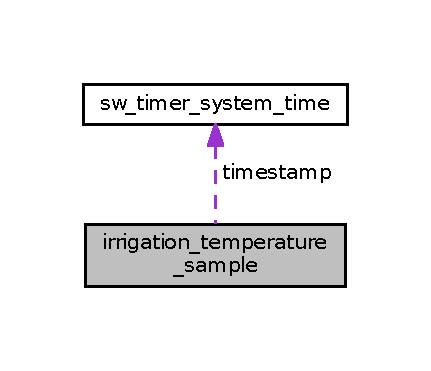
\includegraphics[width=207pt]{structirrigation__temperature__sample__coll__graph}
\end{center}
\end{figure}
\subsection*{Public Attributes}
\begin{DoxyCompactItemize}
\item 
struct \hyperlink{structsw__timer__system__time}{sw\+\_\+timer\+\_\+system\+\_\+time} \hyperlink{structirrigation__temperature__sample_aa10fbbf9f10f89fc9f246f42c26b0ad2}{timestamp}
\begin{DoxyCompactList}\small\item\em Time sample was taken. \end{DoxyCompactList}\item 
float \hyperlink{structirrigation__temperature__sample_ae72c8bc3c16a24366685eecbf9493a2e}{temperature}
\begin{DoxyCompactList}\small\item\em Temperature. \end{DoxyCompactList}\end{DoxyCompactItemize}


\subsection{Detailed Description}
This is a timestamped temperature sample. 

\subsection{Member Data Documentation}
\hypertarget{structirrigation__temperature__sample_ae72c8bc3c16a24366685eecbf9493a2e}{}\index{irrigation\+\_\+temperature\+\_\+sample@{irrigation\+\_\+temperature\+\_\+sample}!temperature@{temperature}}
\index{temperature@{temperature}!irrigation\+\_\+temperature\+\_\+sample@{irrigation\+\_\+temperature\+\_\+sample}}
\subsubsection[{temperature}]{\setlength{\rightskip}{0pt plus 5cm}float irrigation\+\_\+temperature\+\_\+sample\+::temperature}\label{structirrigation__temperature__sample_ae72c8bc3c16a24366685eecbf9493a2e}


Temperature. 

\hypertarget{structirrigation__temperature__sample_aa10fbbf9f10f89fc9f246f42c26b0ad2}{}\index{irrigation\+\_\+temperature\+\_\+sample@{irrigation\+\_\+temperature\+\_\+sample}!timestamp@{timestamp}}
\index{timestamp@{timestamp}!irrigation\+\_\+temperature\+\_\+sample@{irrigation\+\_\+temperature\+\_\+sample}}
\subsubsection[{timestamp}]{\setlength{\rightskip}{0pt plus 5cm}struct {\bf sw\+\_\+timer\+\_\+system\+\_\+time} irrigation\+\_\+temperature\+\_\+sample\+::timestamp}\label{structirrigation__temperature__sample_aa10fbbf9f10f89fc9f246f42c26b0ad2}


Time sample was taken. 



The documentation for this struct was generated from the following file\+:\begin{DoxyCompactItemize}
\item 
src/\hyperlink{irrigation_8h}{irrigation.\+h}\end{DoxyCompactItemize}

\hypertarget{classtest__lamp__2_1_1LED}{}\section{test\+\_\+lamp\+\_\+2.\+L\+E\+D Class Reference}
\label{classtest__lamp__2_1_1LED}\index{test\+\_\+lamp\+\_\+2.\+L\+E\+D@{test\+\_\+lamp\+\_\+2.\+L\+E\+D}}
\subsection*{Public Member Functions}
\begin{DoxyCompactItemize}
\item 
\hypertarget{classtest__lamp__2_1_1LED_a7ebc26ddc38b044ace63df4740e163e3}{}def {\bfseries \+\_\+\+\_\+init\+\_\+\+\_\+} (self)\label{classtest__lamp__2_1_1LED_a7ebc26ddc38b044ace63df4740e163e3}

\item 
\hypertarget{classtest__lamp__2_1_1LED_ab53d42f3dc9b52d1c0b91bbc0c01f6bc}{}def {\bfseries wait} (self, dt)\label{classtest__lamp__2_1_1LED_ab53d42f3dc9b52d1c0b91bbc0c01f6bc}

\item 
\hypertarget{classtest__lamp__2_1_1LED_a5bd051e74e3c9a340c055cf6f89cefed}{}def {\bfseries fade\+\_\+up} (self, dt)\label{classtest__lamp__2_1_1LED_a5bd051e74e3c9a340c055cf6f89cefed}

\item 
\hypertarget{classtest__lamp__2_1_1LED_a72a2b7823a6090e98c117791b9dfdb82}{}def {\bfseries fade\+\_\+down} (self, dt)\label{classtest__lamp__2_1_1LED_a72a2b7823a6090e98c117791b9dfdb82}

\item 
\hypertarget{classtest__lamp__2_1_1LED_a99111af75afcb2bcdc19a2b6030786ce}{}def {\bfseries think} (self, dt)\label{classtest__lamp__2_1_1LED_a99111af75afcb2bcdc19a2b6030786ce}

\item 
\hypertarget{classtest__lamp__2_1_1LED_aad3c3abd2f25347cb7ff2e59ec44bb22}{}def {\bfseries get\+\_\+struct} (self)\label{classtest__lamp__2_1_1LED_aad3c3abd2f25347cb7ff2e59ec44bb22}

\end{DoxyCompactItemize}
\subsection*{Public Attributes}
\begin{DoxyCompactItemize}
\item 
\hypertarget{classtest__lamp__2_1_1LED_a41c87b79c37a76cf50c4c0953289155e}{}{\bfseries i}\label{classtest__lamp__2_1_1LED_a41c87b79c37a76cf50c4c0953289155e}

\item 
\hypertarget{classtest__lamp__2_1_1LED_afb5082c08e48f00994c392fa217d2b09}{}{\bfseries hue}\label{classtest__lamp__2_1_1LED_afb5082c08e48f00994c392fa217d2b09}

\item 
\hypertarget{classtest__lamp__2_1_1LED_ac6f3c82e200c02b156c2784e226fa5dd}{}{\bfseries t}\label{classtest__lamp__2_1_1LED_ac6f3c82e200c02b156c2784e226fa5dd}

\item 
\hypertarget{classtest__lamp__2_1_1LED_a0e412e0c696e67f761031607303d5d06}{}{\bfseries wt}\label{classtest__lamp__2_1_1LED_a0e412e0c696e67f761031607303d5d06}

\item 
\hypertarget{classtest__lamp__2_1_1LED_a0db3ed45d4456ca7df9194ebebbb0ee5}{}{\bfseries mode}\label{classtest__lamp__2_1_1LED_a0db3ed45d4456ca7df9194ebebbb0ee5}

\end{DoxyCompactItemize}


The documentation for this class was generated from the following file\+:\begin{DoxyCompactItemize}
\item 
python\+\_\+scripts/test\+\_\+lamp\+\_\+2.\+py\end{DoxyCompactItemize}

\hypertarget{structsample__range}{}\section{sample\+\_\+range Struct Reference}
\label{structsample__range}\index{sample\+\_\+range@{sample\+\_\+range}}
\subsection*{Public Attributes}
\begin{DoxyCompactItemize}
\item 
\hypertarget{structsample__range_aec99a7b0ac9b940beae0e294c5a662c5}{}int {\bfseries min}\label{structsample__range_aec99a7b0ac9b940beae0e294c5a662c5}

\item 
\hypertarget{structsample__range_ac6d139bddb95ce94fea09eabcf9dfa8d}{}int {\bfseries max}\label{structsample__range_ac6d139bddb95ce94fea09eabcf9dfa8d}

\end{DoxyCompactItemize}


The documentation for this struct was generated from the following file\+:\begin{DoxyCompactItemize}
\item 
src/sampling.\+c\end{DoxyCompactItemize}

\hypertarget{structstate}{}\section{state Struct Reference}
\label{structstate}\index{state@{state}}
\subsection*{Public Attributes}
\begin{DoxyCompactItemize}
\item 
\hypertarget{structstate_a6524009fb107464c8bb47a14742c3f27}{}void($\ast$ {\bfseries enter} )(struct \hyperlink{structirrigation__controller}{irrigation\+\_\+controller} $\ast$)\label{structstate_a6524009fb107464c8bb47a14742c3f27}

\item 
\hypertarget{structstate_a64a1989f8b49bc262c04323be37d1d8c}{}void($\ast$ {\bfseries run} )(struct \hyperlink{structirrigation__controller}{irrigation\+\_\+controller} $\ast$)\label{structstate_a64a1989f8b49bc262c04323be37d1d8c}

\item 
\hypertarget{structstate_a4657a6bf0f9e2f16002217c54cb967cd}{}void($\ast$ {\bfseries exit} )(struct \hyperlink{structirrigation__controller}{irrigation\+\_\+controller} $\ast$)\label{structstate_a4657a6bf0f9e2f16002217c54cb967cd}

\item 
\hypertarget{structstate_a351d79011f95723018e1626646bb28c7}{}char $\ast$ {\bfseries name}\label{structstate_a351d79011f95723018e1626646bb28c7}

\end{DoxyCompactItemize}


The documentation for this struct was generated from the following file\+:\begin{DoxyCompactItemize}
\item 
src/\hyperlink{main_8c}{main.\+c}\end{DoxyCompactItemize}

\hypertarget{structsw__timer__system__time}{}\section{sw\+\_\+timer\+\_\+system\+\_\+time Struct Reference}
\label{structsw__timer__system__time}\index{sw\+\_\+timer\+\_\+system\+\_\+time@{sw\+\_\+timer\+\_\+system\+\_\+time}}
\subsection*{Public Attributes}
\begin{DoxyCompactItemize}
\item 
\hypertarget{structsw__timer__system__time_aa9f10bc219cafbf8c61f94fbb4138591}{}int {\bfseries epoch}\label{structsw__timer__system__time_aa9f10bc219cafbf8c61f94fbb4138591}

\item 
\hypertarget{structsw__timer__system__time_aafb47623ce45c3d1617e54d2025b679a}{}int {\bfseries ms}\label{structsw__timer__system__time_aafb47623ce45c3d1617e54d2025b679a}

\end{DoxyCompactItemize}


The documentation for this struct was generated from the following file\+:\begin{DoxyCompactItemize}
\item 
src/time.\+h\end{DoxyCompactItemize}

\hypertarget{structsystick}{}\section{systick Struct Reference}
\label{structsystick}\index{systick@{systick}}


Collaboration diagram for systick\+:\nopagebreak
\begin{figure}[H]
\begin{center}
\leavevmode
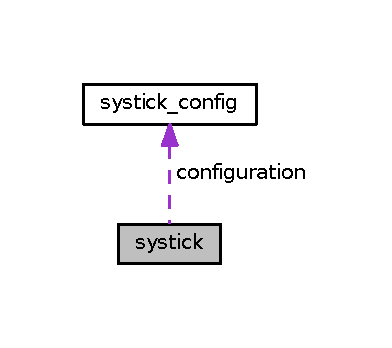
\includegraphics[width=188pt]{structsystick__coll__graph}
\end{center}
\end{figure}
\subsection*{Public Attributes}
\begin{DoxyCompactItemize}
\item 
\hypertarget{structsystick_a6e7d92e68eb2e575624d068b187ace33}{}struct \hyperlink{structsystick__config}{systick\+\_\+config} $\ast$ {\bfseries configuration}\label{structsystick_a6e7d92e68eb2e575624d068b187ace33}

\end{DoxyCompactItemize}


The documentation for this struct was generated from the following file\+:\begin{DoxyCompactItemize}
\item 
src/systick.\+h\end{DoxyCompactItemize}

\hypertarget{structsystick__config}{}\section{systick\+\_\+config Struct Reference}
\label{structsystick__config}\index{systick\+\_\+config@{systick\+\_\+config}}
\subsection*{Public Attributes}
\begin{DoxyCompactItemize}
\item 
\hypertarget{structsystick__config_a4234a833cb468e5ebe169bef99cb9235}{}uint32\+\_\+t {\bfseries frequency}\label{structsystick__config_a4234a833cb468e5ebe169bef99cb9235}

\item 
\hypertarget{structsystick__config_aa9f9da280ed0e328cdd0d0648a46aaad}{}bool {\bfseries auto\+\_\+start}\label{structsystick__config_aa9f9da280ed0e328cdd0d0648a46aaad}

\end{DoxyCompactItemize}


The documentation for this struct was generated from the following file\+:\begin{DoxyCompactItemize}
\item 
src/systick.\+h\end{DoxyCompactItemize}

\hypertarget{structtimer}{}\section{timer Struct Reference}
\label{structtimer}\index{timer@{timer}}


Collaboration diagram for timer\+:\nopagebreak
\begin{figure}[H]
\begin{center}
\leavevmode
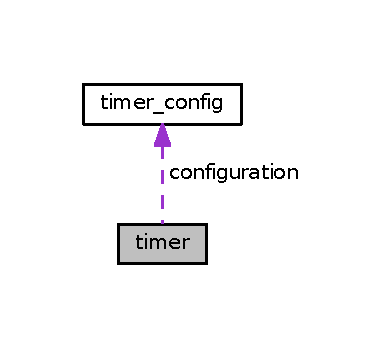
\includegraphics[width=184pt]{structtimer__coll__graph}
\end{center}
\end{figure}
\subsection*{Public Attributes}
\begin{DoxyCompactItemize}
\item 
\hypertarget{structtimer_a2bef740a83dc4af81d0dd6ef45dfbbfd}{}struct \hyperlink{structtimer__config}{timer\+\_\+config} $\ast$ {\bfseries configuration}\label{structtimer_a2bef740a83dc4af81d0dd6ef45dfbbfd}

\item 
\hypertarget{structtimer_a98106a5170cdde683d8bafc2a07ee7cd}{}enum \hyperlink{hw_8h_a3c02952100e7d051b77cdf060ca0ba9b}{hw\+\_\+init\+\_\+state} {\bfseries state}\label{structtimer_a98106a5170cdde683d8bafc2a07ee7cd}

\item 
\hypertarget{structtimer_af0cf0d2403679e91e1dd266ad60e421c}{}uint32\+\_\+t {\bfseries reload}\label{structtimer_af0cf0d2403679e91e1dd266ad60e421c}

\end{DoxyCompactItemize}


The documentation for this struct was generated from the following file\+:\begin{DoxyCompactItemize}
\item 
src/timer.\+h\end{DoxyCompactItemize}

\hypertarget{structtimer__ccr}{}\section{timer\+\_\+ccr Struct Reference}
\label{structtimer__ccr}\index{timer\+\_\+ccr@{timer\+\_\+ccr}}


Collaboration diagram for timer\+\_\+ccr\+:\nopagebreak
\begin{figure}[H]
\begin{center}
\leavevmode
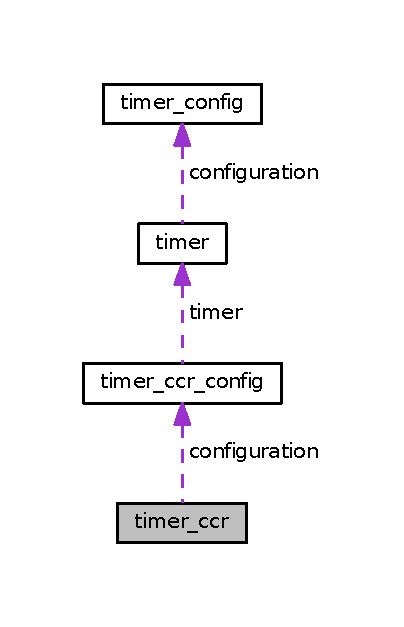
\includegraphics[width=194pt]{structtimer__ccr__coll__graph}
\end{center}
\end{figure}
\subsection*{Public Attributes}
\begin{DoxyCompactItemize}
\item 
\hypertarget{structtimer__ccr_ae53385b34f3535fa8cc732edc5fccc28}{}struct \hyperlink{structtimer__ccr__config}{timer\+\_\+ccr\+\_\+config} $\ast$ {\bfseries configuration}\label{structtimer__ccr_ae53385b34f3535fa8cc732edc5fccc28}

\item 
\hypertarget{structtimer__ccr_addba2954b9a68f87a1e716a65095c6a9}{}enum \hyperlink{hw_8h_a3c02952100e7d051b77cdf060ca0ba9b}{hw\+\_\+init\+\_\+state} {\bfseries state}\label{structtimer__ccr_addba2954b9a68f87a1e716a65095c6a9}

\end{DoxyCompactItemize}


The documentation for this struct was generated from the following file\+:\begin{DoxyCompactItemize}
\item 
src/timer.\+h\end{DoxyCompactItemize}

\hypertarget{structtimer__ccr__config}{}\section{timer\+\_\+ccr\+\_\+config Struct Reference}
\label{structtimer__ccr__config}\index{timer\+\_\+ccr\+\_\+config@{timer\+\_\+ccr\+\_\+config}}


Collaboration diagram for timer\+\_\+ccr\+\_\+config\+:\nopagebreak
\begin{figure}[H]
\begin{center}
\leavevmode
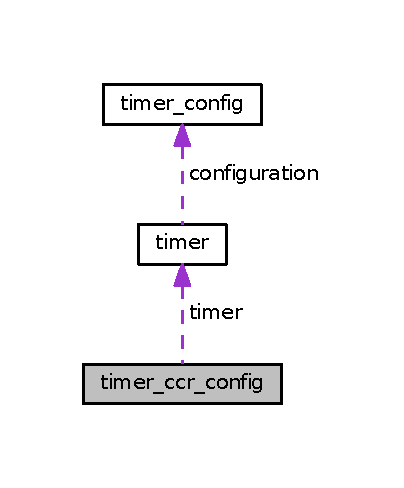
\includegraphics[width=194pt]{structtimer__ccr__config__coll__graph}
\end{center}
\end{figure}
\subsection*{Public Attributes}
\begin{DoxyCompactItemize}
\item 
\hypertarget{structtimer__ccr__config_af228e92c83395be0dff9f27e6ba7711a}{}struct \hyperlink{structtimer}{timer} $\ast$ {\bfseries timer}\label{structtimer__ccr__config_af228e92c83395be0dff9f27e6ba7711a}

\item 
\hypertarget{structtimer__ccr__config_ae497ec8b539565c6fe34b2849989336a}{}enum tim\+\_\+oc\+\_\+id {\bfseries channel}\label{structtimer__ccr__config_ae497ec8b539565c6fe34b2849989336a}

\item 
\hypertarget{structtimer__ccr__config_a2fb041bdd23dfe84fc7aebb6c51fc149}{}uint32\+\_\+t {\bfseries start\+\_\+ccr}\label{structtimer__ccr__config_a2fb041bdd23dfe84fc7aebb6c51fc149}

\item 
\hypertarget{structtimer__ccr__config_a3876bca410f69a23790a94f8eb9d73f8}{}volatile uint32\+\_\+t $\ast$ {\bfseries reg}\label{structtimer__ccr__config_a3876bca410f69a23790a94f8eb9d73f8}

\item 
\hypertarget{structtimer__ccr__config_a191d86d5e9bc07494477cb7cb39f3a6c}{}uint32\+\_\+t {\bfseries dma\+\_\+channel}\label{structtimer__ccr__config_a191d86d5e9bc07494477cb7cb39f3a6c}

\item 
\hypertarget{structtimer__ccr__config_aa53eb7bbe594fdffff8537f281167e2d}{}uint32\+\_\+t {\bfseries dma\+\_\+enable\+\_\+flag}\label{structtimer__ccr__config_aa53eb7bbe594fdffff8537f281167e2d}

\end{DoxyCompactItemize}


The documentation for this struct was generated from the following file\+:\begin{DoxyCompactItemize}
\item 
src/timer.\+h\end{DoxyCompactItemize}

\hypertarget{structtimer__config}{}\section{timer\+\_\+config Struct Reference}
\label{structtimer__config}\index{timer\+\_\+config@{timer\+\_\+config}}
\subsection*{Public Attributes}
\begin{DoxyCompactItemize}
\item 
\hypertarget{structtimer__config_afed1f1ae48fa09893427efa6b8338b65}{}uint32\+\_\+t {\bfseries timer}\label{structtimer__config_afed1f1ae48fa09893427efa6b8338b65}

\item 
\hypertarget{structtimer__config_a1591c4486ebf07c8ac73e69acbbbbc3a}{}uint32\+\_\+t {\bfseries rcc}\label{structtimer__config_a1591c4486ebf07c8ac73e69acbbbbc3a}

\item 
\hypertarget{structtimer__config_a492b92e61d66e088574be5cc00d10710}{}uint32\+\_\+t {\bfseries dma\+\_\+rcc}\label{structtimer__config_a492b92e61d66e088574be5cc00d10710}

\item 
\hypertarget{structtimer__config_af0af259e1730fdfeebd34344f5a5fa1b}{}uint32\+\_\+t {\bfseries auto\+\_\+reload}\label{structtimer__config_af0af259e1730fdfeebd34344f5a5fa1b}

\end{DoxyCompactItemize}


The documentation for this struct was generated from the following file\+:\begin{DoxyCompactItemize}
\item 
src/timer.\+h\end{DoxyCompactItemize}

\hypertarget{structtm}{}\section{tm Struct Reference}
\label{structtm}\index{tm@{tm}}
\subsection*{Public Attributes}
\begin{DoxyCompactItemize}
\item 
\hypertarget{structtm_a4d098a9a5c03a00b2ee61e10851de81e}{}int {\bfseries tm\+\_\+sec}\label{structtm_a4d098a9a5c03a00b2ee61e10851de81e}

\item 
\hypertarget{structtm_af414eb7c86cc3099595211eee4d4211b}{}int {\bfseries tm\+\_\+min}\label{structtm_af414eb7c86cc3099595211eee4d4211b}

\item 
\hypertarget{structtm_a3e7ca4e37f1abcaf56b8a916c38eb9fe}{}int {\bfseries tm\+\_\+hour}\label{structtm_a3e7ca4e37f1abcaf56b8a916c38eb9fe}

\item 
\hypertarget{structtm_ab8d8904bad43b0c8b96e61941c5b5310}{}int {\bfseries tm\+\_\+mday}\label{structtm_ab8d8904bad43b0c8b96e61941c5b5310}

\item 
\hypertarget{structtm_a112ac36fa2f593777138a417cf031e17}{}int {\bfseries tm\+\_\+mon}\label{structtm_a112ac36fa2f593777138a417cf031e17}

\item 
\hypertarget{structtm_a33adf78fd6476b2120ce3b9c4a852053}{}int {\bfseries tm\+\_\+year}\label{structtm_a33adf78fd6476b2120ce3b9c4a852053}

\item 
\hypertarget{structtm_afe81a8c46f1c693c43f259b288859f4f}{}int {\bfseries tm\+\_\+wday}\label{structtm_afe81a8c46f1c693c43f259b288859f4f}

\item 
\hypertarget{structtm_a93a0ba77cc23796df84405dcbcc57eb1}{}int {\bfseries tm\+\_\+yday}\label{structtm_a93a0ba77cc23796df84405dcbcc57eb1}

\item 
\hypertarget{structtm_a5645ca0580c8ab2c24f6c2965d9c9f9c}{}int {\bfseries tm\+\_\+isdst}\label{structtm_a5645ca0580c8ab2c24f6c2965d9c9f9c}

\end{DoxyCompactItemize}


The documentation for this struct was generated from the following file\+:\begin{DoxyCompactItemize}
\item 
src/time.\+h\end{DoxyCompactItemize}

\hypertarget{structusart}{}\section{usart Struct Reference}
\label{structusart}\index{usart@{usart}}


Collaboration diagram for usart\+:\nopagebreak
\begin{figure}[H]
\begin{center}
\leavevmode
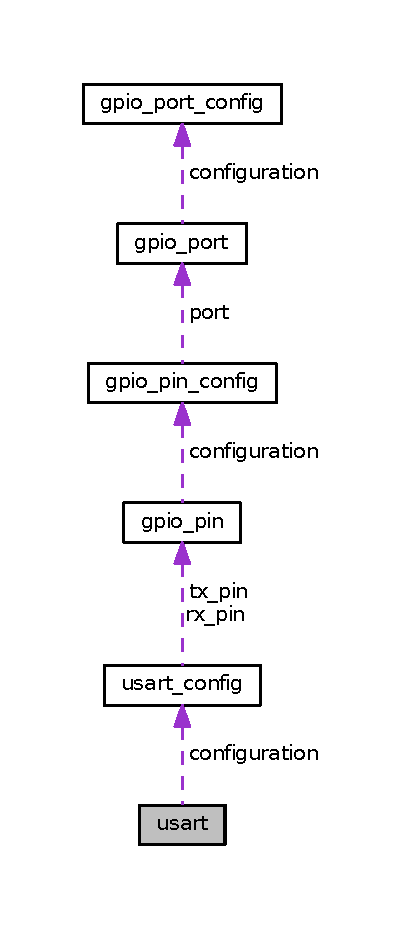
\includegraphics[width=194pt]{structusart__coll__graph}
\end{center}
\end{figure}
\subsection*{Public Attributes}
\begin{DoxyCompactItemize}
\item 
\hypertarget{structusart_a42f49f07a75c1ec44a8a1e04e08a760c}{}struct \hyperlink{structusart__config}{usart\+\_\+config} $\ast$ {\bfseries configuration}\label{structusart_a42f49f07a75c1ec44a8a1e04e08a760c}

\end{DoxyCompactItemize}


The documentation for this struct was generated from the following file\+:\begin{DoxyCompactItemize}
\item 
src/uart.\+h\end{DoxyCompactItemize}

\hypertarget{structusart__config}{}\section{usart\+\_\+config Struct Reference}
\label{structusart__config}\index{usart\+\_\+config@{usart\+\_\+config}}


Collaboration diagram for usart\+\_\+config\+:\nopagebreak
\begin{figure}[H]
\begin{center}
\leavevmode
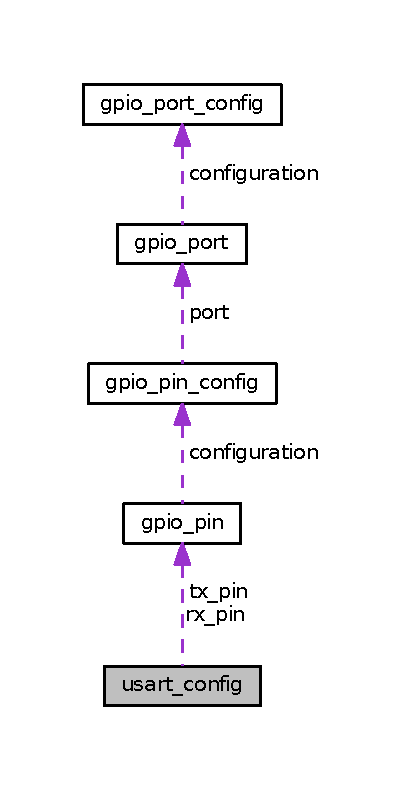
\includegraphics[width=194pt]{structusart__config__coll__graph}
\end{center}
\end{figure}
\subsection*{Public Attributes}
\begin{DoxyCompactItemize}
\item 
\hypertarget{structusart__config_afb0c0a9281bba234d1b7282fd5661826}{}struct \hyperlink{structgpio__pin}{gpio\+\_\+pin} $\ast$ {\bfseries rx\+\_\+pin}\label{structusart__config_afb0c0a9281bba234d1b7282fd5661826}

\item 
\hypertarget{structusart__config_acda049cae41a8261b02b52ef76830941}{}struct \hyperlink{structgpio__pin}{gpio\+\_\+pin} $\ast$ {\bfseries tx\+\_\+pin}\label{structusart__config_acda049cae41a8261b02b52ef76830941}

\item 
\hypertarget{structusart__config_a7057d1e4e59d4cb6f002cace870fa34b}{}uint32\+\_\+t {\bfseries usart}\label{structusart__config_a7057d1e4e59d4cb6f002cace870fa34b}

\item 
\hypertarget{structusart__config_a5362ef6b4daf5a9e2722c9c4e167e9ed}{}uint32\+\_\+t {\bfseries rcc}\label{structusart__config_a5362ef6b4daf5a9e2722c9c4e167e9ed}

\item 
\hypertarget{structusart__config_acacbd7ecb3d46f576ff1361ae40019fd}{}uint32\+\_\+t {\bfseries baudrate}\label{structusart__config_acacbd7ecb3d46f576ff1361ae40019fd}

\item 
\hypertarget{structusart__config_a688b390f173cc710c95227d84a8f0771}{}uint32\+\_\+t {\bfseries databits}\label{structusart__config_a688b390f173cc710c95227d84a8f0771}

\item 
\hypertarget{structusart__config_a69189444320b793047313d2e80c9df6b}{}uint32\+\_\+t {\bfseries parity}\label{structusart__config_a69189444320b793047313d2e80c9df6b}

\item 
\hypertarget{structusart__config_a5d944fbbe5a88c9a2f2d60df6a092f69}{}uint32\+\_\+t {\bfseries stopbits}\label{structusart__config_a5d944fbbe5a88c9a2f2d60df6a092f69}

\item 
\hypertarget{structusart__config_afaf14d61e3be8a4d3208a1acb68967d4}{}uint32\+\_\+t {\bfseries mode}\label{structusart__config_afaf14d61e3be8a4d3208a1acb68967d4}

\item 
\hypertarget{structusart__config_aef2d53d38b3b8b974a5e3355061f9ec8}{}uint32\+\_\+t {\bfseries flowcontrol}\label{structusart__config_aef2d53d38b3b8b974a5e3355061f9ec8}

\end{DoxyCompactItemize}


The documentation for this struct was generated from the following file\+:\begin{DoxyCompactItemize}
\item 
src/uart.\+h\end{DoxyCompactItemize}

\hypertarget{classv3_1_1vec3}{}\section{v3.\+vec3 Class Reference}
\label{classv3_1_1vec3}\index{v3.\+vec3@{v3.\+vec3}}
\subsection*{Public Member Functions}
\begin{DoxyCompactItemize}
\item 
\hypertarget{classv3_1_1vec3_a6b71dd959cfe38cdfc1e97fb170e1e64}{}def {\bfseries \+\_\+\+\_\+init\+\_\+\+\_\+}\label{classv3_1_1vec3_a6b71dd959cfe38cdfc1e97fb170e1e64}

\item 
\hypertarget{classv3_1_1vec3_a9d57a93db63fa0541a4701e7a23069ef}{}def {\bfseries \+\_\+\+\_\+abs\+\_\+\+\_\+} (self)\label{classv3_1_1vec3_a9d57a93db63fa0541a4701e7a23069ef}

\item 
\hypertarget{classv3_1_1vec3_a74328d6c6bc5158e0eb047c71360147a}{}def {\bfseries \+\_\+\+\_\+iter\+\_\+\+\_\+} (self)\label{classv3_1_1vec3_a74328d6c6bc5158e0eb047c71360147a}

\item 
\hypertarget{classv3_1_1vec3_a8fd8168bd72eaa605539a2d6a46ab8d8}{}def {\bfseries get\+\_\+normalized} (self)\label{classv3_1_1vec3_a8fd8168bd72eaa605539a2d6a46ab8d8}

\item 
\hypertarget{classv3_1_1vec3_a9c631bf20da30777f24ec3012fc1c54e}{}def {\bfseries \+\_\+\+\_\+sub\+\_\+\+\_\+} (self, other)\label{classv3_1_1vec3_a9c631bf20da30777f24ec3012fc1c54e}

\item 
\hypertarget{classv3_1_1vec3_a747b885a97da891d8da838dd4ee121fe}{}def {\bfseries \+\_\+\+\_\+add\+\_\+\+\_\+} (self, other)\label{classv3_1_1vec3_a747b885a97da891d8da838dd4ee121fe}

\item 
\hypertarget{classv3_1_1vec3_a32ef2c056e8b4da011bf45ad0bad1293}{}def {\bfseries \+\_\+\+\_\+div\+\_\+\+\_\+} (self, other)\label{classv3_1_1vec3_a32ef2c056e8b4da011bf45ad0bad1293}

\item 
\hypertarget{classv3_1_1vec3_ae3c44b93d824783efdf4fbe6a86ef268}{}def {\bfseries \+\_\+\+\_\+mul\+\_\+\+\_\+} (self, other)\label{classv3_1_1vec3_ae3c44b93d824783efdf4fbe6a86ef268}

\item 
\hypertarget{classv3_1_1vec3_a9d7d44a7c1606c868c9dbcaf33ce5ffa}{}def {\bfseries \+\_\+\+\_\+repr\+\_\+\+\_\+} (self)\label{classv3_1_1vec3_a9d7d44a7c1606c868c9dbcaf33ce5ffa}

\item 
\hypertarget{classv3_1_1vec3_ac3bab8cc971bb073dcef29c4b93cb8a3}{}def {\bfseries \+\_\+\+\_\+setitem\+\_\+\+\_\+} (self, index, value)\label{classv3_1_1vec3_ac3bab8cc971bb073dcef29c4b93cb8a3}

\end{DoxyCompactItemize}
\subsection*{Public Attributes}
\begin{DoxyCompactItemize}
\item 
\hypertarget{classv3_1_1vec3_a1df675426a46bf6d78ae23844c327061}{}{\bfseries z}\label{classv3_1_1vec3_a1df675426a46bf6d78ae23844c327061}

\item 
\hypertarget{classv3_1_1vec3_a8140d9ed95b6487006ca20342bc96fc0}{}{\bfseries x}\label{classv3_1_1vec3_a8140d9ed95b6487006ca20342bc96fc0}

\item 
\hypertarget{classv3_1_1vec3_a5971d16eae14a2e3e3fb451134a7aff7}{}{\bfseries y}\label{classv3_1_1vec3_a5971d16eae14a2e3e3fb451134a7aff7}

\end{DoxyCompactItemize}


The documentation for this class was generated from the following file\+:\begin{DoxyCompactItemize}
\item 
python\+\_\+scripts/v3.\+py\end{DoxyCompactItemize}

\hypertarget{structws2812}{}\section{ws2812 Struct Reference}
\label{structws2812}\index{ws2812@{ws2812}}


Collaboration diagram for ws2812\+:\nopagebreak
\begin{figure}[H]
\begin{center}
\leavevmode
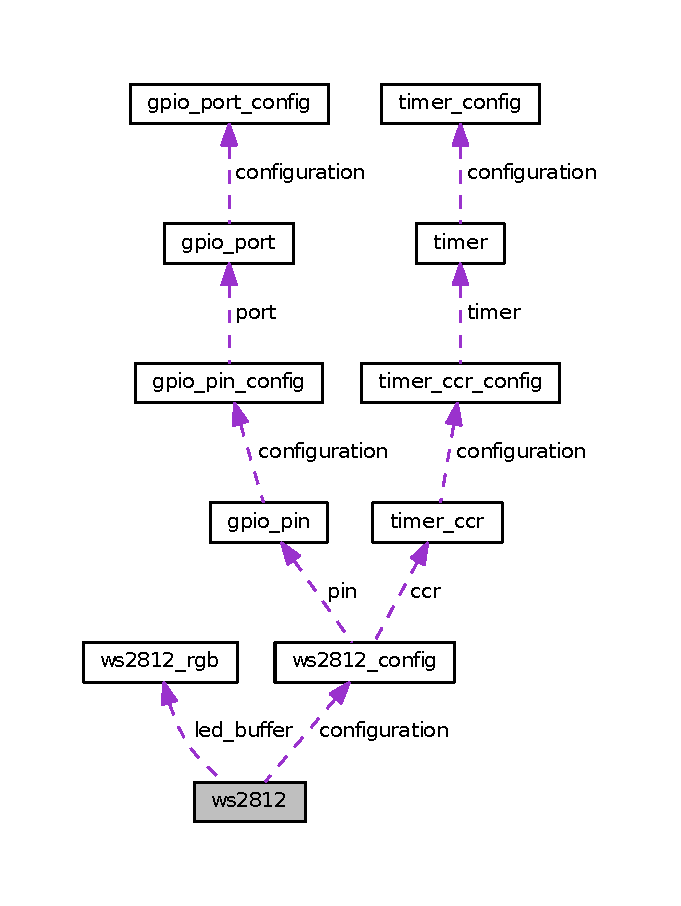
\includegraphics[width=327pt]{structws2812__coll__graph}
\end{center}
\end{figure}
\subsection*{Public Attributes}
\begin{DoxyCompactItemize}
\item 
\hypertarget{structws2812_a4b69cc515557cd305ebfd3372fc09f81}{}struct \hyperlink{structws2812__config}{ws2812\+\_\+config} $\ast$ {\bfseries configuration}\label{structws2812_a4b69cc515557cd305ebfd3372fc09f81}

\item 
\hypertarget{structws2812_a9d672a2d9ea381c7fcd940ba4ebdebe2}{}struct \hyperlink{structws2812__rgb}{ws2812\+\_\+rgb} $\ast$ {\bfseries led\+\_\+buffer}\label{structws2812_a9d672a2d9ea381c7fcd940ba4ebdebe2}

\item 
\hypertarget{structws2812_a61297f46cd5f505ca589214d93bcbc13}{}uint8\+\_\+t $\ast$ {\bfseries pwm\+\_\+buffer}\label{structws2812_a61297f46cd5f505ca589214d93bcbc13}

\item 
\hypertarget{structws2812_a396b295c928e75adc5688c49c832e631}{}enum \hyperlink{hw_8h_a3c02952100e7d051b77cdf060ca0ba9b}{hw\+\_\+init\+\_\+state} {\bfseries state}\label{structws2812_a396b295c928e75adc5688c49c832e631}

\item 
\hypertarget{structws2812_aaed6db83ce4a0e8e58b73650f2b4638e}{}int {\bfseries led\+\_\+count}\label{structws2812_aaed6db83ce4a0e8e58b73650f2b4638e}

\end{DoxyCompactItemize}


The documentation for this struct was generated from the following file\+:\begin{DoxyCompactItemize}
\item 
src/ws2812.\+h\end{DoxyCompactItemize}

\hypertarget{structws2812__config}{}\section{ws2812\+\_\+config Struct Reference}
\label{structws2812__config}\index{ws2812\+\_\+config@{ws2812\+\_\+config}}


Collaboration diagram for ws2812\+\_\+config\+:\nopagebreak
\begin{figure}[H]
\begin{center}
\leavevmode
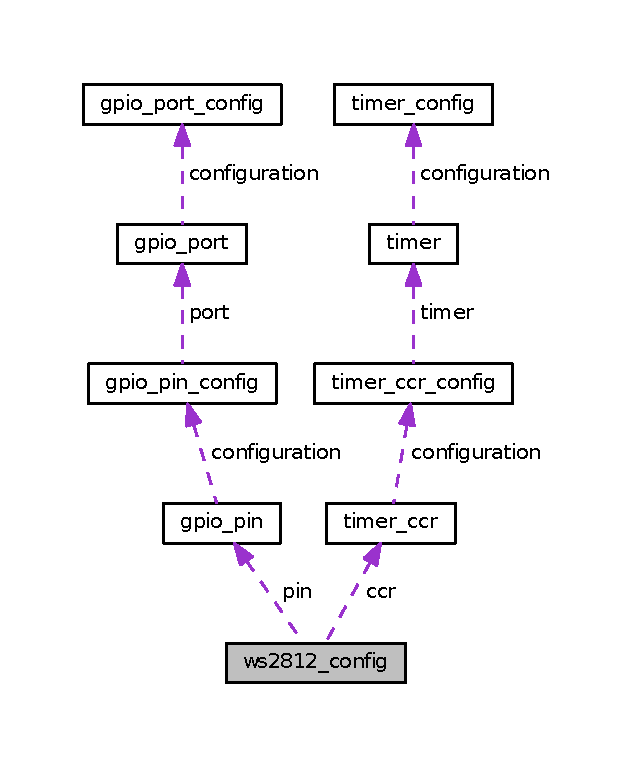
\includegraphics[width=305pt]{structws2812__config__coll__graph}
\end{center}
\end{figure}
\subsection*{Public Attributes}
\begin{DoxyCompactItemize}
\item 
\hypertarget{structws2812__config_a0c4b50ce11c055c0457af653c4951ee9}{}struct \hyperlink{structtimer__ccr}{timer\+\_\+ccr} $\ast$ {\bfseries ccr}\label{structws2812__config_a0c4b50ce11c055c0457af653c4951ee9}

\item 
\hypertarget{structws2812__config_a665ce3190145f97af1d234f9de5defc1}{}struct \hyperlink{structgpio__pin}{gpio\+\_\+pin} $\ast$ {\bfseries pin}\label{structws2812__config_a665ce3190145f97af1d234f9de5defc1}

\item 
\hypertarget{structws2812__config_a15634a419d7f20275ec1e6ba1215920b}{}uint32\+\_\+t {\bfseries frequency}\label{structws2812__config_a15634a419d7f20275ec1e6ba1215920b}

\item 
\hypertarget{structws2812__config_a22370b6dc4cdf5c6e25c4c155a275046}{}uint32\+\_\+t {\bfseries bit0}\label{structws2812__config_a22370b6dc4cdf5c6e25c4c155a275046}

\item 
\hypertarget{structws2812__config_a410b277b06bbb4ff2f8fd8c6fb5bc994}{}uint32\+\_\+t {\bfseries bit1}\label{structws2812__config_a410b277b06bbb4ff2f8fd8c6fb5bc994}

\end{DoxyCompactItemize}


The documentation for this struct was generated from the following file\+:\begin{DoxyCompactItemize}
\item 
src/ws2812.\+h\end{DoxyCompactItemize}

\hypertarget{structws2812__rgb}{}\section{ws2812\+\_\+rgb Struct Reference}
\label{structws2812__rgb}\index{ws2812\+\_\+rgb@{ws2812\+\_\+rgb}}
\subsection*{Public Attributes}
\begin{DoxyCompactItemize}
\item 
\hypertarget{structws2812__rgb_accf7188c624788256477c2e4ee54515b}{}uint8\+\_\+t {\bfseries r}\label{structws2812__rgb_accf7188c624788256477c2e4ee54515b}

\item 
\hypertarget{structws2812__rgb_aaf5b0f4db796641e1cd16bd4f70fc7ac}{}uint8\+\_\+t {\bfseries g}\label{structws2812__rgb_aaf5b0f4db796641e1cd16bd4f70fc7ac}

\item 
\hypertarget{structws2812__rgb_ae6d6d19362a79c36178203b3123d2e7e}{}uint8\+\_\+t {\bfseries b}\label{structws2812__rgb_ae6d6d19362a79c36178203b3123d2e7e}

\end{DoxyCompactItemize}


The documentation for this struct was generated from the following file\+:\begin{DoxyCompactItemize}
\item 
src/ws2812.\+h\end{DoxyCompactItemize}

\chapter{File Documentation}
\hypertarget{hw_8h}{}\section{src/hw.h File Reference}
\label{hw_8h}\index{src/hw.\+h@{src/hw.\+h}}


Hardware abstraction layer include file.  


This graph shows which files directly or indirectly include this file\+:
\nopagebreak
\begin{figure}[H]
\begin{center}
\leavevmode
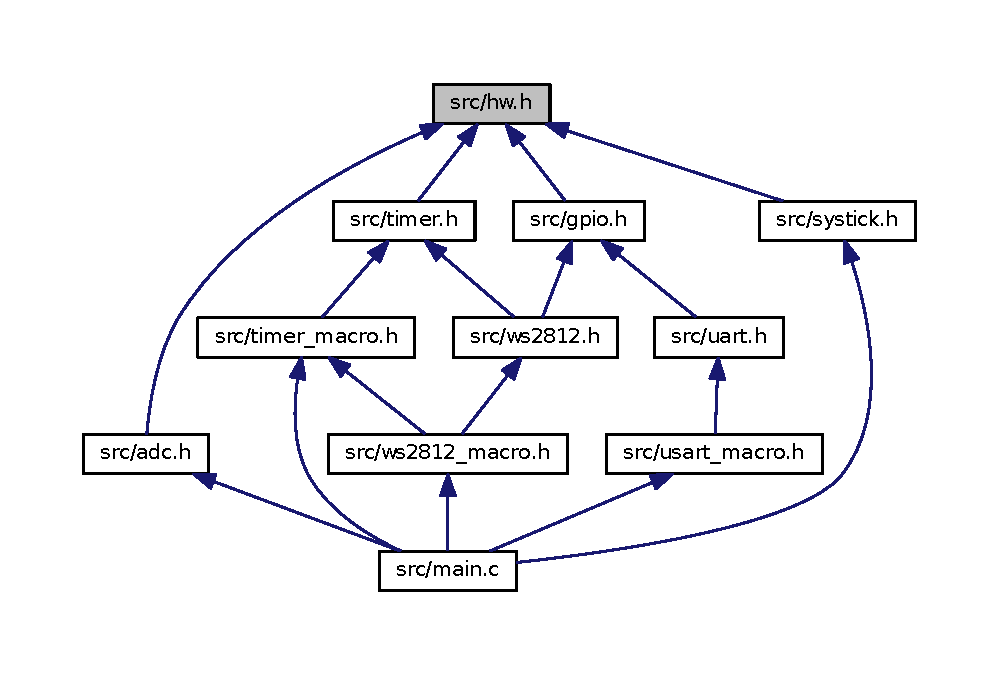
\includegraphics[width=350pt]{hw_8h__dep__incl}
\end{center}
\end{figure}
\subsection*{Macros}
\begin{DoxyCompactItemize}
\item 
\hypertarget{hw_8h_a40deaf267e014e0489a474b8eb6f7378}{}\#define {\bfseries D\+E\+F\+A\+U\+L\+T}(value,  default)~value = value ? value \+: default\label{hw_8h_a40deaf267e014e0489a474b8eb6f7378}

\item 
\hypertarget{hw_8h_a2c9e85d22a9ba37ea589b1747af46307}{}\#define {\bfseries V\+R\+E\+F}~3.\+295\label{hw_8h_a2c9e85d22a9ba37ea589b1747af46307}

\item 
\hypertarget{hw_8h_a918f64eb53db8e8dc694f36a87646476}{}\#define {\bfseries R1}~100000.\+0\label{hw_8h_a918f64eb53db8e8dc694f36a87646476}

\item 
\hypertarget{hw_8h_aa6d350d439222376ecc6da4bb50403c2}{}\#define {\bfseries N\+T\+C\+\_\+\+R}~150000\label{hw_8h_aa6d350d439222376ecc6da4bb50403c2}

\item 
\hypertarget{hw_8h_a18525dcee03997cc094fdf30c82fbf1c}{}\#define {\bfseries N\+T\+C\+\_\+\+A1}~3.\+354016\+E-\/03\label{hw_8h_a18525dcee03997cc094fdf30c82fbf1c}

\item 
\hypertarget{hw_8h_a203d2ab7a8a9a70d5455888b923d341b}{}\#define {\bfseries N\+T\+C\+\_\+\+B1}~2.\+367720\+E-\/04\label{hw_8h_a203d2ab7a8a9a70d5455888b923d341b}

\item 
\hypertarget{hw_8h_ab9a7131a2fb1b8f70f428e5198ada9c1}{}\#define {\bfseries N\+T\+C\+\_\+\+C1}~3.\+585140\+E-\/06\label{hw_8h_ab9a7131a2fb1b8f70f428e5198ada9c1}

\item 
\hypertarget{hw_8h_aecc61ee6e79b14087f05cd59f8252898}{}\#define {\bfseries N\+T\+C\+\_\+\+D1}~1.\+255349\+E-\/07\label{hw_8h_aecc61ee6e79b14087f05cd59f8252898}

\item 
\hypertarget{hw_8h_a16b6412d50d047f1699f6882b7166d24}{}\#define {\bfseries T0\+\_\+\+K}~273.\+15\label{hw_8h_a16b6412d50d047f1699f6882b7166d24}

\item 
\hypertarget{hw_8h_aacaca0988244bd3a888ca5befa89f44b}{}\#define {\bfseries P\+W\+M\+\_\+\+P\+E\+R\+I\+O\+D}~4096\label{hw_8h_aacaca0988244bd3a888ca5befa89f44b}

\item 
\hypertarget{hw_8h_a0565d8b2c16056c3a4d9f916a7fe2ef3}{}\#define {\bfseries P\+W\+M\+\_\+\+T\+O\+P}~(P\+W\+M\+\_\+\+P\+E\+R\+I\+O\+D -\/ 1)\label{hw_8h_a0565d8b2c16056c3a4d9f916a7fe2ef3}

\item 
\hypertarget{hw_8h_aad6d4d2ba34b16b7fa27f303d506ef71}{}\#define {\bfseries \+\_\+\+H\+W\+\_\+\+H\+\_\+}\label{hw_8h_aad6d4d2ba34b16b7fa27f303d506ef71}

\end{DoxyCompactItemize}
\subsection*{Enumerations}
\begin{DoxyCompactItemize}
\item 
enum \hyperlink{hw_8h_a3c02952100e7d051b77cdf060ca0ba9b}{hw\+\_\+init\+\_\+state} \{ \\*
\hyperlink{hw_8h_a3c02952100e7d051b77cdf060ca0ba9ba6b96182ed0808ff30887f91b24d86849}{H\+W\+\_\+\+I\+N\+I\+T\+\_\+\+U\+N\+I\+N\+I\+T\+I\+A\+L\+I\+Z\+E\+D}, 
\hyperlink{hw_8h_a3c02952100e7d051b77cdf060ca0ba9baca0b4dbf0e3911b3edde56d700f76ecf}{H\+W\+\_\+\+I\+N\+I\+T\+\_\+\+R\+C\+C}, 
\hyperlink{hw_8h_a3c02952100e7d051b77cdf060ca0ba9ba4e9b2d4b7e946d95c2e41f3de17035a0}{H\+W\+\_\+\+I\+N\+I\+T\+\_\+\+G\+P\+I\+O}, 
\hyperlink{hw_8h_a3c02952100e7d051b77cdf060ca0ba9ba45012c00c17031e71a4f60ada04df07d}{H\+W\+\_\+\+I\+N\+I\+T\+\_\+\+P\+R\+E\+\_\+\+N\+V\+I\+C}, 
\\*
\hyperlink{hw_8h_a3c02952100e7d051b77cdf060ca0ba9ba3f137ea5dd6b2ac372bb6d175434b3fa}{H\+W\+\_\+\+I\+N\+I\+T\+\_\+\+N\+V\+I\+C}, 
\hyperlink{hw_8h_a3c02952100e7d051b77cdf060ca0ba9bacf9b04dc351d9fc47482fcd5229eb201}{H\+W\+\_\+\+I\+N\+I\+T\+\_\+\+P\+O\+S\+T\+\_\+\+I\+N\+I\+T}, 
{\bfseries H\+W\+\_\+\+I\+N\+I\+T\+\_\+\+I\+N\+I\+T\+I\+A\+L\+I\+Z\+E\+D}
 \}
\begin{DoxyCompactList}\small\item\em This is the state of the hardware abstraction layer. \end{DoxyCompactList}\end{DoxyCompactItemize}
\subsection*{Functions}
\begin{DoxyCompactItemize}
\item 
\hypertarget{hw_8h_acf938165e604a675fe09218a1b3cfb5f}{}void {\bfseries hw\+\_\+init} ()\label{hw_8h_acf938165e604a675fe09218a1b3cfb5f}

\item 
void \hyperlink{hw_8h_aabae29cd362c0001a2b417c9206cb330}{hw\+\_\+init\+\_\+state} (enum \hyperlink{hw_8h_a3c02952100e7d051b77cdf060ca0ba9b}{hw\+\_\+init\+\_\+state} \hyperlink{structstate}{state})
\begin{DoxyCompactList}\small\item\em This function prototype calls all perhipherals with the state as argument. \end{DoxyCompactList}\end{DoxyCompactItemize}


\subsection{Detailed Description}
Hardware abstraction layer include file. 

\begin{DoxyRefDesc}{Todo}
\item[\hyperlink{todo__todo000001}{Todo}]There is some stuff not belonging to this file in here, it should be moved\end{DoxyRefDesc}


The hardware abstraction layer should be completely generic except that it initializes the system in a predefined order 

\subsection{Enumeration Type Documentation}
\hypertarget{hw_8h_a3c02952100e7d051b77cdf060ca0ba9b}{}\index{hw.\+h@{hw.\+h}!hw\+\_\+init\+\_\+state@{hw\+\_\+init\+\_\+state}}
\index{hw\+\_\+init\+\_\+state@{hw\+\_\+init\+\_\+state}!hw.\+h@{hw.\+h}}
\subsubsection[{hw\+\_\+init\+\_\+state}]{\setlength{\rightskip}{0pt plus 5cm}enum {\bf hw\+\_\+init\+\_\+state}}\label{hw_8h_a3c02952100e7d051b77cdf060ca0ba9b}


This is the state of the hardware abstraction layer. 

\begin{Desc}
\item[Enumerator]\par
\begin{description}
\index{H\+W\+\_\+\+I\+N\+I\+T\+\_\+\+U\+N\+I\+N\+I\+T\+I\+A\+L\+I\+Z\+E\+D@{H\+W\+\_\+\+I\+N\+I\+T\+\_\+\+U\+N\+I\+N\+I\+T\+I\+A\+L\+I\+Z\+E\+D}!hw.\+h@{hw.\+h}}\index{hw.\+h@{hw.\+h}!H\+W\+\_\+\+I\+N\+I\+T\+\_\+\+U\+N\+I\+N\+I\+T\+I\+A\+L\+I\+Z\+E\+D@{H\+W\+\_\+\+I\+N\+I\+T\+\_\+\+U\+N\+I\+N\+I\+T\+I\+A\+L\+I\+Z\+E\+D}}\item[{\em 
\hypertarget{hw_8h_a3c02952100e7d051b77cdf060ca0ba9ba6b96182ed0808ff30887f91b24d86849}{}H\+W\+\_\+\+I\+N\+I\+T\+\_\+\+U\+N\+I\+N\+I\+T\+I\+A\+L\+I\+Z\+E\+D\label{hw_8h_a3c02952100e7d051b77cdf060ca0ba9ba6b96182ed0808ff30887f91b24d86849}
}]Hardware is not initialized. \index{H\+W\+\_\+\+I\+N\+I\+T\+\_\+\+R\+C\+C@{H\+W\+\_\+\+I\+N\+I\+T\+\_\+\+R\+C\+C}!hw.\+h@{hw.\+h}}\index{hw.\+h@{hw.\+h}!H\+W\+\_\+\+I\+N\+I\+T\+\_\+\+R\+C\+C@{H\+W\+\_\+\+I\+N\+I\+T\+\_\+\+R\+C\+C}}\item[{\em 
\hypertarget{hw_8h_a3c02952100e7d051b77cdf060ca0ba9baca0b4dbf0e3911b3edde56d700f76ecf}{}H\+W\+\_\+\+I\+N\+I\+T\+\_\+\+R\+C\+C\label{hw_8h_a3c02952100e7d051b77cdf060ca0ba9baca0b4dbf0e3911b3edde56d700f76ecf}
}]This is the first state entered and here hardware drivers may initialize any clocks needed. \index{H\+W\+\_\+\+I\+N\+I\+T\+\_\+\+G\+P\+I\+O@{H\+W\+\_\+\+I\+N\+I\+T\+\_\+\+G\+P\+I\+O}!hw.\+h@{hw.\+h}}\index{hw.\+h@{hw.\+h}!H\+W\+\_\+\+I\+N\+I\+T\+\_\+\+G\+P\+I\+O@{H\+W\+\_\+\+I\+N\+I\+T\+\_\+\+G\+P\+I\+O}}\item[{\em 
\hypertarget{hw_8h_a3c02952100e7d051b77cdf060ca0ba9ba4e9b2d4b7e946d95c2e41f3de17035a0}{}H\+W\+\_\+\+I\+N\+I\+T\+\_\+\+G\+P\+I\+O\label{hw_8h_a3c02952100e7d051b77cdf060ca0ba9ba4e9b2d4b7e946d95c2e41f3de17035a0}
}]After clocks have been initialized all G\+P\+I\+O will be initialized, this also puts pins to their default value) \index{H\+W\+\_\+\+I\+N\+I\+T\+\_\+\+P\+R\+E\+\_\+\+N\+V\+I\+C@{H\+W\+\_\+\+I\+N\+I\+T\+\_\+\+P\+R\+E\+\_\+\+N\+V\+I\+C}!hw.\+h@{hw.\+h}}\index{hw.\+h@{hw.\+h}!H\+W\+\_\+\+I\+N\+I\+T\+\_\+\+P\+R\+E\+\_\+\+N\+V\+I\+C@{H\+W\+\_\+\+I\+N\+I\+T\+\_\+\+P\+R\+E\+\_\+\+N\+V\+I\+C}}\item[{\em 
\hypertarget{hw_8h_a3c02952100e7d051b77cdf060ca0ba9ba45012c00c17031e71a4f60ada04df07d}{}H\+W\+\_\+\+I\+N\+I\+T\+\_\+\+P\+R\+E\+\_\+\+N\+V\+I\+C\label{hw_8h_a3c02952100e7d051b77cdf060ca0ba9ba45012c00c17031e71a4f60ada04df07d}
}]After G\+P\+I\+Os have been initialized we might want to do some stuff before N\+V\+I\+C. \begin{DoxyRefDesc}{Todo}
\item[\hyperlink{todo__todo000002}{Todo}]Implement the default value thing \end{DoxyRefDesc}
\index{H\+W\+\_\+\+I\+N\+I\+T\+\_\+\+N\+V\+I\+C@{H\+W\+\_\+\+I\+N\+I\+T\+\_\+\+N\+V\+I\+C}!hw.\+h@{hw.\+h}}\index{hw.\+h@{hw.\+h}!H\+W\+\_\+\+I\+N\+I\+T\+\_\+\+N\+V\+I\+C@{H\+W\+\_\+\+I\+N\+I\+T\+\_\+\+N\+V\+I\+C}}\item[{\em 
\hypertarget{hw_8h_a3c02952100e7d051b77cdf060ca0ba9ba3f137ea5dd6b2ac372bb6d175434b3fa}{}H\+W\+\_\+\+I\+N\+I\+T\+\_\+\+N\+V\+I\+C\label{hw_8h_a3c02952100e7d051b77cdf060ca0ba9ba3f137ea5dd6b2ac372bb6d175434b3fa}
}]After G\+P\+I\+O have been initialized all N\+V\+I\+C will be initialized. \index{H\+W\+\_\+\+I\+N\+I\+T\+\_\+\+P\+O\+S\+T\+\_\+\+I\+N\+I\+T@{H\+W\+\_\+\+I\+N\+I\+T\+\_\+\+P\+O\+S\+T\+\_\+\+I\+N\+I\+T}!hw.\+h@{hw.\+h}}\index{hw.\+h@{hw.\+h}!H\+W\+\_\+\+I\+N\+I\+T\+\_\+\+P\+O\+S\+T\+\_\+\+I\+N\+I\+T@{H\+W\+\_\+\+I\+N\+I\+T\+\_\+\+P\+O\+S\+T\+\_\+\+I\+N\+I\+T}}\item[{\em 
\hypertarget{hw_8h_a3c02952100e7d051b77cdf060ca0ba9bacf9b04dc351d9fc47482fcd5229eb201}{}H\+W\+\_\+\+I\+N\+I\+T\+\_\+\+P\+O\+S\+T\+\_\+\+I\+N\+I\+T\label{hw_8h_a3c02952100e7d051b77cdf060ca0ba9bacf9b04dc351d9fc47482fcd5229eb201}
}]After N\+V\+I\+C is initialized there might be more stuff todo such as setting up perhipheral settings. \end{description}
\end{Desc}


\subsection{Function Documentation}
\hypertarget{hw_8h_aabae29cd362c0001a2b417c9206cb330}{}\index{hw.\+h@{hw.\+h}!hw\+\_\+init\+\_\+state@{hw\+\_\+init\+\_\+state}}
\index{hw\+\_\+init\+\_\+state@{hw\+\_\+init\+\_\+state}!hw.\+h@{hw.\+h}}
\subsubsection[{hw\+\_\+init\+\_\+state}]{\setlength{\rightskip}{0pt plus 5cm}void {\bf hw\+\_\+init\+\_\+state} (
\begin{DoxyParamCaption}
\item[{enum {\bf hw\+\_\+init\+\_\+state}}]{state}
\end{DoxyParamCaption}
)}\label{hw_8h_aabae29cd362c0001a2b417c9206cb330}


This function prototype calls all perhipherals with the state as argument. 


\hypertarget{irrigation_8h}{}\section{src/irrigation.h File Reference}
\label{irrigation_8h}\index{src/irrigation.\+h@{src/irrigation.\+h}}


Irrigation main include file.  


{\ttfamily \#include \char`\"{}time.\+h\char`\"{}}\\*
{\ttfamily \#include \char`\"{}math.\+h\char`\"{}}\\*
Include dependency graph for irrigation.\+h\+:\nopagebreak
\begin{figure}[H]
\begin{center}
\leavevmode
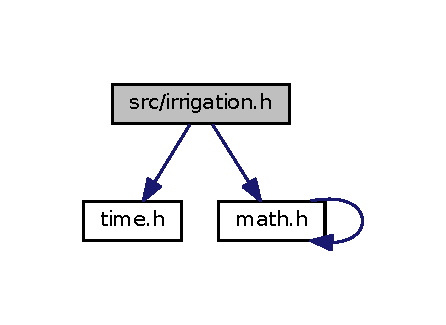
\includegraphics[width=214pt]{irrigation_8h__incl}
\end{center}
\end{figure}
This graph shows which files directly or indirectly include this file\+:
\nopagebreak
\begin{figure}[H]
\begin{center}
\leavevmode
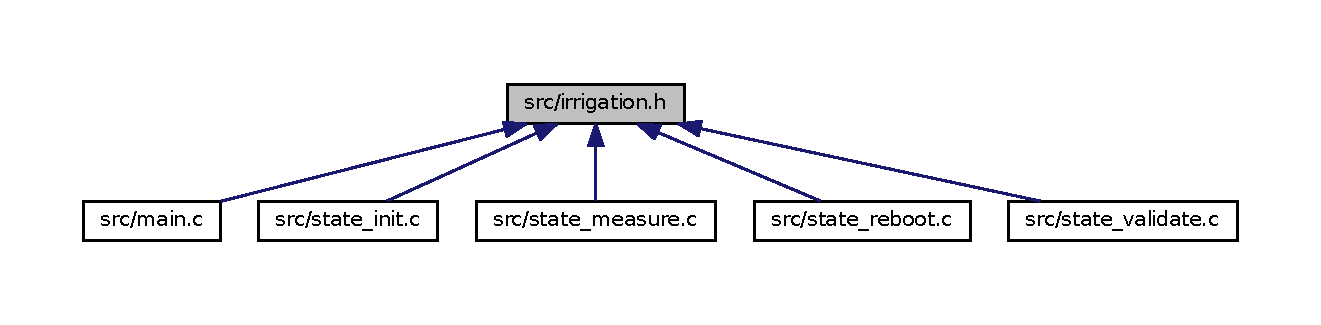
\includegraphics[width=350pt]{irrigation_8h__dep__incl}
\end{center}
\end{figure}
\subsection*{Classes}
\begin{DoxyCompactItemize}
\item 
struct \hyperlink{structirrigation__temperature__sample}{irrigation\+\_\+temperature\+\_\+sample}
\begin{DoxyCompactList}\small\item\em This is a timestamped temperature sample. \end{DoxyCompactList}\item 
struct \hyperlink{structirrigation__controller__status}{irrigation\+\_\+controller\+\_\+status}
\item 
struct \hyperlink{structirrigation__events}{irrigation\+\_\+events}
\begin{DoxyCompactList}\small\item\em The event callback functions for the irrigation controller core. \end{DoxyCompactList}\item 
struct \hyperlink{structirrigation__controller}{irrigation\+\_\+controller}
\begin{DoxyCompactList}\small\item\em Holds everything related to the irrigation controller. \end{DoxyCompactList}\end{DoxyCompactItemize}
\subsection*{Macros}
\begin{DoxyCompactItemize}
\item 
\#define \hyperlink{irrigation_8h_a98a17dc46f65ba67eb9c004ea48a9c2d}{time\+\_\+delta}(a,  b)~((float)(a.\+epoch -\/ b.\+epoch) + (float)(a.\+ms -\/ b.\+ms) / 1000.\+0)
\begin{DoxyCompactList}\small\item\em Calculates the time difference in seconds between two timestamps. \end{DoxyCompactList}\item 
\hypertarget{irrigation_8h_a8bb330be5fe982be9c1c28e70515043d}{}\#define {\bfseries \+\_\+\+I\+R\+R\+I\+G\+A\+T\+I\+O\+N\+\_\+\+H\+\_\+}\label{irrigation_8h_a8bb330be5fe982be9c1c28e70515043d}

\end{DoxyCompactItemize}
\subsection*{Enumerations}
\begin{DoxyCompactItemize}
\item 
enum \hyperlink{irrigation_8h_ac40bd72ec6942e213e454ebcacc92dc7}{irrigation\+\_\+status} \{ \\*
\hyperlink{irrigation_8h_ac40bd72ec6942e213e454ebcacc92dc7a64e8c241885100a4c6ee0dde8c084093}{irrigation\+\_\+status\+\_\+\+R\+E\+B\+O\+O\+T} = -\/2, 
\hyperlink{irrigation_8h_ac40bd72ec6942e213e454ebcacc92dc7a3d4b9190b0804578e02247c8cee11d8c}{irrigation\+\_\+status\+\_\+\+U\+N\+D\+E\+F\+I\+N\+E\+D} = -\/1, 
\hyperlink{irrigation_8h_ac40bd72ec6942e213e454ebcacc92dc7a0961e0972792be7ffcb4bf7aa64d4017}{irrigation\+\_\+status\+\_\+\+I\+N\+I\+T}, 
\hyperlink{irrigation_8h_ac40bd72ec6942e213e454ebcacc92dc7a0421b2d42223b25611688b6d2fe2d6e1}{irrigation\+\_\+status\+\_\+\+V\+A\+L\+I\+D\+A\+T\+E}, 
\\*
\hyperlink{irrigation_8h_ac40bd72ec6942e213e454ebcacc92dc7a1138583e9263588b98c16578bed06987}{irrigation\+\_\+status\+\_\+\+M\+E\+A\+S\+U\+R\+E}
 \}
\begin{DoxyCompactList}\small\item\em This is the state of the irrigation controller. \end{DoxyCompactList}\item 
enum \hyperlink{irrigation_8h_a9891f6b3b37611d2aebdb8601acdf6c6}{moisture\+\_\+sensor\+\_\+state} \{ \hyperlink{irrigation_8h_a9891f6b3b37611d2aebdb8601acdf6c6ad3f6b80b71bad74ea52dda2f31231cc3}{moisture\+\_\+sensor\+\_\+heating}, 
\hyperlink{irrigation_8h_a9891f6b3b37611d2aebdb8601acdf6c6a7e57547ef4980c1af315fd9937c976f0}{moisture\+\_\+sensor\+\_\+cooling}, 
\hyperlink{irrigation_8h_a9891f6b3b37611d2aebdb8601acdf6c6a4460d045ceb966a377b72d2825606fbd}{moisture\+\_\+sensor\+\_\+t1}, 
{\bfseries moisture\+\_\+sensor\+\_\+t2}
 \}
\begin{DoxyCompactList}\small\item\em This is the state of the moisture sensor. \end{DoxyCompactList}\end{DoxyCompactItemize}
\subsection*{Functions}
\begin{DoxyCompactItemize}
\item 
void \hyperlink{group__state__init_gaeca2f683660bf42f5258acd6aac353d0}{state\+\_\+init\+\_\+enter} (struct \hyperlink{structirrigation__controller}{irrigation\+\_\+controller} $\ast$controller)
\begin{DoxyCompactList}\small\item\em Reset all variables in the controller this state uses. \end{DoxyCompactList}\item 
void \hyperlink{group__state__init_ga5b5f5a7ec8534a643fb599efdee6ed4f}{state\+\_\+init\+\_\+run} (struct \hyperlink{structirrigation__controller}{irrigation\+\_\+controller} $\ast$controller)
\begin{DoxyCompactList}\small\item\em We will make a heart beat ramp for the status L\+E\+D while we wait for initial delay to complete. \end{DoxyCompactList}\item 
void \hyperlink{group__state__init_ga52863e306edb45d15c12acdecb7e5555}{state\+\_\+init\+\_\+exit} (struct \hyperlink{structirrigation__controller}{irrigation\+\_\+controller} $\ast$controller)
\begin{DoxyCompactList}\small\item\em Nothing has do be done before we leave this state. \end{DoxyCompactList}\item 
void \hyperlink{group__state__validate_gac0d41d4685bd461b3a613f6320405b79}{state\+\_\+validate\+\_\+enter} (struct \hyperlink{structirrigation__controller}{irrigation\+\_\+controller} $\ast$controller)
\begin{DoxyCompactList}\small\item\em We set up the validation timer and init the maximum and minim temperatured. \end{DoxyCompactList}\item 
void \hyperlink{group__state__validate_gaec38509b93f8a850919aa7a36e543ed5}{state\+\_\+validate\+\_\+run} (struct \hyperlink{structirrigation__controller}{irrigation\+\_\+controller} $\ast$controller)
\begin{DoxyCompactList}\small\item\em We have the heart beat L\+E\+D status and we update the minimum and maximum values while we continue to sample sensor data. \end{DoxyCompactList}\item 
void \hyperlink{group__state__validate_gac480e756742ffd9acd9bd21ac1e8885c}{state\+\_\+validate\+\_\+exit} (struct \hyperlink{structirrigation__controller}{irrigation\+\_\+controller} $\ast$controller)
\begin{DoxyCompactList}\small\item\em Nothing has to be done when we exit this state. \end{DoxyCompactList}\item 
\hypertarget{group__state__reboot_gab0e3409fa69ff96792cb5a768928a545}{}void {\bfseries state\+\_\+reboot\+\_\+enter} (struct \hyperlink{structirrigation__controller}{irrigation\+\_\+controller} $\ast$controller)\label{group__state__reboot_gab0e3409fa69ff96792cb5a768928a545}

\item 
\hypertarget{group__state__reboot_ga23cf1ecfb670c7c6c253a40705aa5caf}{}void {\bfseries state\+\_\+reboot\+\_\+run} (struct \hyperlink{structirrigation__controller}{irrigation\+\_\+controller} $\ast$controller)\label{group__state__reboot_ga23cf1ecfb670c7c6c253a40705aa5caf}

\item 
\hypertarget{group__state__reboot_gafbcdeb4b017f4350fb6ff51df410228b}{}void {\bfseries state\+\_\+reboot\+\_\+exit} (struct \hyperlink{structirrigation__controller}{irrigation\+\_\+controller} $\ast$controller)\label{group__state__reboot_gafbcdeb4b017f4350fb6ff51df410228b}

\item 
\hypertarget{group__state__measure_ga24a42892ba25be220bff68fc151e0be7}{}void {\bfseries state\+\_\+measure\+\_\+enter} (struct \hyperlink{structirrigation__controller}{irrigation\+\_\+controller} $\ast$controller)\label{group__state__measure_ga24a42892ba25be220bff68fc151e0be7}

\item 
\hypertarget{group__state__measure_ga410776694bde81bde92a0b6b178ac015}{}void {\bfseries state\+\_\+measure\+\_\+run} (struct \hyperlink{structirrigation__controller}{irrigation\+\_\+controller} $\ast$controller)\label{group__state__measure_ga410776694bde81bde92a0b6b178ac015}

\item 
\hypertarget{group__state__measure_ga0f85f8645f5311e776e85a3697517266}{}void {\bfseries state\+\_\+measure\+\_\+exit} (struct \hyperlink{structirrigation__controller}{irrigation\+\_\+controller} $\ast$controller)\label{group__state__measure_ga0f85f8645f5311e776e85a3697517266}

\item 
\hypertarget{irrigation_8h_a6440cc6e50bc4445698e203198648185}{}void {\bfseries status\+\_\+color} (int r, int g, int b)\label{irrigation_8h_a6440cc6e50bc4445698e203198648185}

\end{DoxyCompactItemize}


\subsection{Detailed Description}
Irrigation main include file. 



\subsection{Macro Definition Documentation}
\hypertarget{irrigation_8h_a98a17dc46f65ba67eb9c004ea48a9c2d}{}\index{irrigation.\+h@{irrigation.\+h}!time\+\_\+delta@{time\+\_\+delta}}
\index{time\+\_\+delta@{time\+\_\+delta}!irrigation.\+h@{irrigation.\+h}}
\subsubsection[{time\+\_\+delta}]{\setlength{\rightskip}{0pt plus 5cm}\#define time\+\_\+delta(
\begin{DoxyParamCaption}
\item[{}]{a, }
\item[{}]{b}
\end{DoxyParamCaption}
)~((float)(a.\+epoch -\/ b.\+epoch) + (float)(a.\+ms -\/ b.\+ms) / 1000.\+0)}\label{irrigation_8h_a98a17dc46f65ba67eb9c004ea48a9c2d}


Calculates the time difference in seconds between two timestamps. 


\begin{DoxyParams}{Parameters}
{\em a} & Time event A \\
\hline
{\em b} & Time event B\\
\hline
\end{DoxyParams}
\begin{DoxyReturn}{Returns}
Returns a -\/ b 
\end{DoxyReturn}


\subsection{Enumeration Type Documentation}
\hypertarget{irrigation_8h_ac40bd72ec6942e213e454ebcacc92dc7}{}\index{irrigation.\+h@{irrigation.\+h}!irrigation\+\_\+status@{irrigation\+\_\+status}}
\index{irrigation\+\_\+status@{irrigation\+\_\+status}!irrigation.\+h@{irrigation.\+h}}
\subsubsection[{irrigation\+\_\+status}]{\setlength{\rightskip}{0pt plus 5cm}enum {\bf irrigation\+\_\+status}}\label{irrigation_8h_ac40bd72ec6942e213e454ebcacc92dc7}


This is the state of the irrigation controller. 

\begin{Desc}
\item[Enumerator]\par
\begin{description}
\index{irrigation\+\_\+status\+\_\+\+R\+E\+B\+O\+O\+T@{irrigation\+\_\+status\+\_\+\+R\+E\+B\+O\+O\+T}!irrigation.\+h@{irrigation.\+h}}\index{irrigation.\+h@{irrigation.\+h}!irrigation\+\_\+status\+\_\+\+R\+E\+B\+O\+O\+T@{irrigation\+\_\+status\+\_\+\+R\+E\+B\+O\+O\+T}}\item[{\em 
\hypertarget{irrigation_8h_ac40bd72ec6942e213e454ebcacc92dc7a64e8c241885100a4c6ee0dde8c084093}{}irrigation\+\_\+status\+\_\+\+R\+E\+B\+O\+O\+T\label{irrigation_8h_ac40bd72ec6942e213e454ebcacc92dc7a64e8c241885100a4c6ee0dde8c084093}
}]If something goes terribly wrong we can set this to pending state and force a reboot. \index{irrigation\+\_\+status\+\_\+\+U\+N\+D\+E\+F\+I\+N\+E\+D@{irrigation\+\_\+status\+\_\+\+U\+N\+D\+E\+F\+I\+N\+E\+D}!irrigation.\+h@{irrigation.\+h}}\index{irrigation.\+h@{irrigation.\+h}!irrigation\+\_\+status\+\_\+\+U\+N\+D\+E\+F\+I\+N\+E\+D@{irrigation\+\_\+status\+\_\+\+U\+N\+D\+E\+F\+I\+N\+E\+D}}\item[{\em 
\hypertarget{irrigation_8h_ac40bd72ec6942e213e454ebcacc92dc7a3d4b9190b0804578e02247c8cee11d8c}{}irrigation\+\_\+status\+\_\+\+U\+N\+D\+E\+F\+I\+N\+E\+D\label{irrigation_8h_ac40bd72ec6942e213e454ebcacc92dc7a3d4b9190b0804578e02247c8cee11d8c}
}]This is the default sate but it is also used for the pending state when no pending state is set. \index{irrigation\+\_\+status\+\_\+\+I\+N\+I\+T@{irrigation\+\_\+status\+\_\+\+I\+N\+I\+T}!irrigation.\+h@{irrigation.\+h}}\index{irrigation.\+h@{irrigation.\+h}!irrigation\+\_\+status\+\_\+\+I\+N\+I\+T@{irrigation\+\_\+status\+\_\+\+I\+N\+I\+T}}\item[{\em 
\hypertarget{irrigation_8h_ac40bd72ec6942e213e454ebcacc92dc7a0961e0972792be7ffcb4bf7aa64d4017}{}irrigation\+\_\+status\+\_\+\+I\+N\+I\+T\label{irrigation_8h_ac40bd72ec6942e213e454ebcacc92dc7a0961e0972792be7ffcb4bf7aa64d4017}
}]Initialize the system. \index{irrigation\+\_\+status\+\_\+\+V\+A\+L\+I\+D\+A\+T\+E@{irrigation\+\_\+status\+\_\+\+V\+A\+L\+I\+D\+A\+T\+E}!irrigation.\+h@{irrigation.\+h}}\index{irrigation.\+h@{irrigation.\+h}!irrigation\+\_\+status\+\_\+\+V\+A\+L\+I\+D\+A\+T\+E@{irrigation\+\_\+status\+\_\+\+V\+A\+L\+I\+D\+A\+T\+E}}\item[{\em 
\hypertarget{irrigation_8h_ac40bd72ec6942e213e454ebcacc92dc7a0421b2d42223b25611688b6d2fe2d6e1}{}irrigation\+\_\+status\+\_\+\+V\+A\+L\+I\+D\+A\+T\+E\label{irrigation_8h_ac40bd72ec6942e213e454ebcacc92dc7a0421b2d42223b25611688b6d2fe2d6e1}
}]Validate the sensors. \index{irrigation\+\_\+status\+\_\+\+M\+E\+A\+S\+U\+R\+E@{irrigation\+\_\+status\+\_\+\+M\+E\+A\+S\+U\+R\+E}!irrigation.\+h@{irrigation.\+h}}\index{irrigation.\+h@{irrigation.\+h}!irrigation\+\_\+status\+\_\+\+M\+E\+A\+S\+U\+R\+E@{irrigation\+\_\+status\+\_\+\+M\+E\+A\+S\+U\+R\+E}}\item[{\em 
\hypertarget{irrigation_8h_ac40bd72ec6942e213e454ebcacc92dc7a1138583e9263588b98c16578bed06987}{}irrigation\+\_\+status\+\_\+\+M\+E\+A\+S\+U\+R\+E\label{irrigation_8h_ac40bd72ec6942e213e454ebcacc92dc7a1138583e9263588b98c16578bed06987}
}]Measure soil water content. \end{description}
\end{Desc}
\hypertarget{irrigation_8h_a9891f6b3b37611d2aebdb8601acdf6c6}{}\index{irrigation.\+h@{irrigation.\+h}!moisture\+\_\+sensor\+\_\+state@{moisture\+\_\+sensor\+\_\+state}}
\index{moisture\+\_\+sensor\+\_\+state@{moisture\+\_\+sensor\+\_\+state}!irrigation.\+h@{irrigation.\+h}}
\subsubsection[{moisture\+\_\+sensor\+\_\+state}]{\setlength{\rightskip}{0pt plus 5cm}enum {\bf moisture\+\_\+sensor\+\_\+state}}\label{irrigation_8h_a9891f6b3b37611d2aebdb8601acdf6c6}


This is the state of the moisture sensor. 

\begin{Desc}
\item[Enumerator]\par
\begin{description}
\index{moisture\+\_\+sensor\+\_\+heating@{moisture\+\_\+sensor\+\_\+heating}!irrigation.\+h@{irrigation.\+h}}\index{irrigation.\+h@{irrigation.\+h}!moisture\+\_\+sensor\+\_\+heating@{moisture\+\_\+sensor\+\_\+heating}}\item[{\em 
\hypertarget{irrigation_8h_a9891f6b3b37611d2aebdb8601acdf6c6ad3f6b80b71bad74ea52dda2f31231cc3}{}moisture\+\_\+sensor\+\_\+heating\label{irrigation_8h_a9891f6b3b37611d2aebdb8601acdf6c6ad3f6b80b71bad74ea52dda2f31231cc3}
}]The sensor is heating up. \index{moisture\+\_\+sensor\+\_\+cooling@{moisture\+\_\+sensor\+\_\+cooling}!irrigation.\+h@{irrigation.\+h}}\index{irrigation.\+h@{irrigation.\+h}!moisture\+\_\+sensor\+\_\+cooling@{moisture\+\_\+sensor\+\_\+cooling}}\item[{\em 
\hypertarget{irrigation_8h_a9891f6b3b37611d2aebdb8601acdf6c6a7e57547ef4980c1af315fd9937c976f0}{}moisture\+\_\+sensor\+\_\+cooling\label{irrigation_8h_a9891f6b3b37611d2aebdb8601acdf6c6a7e57547ef4980c1af315fd9937c976f0}
}]The sensor is cooling down. \index{moisture\+\_\+sensor\+\_\+t1@{moisture\+\_\+sensor\+\_\+t1}!irrigation.\+h@{irrigation.\+h}}\index{irrigation.\+h@{irrigation.\+h}!moisture\+\_\+sensor\+\_\+t1@{moisture\+\_\+sensor\+\_\+t1}}\item[{\em 
\hypertarget{irrigation_8h_a9891f6b3b37611d2aebdb8601acdf6c6a4460d045ceb966a377b72d2825606fbd}{}moisture\+\_\+sensor\+\_\+t1\label{irrigation_8h_a9891f6b3b37611d2aebdb8601acdf6c6a4460d045ceb966a377b72d2825606fbd}
}]\begin{DoxyRefDesc}{Todo}
\item[\hyperlink{todo__todo000003}{Todo}]t1 and t2 are not used for the moment \end{DoxyRefDesc}
\end{description}
\end{Desc}

\hypertarget{main_8c}{}\section{src/main.c File Reference}
\label{main_8c}\index{src/main.\+c@{src/main.\+c}}


Irrigation controller main file.  


{\ttfamily \#include \char`\"{}math.\+h\char`\"{}}\\*
{\ttfamily \#include \char`\"{}ws2812\+\_\+macro.\+h\char`\"{}}\\*
{\ttfamily \#include \char`\"{}usart\+\_\+macro.\+h\char`\"{}}\\*
{\ttfamily \#include \char`\"{}led\+\_\+macro.\+h\char`\"{}}\\*
{\ttfamily \#include \char`\"{}timer\+\_\+macro.\+h\char`\"{}}\\*
{\ttfamily \#include \char`\"{}systick.\+h\char`\"{}}\\*
{\ttfamily \#include \char`\"{}adc.\+h\char`\"{}}\\*
{\ttfamily \#include \char`\"{}time.\+h\char`\"{}}\\*
{\ttfamily \#include \char`\"{}filter.\+h\char`\"{}}\\*
{\ttfamily \#include \char`\"{}irrigation.\+h\char`\"{}}\\*
Include dependency graph for main.\+c\+:
\nopagebreak
\begin{figure}[H]
\begin{center}
\leavevmode
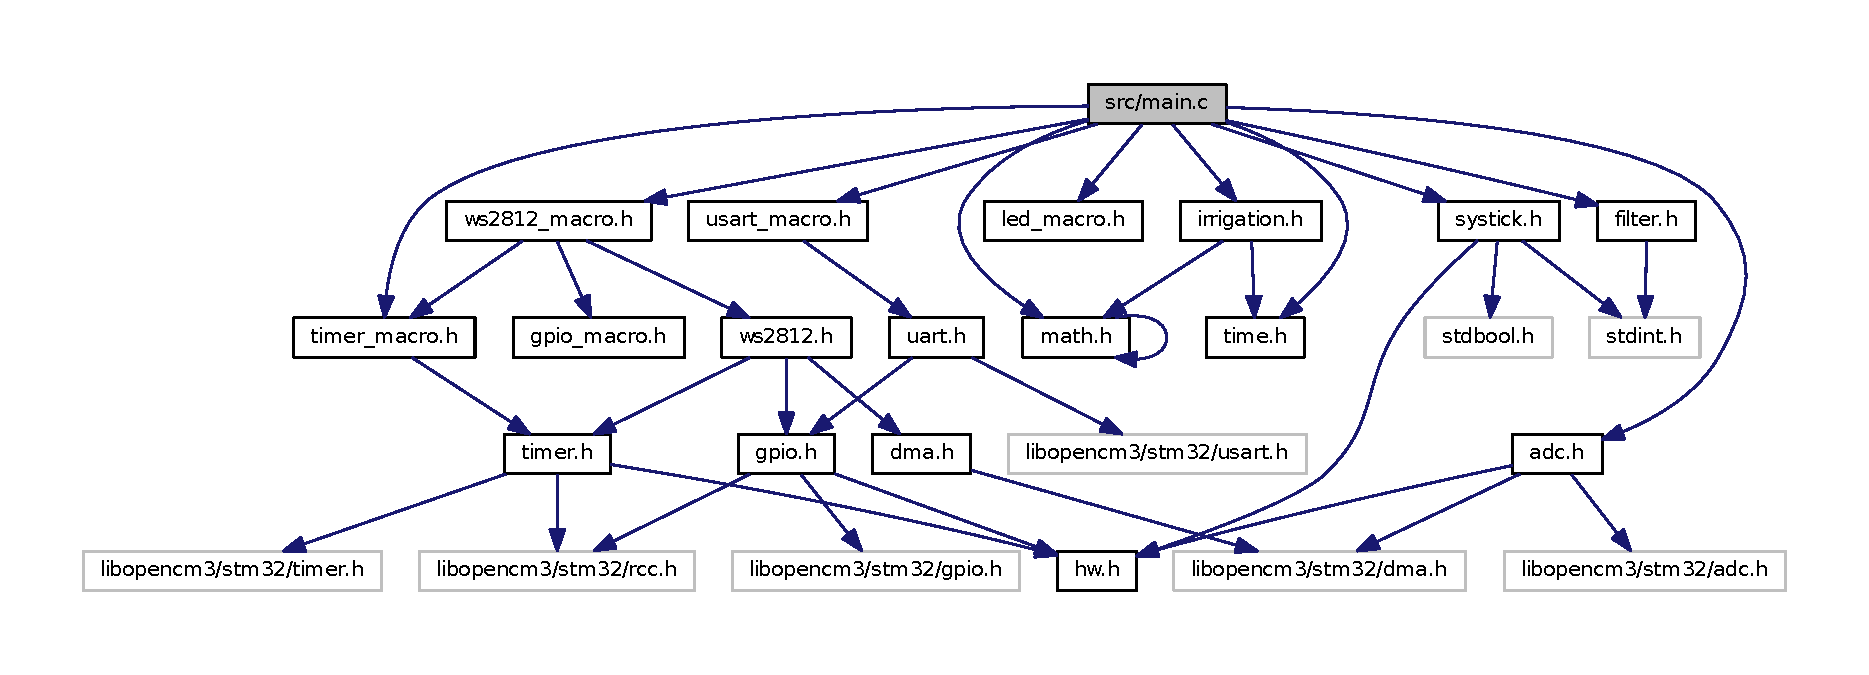
\includegraphics[width=350pt]{main_8c__incl}
\end{center}
\end{figure}
\subsection*{Classes}
\begin{DoxyCompactItemize}
\item 
struct \hyperlink{structstate}{state}
\end{DoxyCompactItemize}
\subsection*{Macros}
\begin{DoxyCompactItemize}
\item 
\hypertarget{main_8c_abedacb9f24c8951e3091cbbb69e35b9f}{}\#define {\bfseries N\+T\+C\+\_\+\+Filter\+\_\+\+Size}~250\label{main_8c_abedacb9f24c8951e3091cbbb69e35b9f}

\end{DoxyCompactItemize}
\subsection*{Functions}
\begin{DoxyCompactItemize}
\item 
\hypertarget{main_8c_aa423cbe2bea57704cca655826b2338c1}{}{\bfseries G\+P\+I\+O\+\_\+\+P\+O\+R\+T\+\_\+\+I\+N\+S\+T\+A\+N\+C\+E} (G\+P\+I\+O\+\_\+\+P\+A, G\+P\+I\+O\+A, R\+C\+C\+\_\+\+G\+P\+I\+O\+A)\label{main_8c_aa423cbe2bea57704cca655826b2338c1}

\item 
\hypertarget{main_8c_abebbe5a8f2ebcfc52329af1a2a452c32}{}{\bfseries G\+P\+I\+O\+\_\+\+P\+O\+R\+T\+\_\+\+I\+N\+S\+T\+A\+N\+C\+E} (G\+P\+I\+O\+\_\+\+P\+B, G\+P\+I\+O\+B, R\+C\+C\+\_\+\+G\+P\+I\+O\+B)\label{main_8c_abebbe5a8f2ebcfc52329af1a2a452c32}

\item 
\hypertarget{main_8c_ab051ec5725126430e405e5a598ccfe70}{}{\bfseries W\+S2812\+\_\+\+I\+N\+S\+T\+A\+N\+C\+E} (Status\+L\+E\+D, T\+I\+M\+E\+R1\+\_\+\+C\+C\+R3\+N\+\_\+\+D\+M\+A,\&G\+P\+I\+O\+\_\+\+P\+B, G\+P\+I\+O15, 1)\label{main_8c_ab051ec5725126430e405e5a598ccfe70}

\item 
\hypertarget{main_8c_a80f5b1b0fc5eac69c761e7388600dc59}{}{\bfseries U\+S\+A\+R\+T\+\_\+\+T\+X\+O\+N\+L\+Y\+\_\+\+I\+N\+S\+T\+A\+N\+C\+E} (Serial, U\+S\+A\+R\+T1, R\+C\+C\+\_\+\+U\+S\+A\+R\+T1, 921600, 0, 0, 0, 0,\&G\+P\+I\+O\+\_\+\+P\+A, G\+P\+I\+O\+\_\+\+U\+S\+A\+R\+T1\+\_\+\+T\+X)\label{main_8c_a80f5b1b0fc5eac69c761e7388600dc59}

\item 
\hypertarget{main_8c_a853c3748541a5efcdc0a0aef2a523eb9}{}{\bfseries T\+I\+M\+E\+R\+\_\+\+C\+C\+R\+\_\+\+I\+N\+S\+T\+A\+N\+C\+E} (Pump,\&G\+P\+I\+O\+\_\+\+P\+B, G\+P\+I\+O\+\_\+\+M\+O\+D\+E\+\_\+\+O\+U\+T\+P\+U\+T\+\_\+2\+\_\+\+M\+H\+Z, G\+P\+I\+O\+\_\+\+C\+N\+F\+\_\+\+O\+U\+T\+P\+U\+T\+\_\+\+A\+L\+T\+F\+N\+\_\+\+P\+U\+S\+H\+P\+U\+L\+L, G\+P\+I\+O0, T\+I\+M\+E\+R3\+\_\+\+C\+C\+R3, 4095, 0)\label{main_8c_a853c3748541a5efcdc0a0aef2a523eb9}

\item 
\hypertarget{main_8c_a9454d469f767dc72f29f51487317ba6d}{}{\bfseries T\+I\+M\+E\+R\+\_\+\+C\+C\+R\+\_\+\+I\+N\+S\+T\+A\+N\+C\+E} (Heater,\&G\+P\+I\+O\+\_\+\+P\+A, G\+P\+I\+O\+\_\+\+M\+O\+D\+E\+\_\+\+O\+U\+T\+P\+U\+T\+\_\+2\+\_\+\+M\+H\+Z, G\+P\+I\+O\+\_\+\+C\+N\+F\+\_\+\+O\+U\+T\+P\+U\+T\+\_\+\+A\+L\+T\+F\+N\+\_\+\+P\+U\+S\+H\+P\+U\+L\+L, G\+P\+I\+O2, T\+I\+M\+E\+R2\+\_\+\+C\+C\+R3, 4095, 0)\label{main_8c_a9454d469f767dc72f29f51487317ba6d}

\item 
\hypertarget{main_8c_a1f98adee46907f4bd29dc153ce25dcb7}{}{\bfseries G\+A\+M\+M\+A\+\_\+\+L\+U\+T\+\_\+8\+\_\+8\+\_\+\+E\+\_\+\+I\+N\+S\+T\+A\+N\+C\+E} (L\+E\+D\+\_\+\+Gamma)\label{main_8c_a1f98adee46907f4bd29dc153ce25dcb7}

\item 
\hypertarget{main_8c_a3ffc4d6ea2a7a8039f889967b7a7d7e3}{}{\bfseries G\+P\+I\+O\+\_\+\+P\+I\+N\+\_\+\+I\+N\+S\+T\+A\+N\+C\+E} (N\+T\+C\+\_\+pin,\&G\+P\+I\+O\+\_\+\+P\+A, G\+P\+I\+O\+\_\+\+M\+O\+D\+E\+\_\+\+I\+N\+P\+U\+T, G\+P\+I\+O\+\_\+\+C\+N\+F\+\_\+\+I\+N\+P\+U\+T\+\_\+\+A\+N\+A\+L\+O\+G, G\+P\+I\+O3)\label{main_8c_a3ffc4d6ea2a7a8039f889967b7a7d7e3}

\item 
void \hyperlink{main_8c_aabae29cd362c0001a2b417c9206cb330}{hw\+\_\+init\+\_\+state} (enum \hyperlink{hw_8h_a3c02952100e7d051b77cdf060ca0ba9b}{hw\+\_\+init\+\_\+state} \hyperlink{structstate}{state})
\begin{DoxyCompactList}\small\item\em This function prototype calls all perhipherals with the state as argument. \end{DoxyCompactList}\item 
\hypertarget{main_8c_afdd94f850b193691f1bfc60c724b542a}{}void {\bfseries sys\+\_\+tick\+\_\+handler} (void)\label{main_8c_afdd94f850b193691f1bfc60c724b542a}

\item 
\hypertarget{main_8c_a42ca7c9b89c22fcd9ec9aeed3e96b6c4}{}void {\bfseries get\+\_\+system\+\_\+time\+\_\+blocking} (struct \hyperlink{structsw__timer__system__time}{sw\+\_\+timer\+\_\+system\+\_\+time} $\ast$result)\label{main_8c_a42ca7c9b89c22fcd9ec9aeed3e96b6c4}

\item 
\hypertarget{main_8c_a8e3d66f43880efbd56cc2f68347b9b19}{}void {\bfseries dma1\+\_\+channel1\+\_\+isr} (void)\label{main_8c_a8e3d66f43880efbd56cc2f68347b9b19}

\item 
\hypertarget{main_8c_a6440cc6e50bc4445698e203198648185}{}void {\bfseries status\+\_\+color} (int r, int g, int b)\label{main_8c_a6440cc6e50bc4445698e203198648185}

\item 
\hypertarget{main_8c_ab8505b37986de5265d35fdaa3569b9af}{}void {\bfseries usart\+\_\+blocking\+\_\+tm} (struct \hyperlink{structusart}{usart} $\ast$\hyperlink{structusart}{usart}, struct \hyperlink{structsw__timer__system__time}{sw\+\_\+timer\+\_\+system\+\_\+time} $\ast$\hyperlink{structtm}{tm})\label{main_8c_ab8505b37986de5265d35fdaa3569b9af}

\item 
\hypertarget{main_8c_a85b9fa287bbc4012266648cbfe73ef47}{}struct \hyperlink{structstate}{state} $\ast$ {\bfseries get\+\_\+state} (enum \hyperlink{irrigation_8h_ac40bd72ec6942e213e454ebcacc92dc7}{irrigation\+\_\+status} status)\label{main_8c_a85b9fa287bbc4012266648cbfe73ef47}

\item 
\hypertarget{main_8c_a095a7fe46cf30b7abfbc4aac4b02c257}{}void {\bfseries report\+\_\+current\+\_\+temperature} (struct \hyperlink{structirrigation__controller}{irrigation\+\_\+controller} $\ast$controller)\label{main_8c_a095a7fe46cf30b7abfbc4aac4b02c257}

\item 
\hypertarget{main_8c_a2d729620635ca5fd1fe6d397b013ad06}{}void {\bfseries report\+\_\+validation\+\_\+temperatures} (struct \hyperlink{structirrigation__controller}{irrigation\+\_\+controller} $\ast$controller)\label{main_8c_a2d729620635ca5fd1fe6d397b013ad06}

\item 
\hypertarget{main_8c_a328fcba3c5cf7d17f02b4c5b76495653}{}void {\bfseries report\+\_\+sensor\+\_\+malfunction} (struct \hyperlink{structirrigation__controller}{irrigation\+\_\+controller} $\ast$controller)\label{main_8c_a328fcba3c5cf7d17f02b4c5b76495653}

\item 
\hypertarget{main_8c_afe20ef6128c561c493413063e7924081}{}void {\bfseries report\+\_\+sensor\+\_\+fluctuations} (struct \hyperlink{structirrigation__controller}{irrigation\+\_\+controller} $\ast$controller)\label{main_8c_afe20ef6128c561c493413063e7924081}

\item 
\hypertarget{main_8c_ae8259bbc867800edd5b8dc218f1a6693}{}void {\bfseries report\+\_\+msg\+\_\+note} (struct \hyperlink{structirrigation__controller}{irrigation\+\_\+controller} $\ast$controller, char $\ast$msg)\label{main_8c_ae8259bbc867800edd5b8dc218f1a6693}

\item 
\hypertarget{main_8c_a4ce529588e4fc671f721721ca40e9f2e}{}void {\bfseries report\+\_\+measurement\+\_\+data} (struct \hyperlink{structirrigation__controller}{irrigation\+\_\+controller} $\ast$controller, char $\ast$msg)\label{main_8c_a4ce529588e4fc671f721721ca40e9f2e}

\end{DoxyCompactItemize}
\subsection*{Variables}
\begin{DoxyCompactItemize}
\item 
struct \hyperlink{structsystick__config}{systick\+\_\+config} {\bfseries Systick\+\_\+config}
\item 
struct \hyperlink{structsystick}{systick} {\bfseries Systick}
\item 
struct \hyperlink{structadc__config}{adc\+\_\+config} {\bfseries N\+T\+C\+\_\+adc\+\_\+config}
\item 
\hypertarget{main_8c_a58930016c740c92d9007715fd9262f27}{}uint16\+\_\+t {\bfseries N\+T\+C\+\_\+buffer} \mbox{[}1\mbox{]}\label{main_8c_a58930016c740c92d9007715fd9262f27}

\item 
struct \hyperlink{structadc}{adc} {\bfseries N\+T\+C\+\_\+adc}
\item 
\hypertarget{main_8c_a5333e724c49577c06758ac990228568b}{}volatile uint32\+\_\+t {\bfseries N\+T\+C\+\_\+filter\+\_\+buffer} \mbox{[}N\+T\+C\+\_\+\+Filter\+\_\+\+Size\mbox{]}\label{main_8c_a5333e724c49577c06758ac990228568b}

\item 
struct \hyperlink{structfilter__rms}{filter\+\_\+rms} {\bfseries N\+T\+C\+\_\+filter}
\item 
\hypertarget{main_8c_ad6626ba12fbadd1981081605f892a7bb}{}volatile int {\bfseries sleep\+\_\+ms} = 0\label{main_8c_ad6626ba12fbadd1981081605f892a7bb}

\item 
\hypertarget{main_8c_a2d39b8e4f9506f28e2bdff70929287f6}{}volatile int {\bfseries N\+T\+C\+\_\+filtered\+\_\+value} = -\/1\label{main_8c_a2d39b8e4f9506f28e2bdff70929287f6}

\item 
\hypertarget{main_8c_a9d12c8106f421683f94175dd1c572624}{}volatile struct \hyperlink{structsw__timer__system__time}{sw\+\_\+timer\+\_\+system\+\_\+time} {\bfseries system\+\_\+time} = \{1420070400, 0\}\label{main_8c_a9d12c8106f421683f94175dd1c572624}

\item 
\hypertarget{main_8c_a153e3e14841d1967017a21ab4feacc19}{}volatile bool {\bfseries system\+\_\+time\+\_\+updated} =0\label{main_8c_a153e3e14841d1967017a21ab4feacc19}

\item 
\hypertarget{main_8c_a82cbd1bddefe1e9d0229cb36b068ec6d}{}const struct \hyperlink{structstate}{state} {\bfseries state\+\_\+init} = \{\hyperlink{group__state__init_gaeca2f683660bf42f5258acd6aac353d0}{state\+\_\+init\+\_\+enter}, \hyperlink{group__state__init_ga5b5f5a7ec8534a643fb599efdee6ed4f}{state\+\_\+init\+\_\+run}, \hyperlink{group__state__init_ga52863e306edb45d15c12acdecb7e5555}{state\+\_\+init\+\_\+exit}, \char`\"{}Init\char`\"{}\}\label{main_8c_a82cbd1bddefe1e9d0229cb36b068ec6d}

\item 
\hypertarget{main_8c_af5282fd583ec6d89886f7f7790721e29}{}const struct \hyperlink{structstate}{state} {\bfseries state\+\_\+validate} = \{\hyperlink{group__state__validate_gac0d41d4685bd461b3a613f6320405b79}{state\+\_\+validate\+\_\+enter}, \hyperlink{group__state__validate_gaec38509b93f8a850919aa7a36e543ed5}{state\+\_\+validate\+\_\+run}, \hyperlink{group__state__validate_gac480e756742ffd9acd9bd21ac1e8885c}{state\+\_\+validate\+\_\+exit}, \char`\"{}Validate temperature sensor\char`\"{}\}\label{main_8c_af5282fd583ec6d89886f7f7790721e29}

\item 
\hypertarget{main_8c_abc9312d41f1b93fd44e0cdad05313483}{}const struct \hyperlink{structstate}{state} {\bfseries state\+\_\+reboot} = \{state\+\_\+reboot\+\_\+enter, state\+\_\+reboot\+\_\+run, state\+\_\+reboot\+\_\+exit, \char`\"{}Reboot\char`\"{}\}\label{main_8c_abc9312d41f1b93fd44e0cdad05313483}

\item 
\hypertarget{main_8c_a3ce37ea920e9b7c6b383d70fe40233e7}{}const struct \hyperlink{structstate}{state} {\bfseries state\+\_\+measure} = \{state\+\_\+measure\+\_\+enter, state\+\_\+measure\+\_\+run, state\+\_\+measure\+\_\+exit, \char`\"{}Measure soil water content\char`\"{}\}\label{main_8c_a3ce37ea920e9b7c6b383d70fe40233e7}

\item 
struct \hyperlink{structirrigation__controller}{irrigation\+\_\+controller} {\bfseries ic}
\end{DoxyCompactItemize}


\subsection{Detailed Description}
Irrigation controller main file. 

\begin{DoxyRefDesc}{Todo}
\item[\hyperlink{todo__todo000005}{Todo}]systick, adc, moisture sensor, pwm output, filter\end{DoxyRefDesc}


\subsection{Function Documentation}
\hypertarget{main_8c_aabae29cd362c0001a2b417c9206cb330}{}\index{main.\+c@{main.\+c}!hw\+\_\+init\+\_\+state@{hw\+\_\+init\+\_\+state}}
\index{hw\+\_\+init\+\_\+state@{hw\+\_\+init\+\_\+state}!main.\+c@{main.\+c}}
\subsubsection[{hw\+\_\+init\+\_\+state}]{\setlength{\rightskip}{0pt plus 5cm}void {\bf hw\+\_\+init\+\_\+state} (
\begin{DoxyParamCaption}
\item[{enum {\bf hw\+\_\+init\+\_\+state}}]{state}
\end{DoxyParamCaption}
)}\label{main_8c_aabae29cd362c0001a2b417c9206cb330}


This function prototype calls all perhipherals with the state as argument. 



\subsection{Variable Documentation}
\hypertarget{main_8c_a2c433a8720f4e75971c7f216723aba26}{}\index{main.\+c@{main.\+c}!ic@{ic}}
\index{ic@{ic}!main.\+c@{main.\+c}}
\subsubsection[{ic}]{\setlength{\rightskip}{0pt plus 5cm}struct {\bf irrigation\+\_\+controller} ic}\label{main_8c_a2c433a8720f4e75971c7f216723aba26}
{\bfseries Initial value\+:}
\begin{DoxyCode}
= \{
    .events = \{
        .report\_validation\_temperatures = report\_validation\_temperatures,
        .report\_sensor\_malfunction = report\_sensor\_malfunction,
        .report\_sensor\_fluctuations = report\_sensor\_fluctuations,
        .report\_current\_temperature = report\_current\_temperature,
        .report\_msg\_note = report\_msg\_note,
        .report\_measurement\_data = report\_measurement\_data,
    \}
\}
\end{DoxyCode}
\hypertarget{main_8c_ab08aed4305f11ea61ea2ac93a524d34b}{}\index{main.\+c@{main.\+c}!N\+T\+C\+\_\+adc@{N\+T\+C\+\_\+adc}}
\index{N\+T\+C\+\_\+adc@{N\+T\+C\+\_\+adc}!main.\+c@{main.\+c}}
\subsubsection[{N\+T\+C\+\_\+adc}]{\setlength{\rightskip}{0pt plus 5cm}struct {\bf adc} N\+T\+C\+\_\+adc}\label{main_8c_ab08aed4305f11ea61ea2ac93a524d34b}
{\bfseries Initial value\+:}
\begin{DoxyCode}
= \{
    .configuration = &NTC\_adc\_config,
    .adc\_buffer = NTC\_buffer,
\}
\end{DoxyCode}
\hypertarget{main_8c_a9036c54a901bdc13978408f1babe6f78}{}\index{main.\+c@{main.\+c}!N\+T\+C\+\_\+adc\+\_\+config@{N\+T\+C\+\_\+adc\+\_\+config}}
\index{N\+T\+C\+\_\+adc\+\_\+config@{N\+T\+C\+\_\+adc\+\_\+config}!main.\+c@{main.\+c}}
\subsubsection[{N\+T\+C\+\_\+adc\+\_\+config}]{\setlength{\rightskip}{0pt plus 5cm}struct {\bf adc\+\_\+config} N\+T\+C\+\_\+adc\+\_\+config}\label{main_8c_a9036c54a901bdc13978408f1babe6f78}
{\bfseries Initial value\+:}
\begin{DoxyCode}
= \{
    .channel\_map = &(uint8\_t)\{3\},
    .channel\_count = 1,
\}
\end{DoxyCode}
\hypertarget{main_8c_ab0e81558ffe64a96a635a1a6af8ad8bd}{}\index{main.\+c@{main.\+c}!N\+T\+C\+\_\+filter@{N\+T\+C\+\_\+filter}}
\index{N\+T\+C\+\_\+filter@{N\+T\+C\+\_\+filter}!main.\+c@{main.\+c}}
\subsubsection[{N\+T\+C\+\_\+filter}]{\setlength{\rightskip}{0pt plus 5cm}struct {\bf filter\+\_\+rms} N\+T\+C\+\_\+filter}\label{main_8c_ab0e81558ffe64a96a635a1a6af8ad8bd}
{\bfseries Initial value\+:}
\begin{DoxyCode}
= \{
    .buffer = NTC\_filter\_buffer,
    .size = NTC\_Filter\_Size,
    .valid\_range = \{    
        .min = 1200,
        .max = 3400,
    \},
\}
\end{DoxyCode}
\hypertarget{main_8c_a8d0d8fb8a23aac2b6ac6d9e81e7b58e2}{}\index{main.\+c@{main.\+c}!Systick@{Systick}}
\index{Systick@{Systick}!main.\+c@{main.\+c}}
\subsubsection[{Systick}]{\setlength{\rightskip}{0pt plus 5cm}struct {\bf systick} Systick}\label{main_8c_a8d0d8fb8a23aac2b6ac6d9e81e7b58e2}
{\bfseries Initial value\+:}
\begin{DoxyCode}
= \{
    .configuration = &Systick\_config,
\}
\end{DoxyCode}
\hypertarget{main_8c_a4fb87b3684142c82865003df813ef052}{}\index{main.\+c@{main.\+c}!Systick\+\_\+config@{Systick\+\_\+config}}
\index{Systick\+\_\+config@{Systick\+\_\+config}!main.\+c@{main.\+c}}
\subsubsection[{Systick\+\_\+config}]{\setlength{\rightskip}{0pt plus 5cm}struct {\bf systick\+\_\+config} Systick\+\_\+config}\label{main_8c_a4fb87b3684142c82865003df813ef052}
{\bfseries Initial value\+:}
\begin{DoxyCode}
= \{
    .frequency = 1000,
    .auto\_start = 1,
\}
\end{DoxyCode}

\hypertarget{state__init_8c}{}\section{src/state\+\_\+init.c File Reference}
\label{state__init_8c}\index{src/state\+\_\+init.\+c@{src/state\+\_\+init.\+c}}


Initial state.  


{\ttfamily \#include \char`\"{}irrigation.\+h\char`\"{}}\\*
Include dependency graph for state\+\_\+init.\+c\+:\nopagebreak
\begin{figure}[H]
\begin{center}
\leavevmode
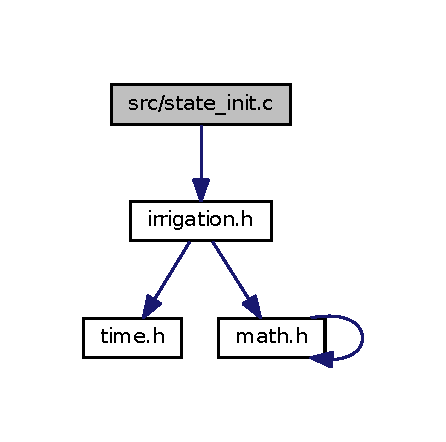
\includegraphics[width=214pt]{state__init_8c__incl}
\end{center}
\end{figure}
\subsection*{Functions}
\begin{DoxyCompactItemize}
\item 
void \hyperlink{group__state__init_gaeca2f683660bf42f5258acd6aac353d0}{state\+\_\+init\+\_\+enter} (struct \hyperlink{structirrigation__controller}{irrigation\+\_\+controller} $\ast$controller)
\begin{DoxyCompactList}\small\item\em Reset all variables in the controller this state uses. \end{DoxyCompactList}\item 
void \hyperlink{group__state__init_ga5b5f5a7ec8534a643fb599efdee6ed4f}{state\+\_\+init\+\_\+run} (struct \hyperlink{structirrigation__controller}{irrigation\+\_\+controller} $\ast$controller)
\begin{DoxyCompactList}\small\item\em We will make a heart beat ramp for the status L\+E\+D while we wait for initial delay to complete. \end{DoxyCompactList}\item 
void \hyperlink{group__state__init_ga52863e306edb45d15c12acdecb7e5555}{state\+\_\+init\+\_\+exit} (struct \hyperlink{structirrigation__controller}{irrigation\+\_\+controller} $\ast$controller)
\begin{DoxyCompactList}\small\item\em Nothing has do be done before we leave this state. \end{DoxyCompactList}\end{DoxyCompactItemize}


\subsection{Detailed Description}
Initial state. 


\hypertarget{state__measure_8c}{}\section{src/state\+\_\+measure.c File Reference}
\label{state__measure_8c}\index{src/state\+\_\+measure.\+c@{src/state\+\_\+measure.\+c}}


Measurement state.  


{\ttfamily \#include \char`\"{}irrigation.\+h\char`\"{}}\\*
Include dependency graph for state\+\_\+measure.\+c\+:\nopagebreak
\begin{figure}[H]
\begin{center}
\leavevmode
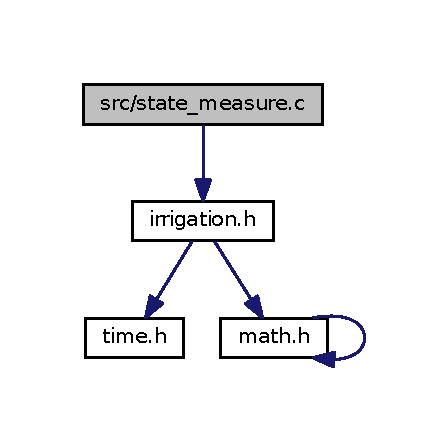
\includegraphics[width=215pt]{state__measure_8c__incl}
\end{center}
\end{figure}
\subsection*{Functions}
\begin{DoxyCompactItemize}
\item 
\hypertarget{group__state__measure_ga24a42892ba25be220bff68fc151e0be7}{}void {\bfseries state\+\_\+measure\+\_\+enter} (struct \hyperlink{structirrigation__controller}{irrigation\+\_\+controller} $\ast$controller)\label{group__state__measure_ga24a42892ba25be220bff68fc151e0be7}

\item 
\hypertarget{group__state__measure_ga410776694bde81bde92a0b6b178ac015}{}void {\bfseries state\+\_\+measure\+\_\+run} (struct \hyperlink{structirrigation__controller}{irrigation\+\_\+controller} $\ast$controller)\label{group__state__measure_ga410776694bde81bde92a0b6b178ac015}

\item 
\hypertarget{group__state__measure_ga0f85f8645f5311e776e85a3697517266}{}void {\bfseries state\+\_\+measure\+\_\+exit} (struct \hyperlink{structirrigation__controller}{irrigation\+\_\+controller} $\ast$controller)\label{group__state__measure_ga0f85f8645f5311e776e85a3697517266}

\end{DoxyCompactItemize}


\subsection{Detailed Description}
Measurement state. 


\hypertarget{state__reboot_8c}{}\section{src/state\+\_\+reboot.c File Reference}
\label{state__reboot_8c}\index{src/state\+\_\+reboot.\+c@{src/state\+\_\+reboot.\+c}}


Rebooting state.  


{\ttfamily \#include \char`\"{}irrigation.\+h\char`\"{}}\\*
Include dependency graph for state\+\_\+reboot.\+c\+:\nopagebreak
\begin{figure}[H]
\begin{center}
\leavevmode
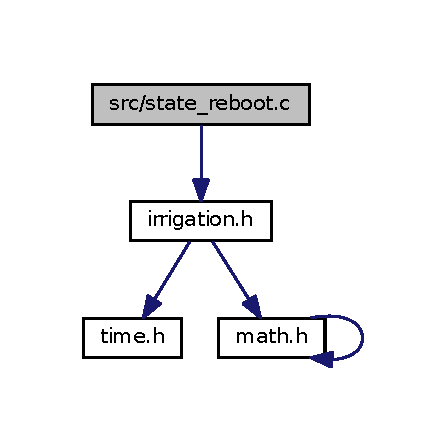
\includegraphics[width=214pt]{state__reboot_8c__incl}
\end{center}
\end{figure}
\subsection*{Functions}
\begin{DoxyCompactItemize}
\item 
\hypertarget{group__state__reboot_gab0e3409fa69ff96792cb5a768928a545}{}void {\bfseries state\+\_\+reboot\+\_\+enter} (struct \hyperlink{structirrigation__controller}{irrigation\+\_\+controller} $\ast$controller)\label{group__state__reboot_gab0e3409fa69ff96792cb5a768928a545}

\item 
\hypertarget{group__state__reboot_ga23cf1ecfb670c7c6c253a40705aa5caf}{}void {\bfseries state\+\_\+reboot\+\_\+run} (struct \hyperlink{structirrigation__controller}{irrigation\+\_\+controller} $\ast$controller)\label{group__state__reboot_ga23cf1ecfb670c7c6c253a40705aa5caf}

\item 
\hypertarget{group__state__reboot_gafbcdeb4b017f4350fb6ff51df410228b}{}void {\bfseries state\+\_\+reboot\+\_\+exit} (struct \hyperlink{structirrigation__controller}{irrigation\+\_\+controller} $\ast$controller)\label{group__state__reboot_gafbcdeb4b017f4350fb6ff51df410228b}

\end{DoxyCompactItemize}


\subsection{Detailed Description}
Rebooting state. 


\hypertarget{state__validate_8c}{}\section{src/state\+\_\+validate.c File Reference}
\label{state__validate_8c}\index{src/state\+\_\+validate.\+c@{src/state\+\_\+validate.\+c}}


Sensor validation state.  


{\ttfamily \#include \char`\"{}irrigation.\+h\char`\"{}}\\*
Include dependency graph for state\+\_\+validate.\+c\+:\nopagebreak
\begin{figure}[H]
\begin{center}
\leavevmode
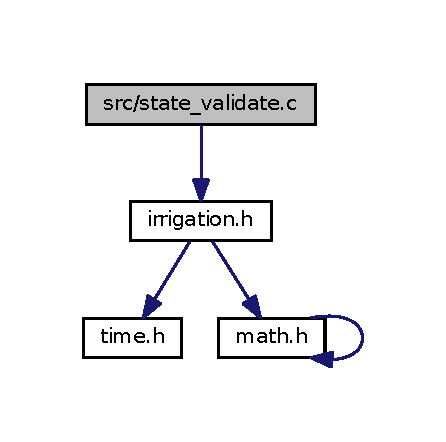
\includegraphics[width=214pt]{state__validate_8c__incl}
\end{center}
\end{figure}
\subsection*{Functions}
\begin{DoxyCompactItemize}
\item 
void \hyperlink{group__state__validate_gac0d41d4685bd461b3a613f6320405b79}{state\+\_\+validate\+\_\+enter} (struct \hyperlink{structirrigation__controller}{irrigation\+\_\+controller} $\ast$controller)
\begin{DoxyCompactList}\small\item\em We set up the validation timer and init the maximum and minim temperatured. \end{DoxyCompactList}\item 
void \hyperlink{group__state__validate_gaec38509b93f8a850919aa7a36e543ed5}{state\+\_\+validate\+\_\+run} (struct \hyperlink{structirrigation__controller}{irrigation\+\_\+controller} $\ast$controller)
\begin{DoxyCompactList}\small\item\em We have the heart beat L\+E\+D status and we update the minimum and maximum values while we continue to sample sensor data. \end{DoxyCompactList}\item 
void \hyperlink{group__state__validate_gac480e756742ffd9acd9bd21ac1e8885c}{state\+\_\+validate\+\_\+exit} (struct \hyperlink{structirrigation__controller}{irrigation\+\_\+controller} $\ast$controller)
\begin{DoxyCompactList}\small\item\em Nothing has to be done when we exit this state. \end{DoxyCompactList}\end{DoxyCompactItemize}


\subsection{Detailed Description}
Sensor validation state. 


%--- End generated contents ---

% Index
\backmatter
\newpage
\phantomsection
\clearemptydoublepage
\addcontentsline{toc}{chapter}{Index}
\printindex

\end{document}
